%-------------------------------------------------------------------------------
% Document
%-------------------------------------------------------------------------------
\documentclass[12pt,oneside,openany,a4paper,afrikaans,english]{memoir}
\OnehalfSpacing
%-------------------------------------------------------------------------------
% Packages
%-------------------------------------------------------------------------------
\usepackage[PhD,wideblock]{usthesis}
\usepackage{babel}
\usepackage[T1]{fontenc}
\usepackage{graphicx}
\usepackage{float} 
\usepackage{color}
\usepackage{eso-pic}
\usepackage[separate-uncertainty=true]{siunitx}
\usepackage{usbib}
\usepackage{subcaption}
\usepackage[labelfont=bf]{caption}
\usepackage[dvipsnames]{xcolor}
\usepackage{hyperref} 
\usepackage[nameinlink]{cleveref}
\usepackage[LGRgreek]{mathastext}

%-------------------------------------------------------------------------------
% Various settings
%-------------------------------------------------------------------------------
\bibliographystyle{usmeg-a}
\newcommand*{\WaterMark}[2][0.15\paperwidth]{%
    \AddToShipoutPicture*{\AtTextCenter{%
        \parbox[c]{0pt}{\makebox[0pt][c]{%
            \includegraphics[width=#1]{#2}}}}}}
\definecolor{lightblue}{RGB}{49,130,189}
\hypersetup{
	colorlinks=true,
	allcolors=lightblue,
	linktoc=page,
	}

%-------------------------------------------------------------------------------
% Special units
%-------------------------------------------------------------------------------
\DeclareSIUnit\Molar{\textsc{m}}


%-------------------------------------------------------------------------------
% Metadata
%-------------------------------------------------------------------------------
\title{\vspace*{1cm}INVESTIGATING THE ROLE OF RILMENIDINE AND SPERMIDINE ON AUTOPHAGIC FLUX AND CELL DEATH IN A MODEL OF ALZHEIMER'S DISEASE} 
\author{D.\ Lumkwana}{Dumisile Lumkwana}
\degree{PhD}{Doctor of Philosophy in Physiological Sciences}
\supervisor{Prof.\ B.\ Loos}
\cosupervisor{Prof.\ C.\ Kinnear}
\adress{Department of Physiological Sciences\\University of Stellenbosch\\Private Bag X1, Matieland 7602, South Africa.}
\faculty{Faculty of Sciences}
\ThesisDescript{ 
  \vspace*{2cm}
Dissertation presented for the degree of Doctor of Philosophy in Physiological Sciences, in the Faculty of Science at Stellenbosch University}
\setdate{12}{2019}
\SetSponsor{The financial assistance of the National Research Foundation (NRF) towards this research is hereby acknowledged. Opinions expressed and conclusions arrived at, are those of the author and are not necessarily to be attributed to the NRF.}
\begin{document}

%-------------------------------------------------------------------------------
% Front Matter
%-------------------------------------------------------------------------------
\frontmatter 
%-------------------------------------------------------------------------------
% Titlepage
%-------------------------------------------------------------------------------
\WaterMark[0.15\paperwidth]{UScrest-WM} 
\TitlePage

%-------------------------------------------------------------------------------
% Declaration page
%-------------------------------------------------------------------------------
\chapter{Declaration}
By submitting this dissertation electronically, I declare that the entirety of the work contained therein is my own, original work, that I am the sole author thereof (save to the extent explicitly otherwise stated), that reproduction and publication thereof by \mbox{Stellenbosch University} will not infringe any third party rights and that I have not \mbox{previously} in its entirety or in part submitted it for obtaining any qualification. \\ \\

\noindent
\begin{tabular}{@{}ll}
\textbf{Date:} & November 4, 2019 \\ 
\textbf{Name:} & Dumisile Lumkwana \\ 
\end{tabular}

\vspace*{\fill}
\begin{center}
Copyright $\textcopyright$ Stellenbosch University \\
All rights reserved.
\end{center}

%-------------------------------------------------------------------------------
% Abstract
%-------------------------------------------------------------------------------
\chapter{Abstract}
\newpage

\chapter{Opsomming}
\newpage

%-------------------------------------------------------------------------------
% Acknowledgements
%-------------------------------------------------------------------------------
\chapter{Acknowledgements}
\newpage

%-------------------------------------------------------------------------------
% Table and Lists of Content
%-------------------------------------------------------------------------------
\setcounter{secnumdepth}{4}
\setcounter{tocdepth}{4}

\tableofcontents
\newpage

\listoffigures
\newpage

\listoftables
\newpage

\chapter*{Nomenclature}
\addcontentsline{toc}{chapter}{Nomenclature}
\subsection*{Abbreviations}
\begin{itemize}[leftmargin=*,wide=0pt,]
\DTLforeach*{acronyms}{\thisAcronym=Acronym,\thisDesc=Description}
   {\item[] \textbf{\thisAcronym} \thisDesc}
\end{itemize}

\subsection*{Units of Measurements}
\begin{itemize}[leftmargin=*,wide=0pt,]
\DTLforeach*{units}{\thisUnit=Unit,\thisDesc=Description}
   {\item[] \textbf{\thisUnit} \thisDesc}
\end{itemize}


%-------------------------------------------------------------------------------
% Main Matter
%-------------------------------------------------------------------------------
\mainmatter
\chapter{Literature review}
\section{Introduction}
Alzheimer’s disease (AD) is the most common neurodegenerative disease and a leading cause of dementia in the elderly \citep{andrieu2015}. This disease is characterized by a progressive loss of synapses and neurons in certain brain regions (e.g. cerebral cortex and hippocampus), leading to impaired memory and deterioration of cognitive functions \citep{dekosky1990,scheff2006,zare-shahabadi2015}, thus necessitating full-time medical care \citep{prince2013}. Currently the disease is incurable. Although a lot of efforts have been directed towards developing AD disease modifying therapies, current treatment strategies are aimed at ameliorating disease symptoms alone \citep{anand2014,disanto2013}. Age is the most prominent risk factor for AD and about 44 million people are currently affected globally. While only 5 \% of individuals over the age of 65 years are affected by AD, the prevalence doubles with every 5 years of increasing age \citep{pimenova2018,qiu2009}. Given the rapidly aging population in first-and third- world countries, the prevalence of AD is predicted to rise to 81 million by 2025 \citep{AlzheimersAssociation2014,Ferri2005}. Moreover, it has been estimated that by 2050, 22 \% of the global population will be over the age of 60, with the majority residing in the developing nations \citep{Annear2015,Paddick2013}. In South Africa, there is limited statistics on the prevalence of AD. According to the census conducted in 2011, there are approximately 2.2 million people with some form of dementia. Very little is known about the prevalence of dementia and how it impacts on older adults residing in low and middle classes, as well as in the rural areas, where most of the adult population reside. Despite of this, it was reported that about 79 \% of patients were being cared for by family members \citep{Kalula2010}. In the continued absence of effective therapeutic strategies to either delay or slow down the disease progression, AD will pose a tremendously burden on the healthcare and social services. 

AD is a multifactorial disease that is highly complex, with genetic as well as environmental causes \citep{Dorszewska2016}. This disease is classified into two subsets. The first being the early-onset Familial Alzheimer’s disease (FAD, onset $<$ 65), which contributes to the least cases of AD (1-5 \%) with strong genetic association \citep{Musiek2015,Reitz2014,Swerdlow2007}. The second being sporadic late-onset Alzheimer’s disease (LOAD, onset $\geq$ 65) which contributes to the majority of all AD cases ($>$ 95 \%), \citep{Musiek2015,Reitz2014,Swerdlow2007}, with an unclear cause \citep{Dorszewska2016,pimenova2018}. Certain genes such as amyloid precursor protein (APP), Presenilin 1 (PSEN1) and Presenilin 2  (PSEN2) are responsible for occurrence of FAD, while APOE gene is responsible for LOAD \citep{Dorszewska2016}.

AD pathology occurs in 5 stages; the pre-symptomatic, Mild Cognitive Impairment (MCI), mild AD, moderate AD and severe AD \citep{Caldwell2015}. The first two stages encompasses a prodromal stage, which, in the majority of cases, precedes symptom onset by several years (at least 20 - 30 years) \citep{Caldwell2015,Caselli2013,Penn1993}. During this time, pathological molecular changes occur inside the brain and are present as two molecular hallmarks which occur as a result of perturbations in cellular proteostasis. The senile plaques, which are extracellular deposits of amyloid beta ($A\beta$)
peptides, and intraneuronal neurofibrillary tangles (NFTs), which are somatic inclusions of hyperphosphorylated, microtubule-associated protein tau, respectively \citep{Mattson2008} (\Cref{fig:10_AD_hallmarks}). To better understand the multifactorial pathophysiology of AD, several hypothesis have been put forward, including the amyloid cascade hypothesis (ACH), the cholinergic and tau hypothesis, as well as inflammation \citep{Kurz2011}; however, many molecular aspects and their dynamic changes during disease progression remain unclear. The ACH, the most widely accepted mechanistic hypothesis for AD, posits that an imbalance between the production and clearance of ($A\beta$) peptides is a very early, often initiating factor in disease onset \citep{Hardy2009,Hardy1992}.

\begin{figure}[!htbp]
  \includegraphics[width=\linewidth]{figures/chapter10/10_AD_hallmarks}
  \caption[Pathological hallmarks of AD]{. Pathological hallmarks of AD. Micrograph showing NFTs (arrows) and $A\beta$ plaques (arrowhead) in the AD brain \citep{Nixon2007} .}
  \label{fig:10_AD_hallmarks}
\end{figure}

Proteolytic systems; the ubiquitin-proteasome system (UPS) and the lysyosomal systems [the autophagy-lysosomal pathway (ALP) and the endocytic- lysosomal pathway (ELP)] are responsible for the degradation of mis-folded or aggregated proteins in order to maintain cellular homeostasis. For example, the UPS targets and degrades short-lived proteins in the cytoplasm and nucleus, while the lysosomal system removes primarily long lived cytoplasmic proteins and damaged organelles \citep{Ravikumar2003,Rubinsztein2005}. A large body of evidence implicates these proteolytic systems in the AD pathophysiology. Dysfunction of these system has been well documented in AD pathophysiology and although extracellular $A\beta$ plaques and intraneuronal NFTs are defining hallmarks of AD neuropathology, a growing body of literature suggests that deficits in the autophagy–lysosomal pathway are likely to precede the formation of these pathological hallmarks \citep{Cataldo2000,Nixon2011,Perez2015,zare-shahabadi2015}, suggesting a potential causality. More recently, a systems biology study highlighted the pivotal role of dysregulated autophagy in neurodegenerative diseases, where toxic protein aggregates and damaged organelles accumulate within specific types of neurons and lead to neuronal dysfunction and ultimately, demise \citep{Caberlotto2014}.

Although we have advanced our understanding of the molecular machinery that regulates the rate of protein degradation through autophagy at basal levels and the many aspects of its dysfunction in AD, the deviation of autophagic activity from basal levels and its change during disease pathogenesis in neuronal tissue remains largely unclear. Over the recent years, we have made substantial progress in modulating autophagy using pharmacological agents \citep{Berger2006,Hebron2013,Ravikumar2002,Ravikumar2004,Rose2010} or lifestyle interventions \citep{Alirezaei2010,Kuma2004,Mizushima2004a,Scott2004} \textit{in vitro} and \textit{in vivo}; yet many questions regarding an effective implementation of autophagy control remain unanswered. Therefore understanding the deviation of autophagic activity from basal levels and its change during disease pathogenesis as well as targeting or modulating autophagy activity precisely with the aim to restore autophagic flux may drive the development of better targeted therapeutic interventions that will slow down the disease progression and ultimately curing the disease instead of treating the symptoms. In this review, we start by describing neuronal metabolism and their metabolic profile and move to the involvement of reactive oxygen species in neurodegeneration, focusing on the role of oxidative stress and mitochondrial dysfunction in the pathogenesis of AD. We then turn our focus to amyloid beta biogenesis and its pathology in AD.  We highlight the recent advances in the use super resolution techniques in molecular biology. We introduce autophagy and its molecular machinery and discuss its efficiency and essential function in neuronal cells, followed by its role in neurodegenerative diseases. We discuss how autophagic flux may differ in brain regions, and how the deviation of flux may relate to the state of protein aggregation in pathology. Furthermore, we review studies that localize the defect in autophagy in AD and assess the relationship between autophagic flux and neuronal cell death. Finally, we indicate the importance of accurately measuring and targeting autophagy and provide an overview of how autophagy may be modulated for therapeutic purposes in various model systems aimed at restoring autophagic flux. 

\section{Neuronal metabolism}
A brain is made up of two cells types, neurons and astrocytes, which are highly interconnected and form functional networks through their spatial organization. The co-dependency of these cells types is reflected by their metabolic profiles where different yet complimentary pathways are used \citep{Belanger2011,Schonfeld2013}. The brain has a high energy demand. This is evident by the fact that 20 \% of oxygen and 25 \% of the glucose utilized by the human body is dedicated to only cerebral function, yet the brain encompasses only 2 \% of the total body mass \citep{Belanger2011}. This means, uninterrupted supply of energy substrates from the circulation is required to meet the energy demands. Glucose is the main substrate of energy in the brain 
\citep{Dienel2012,Pellerin2012}, however, other energy substrates such as lactate, pyruvate, glutamate, and glutamine can be utilized \citep{Zielke2009}.

Glucose is delivered into a cell via specific glucose transporters (GLUTs) and once inside, it is phosphorylated by an enzyme called hexokinase (HK) to generate glucose-6-phosphate (glucose-6P) \citep{Belanger2011,Herrero-Mendez2009}. The latter can enter three main metabolic pathways; glycolysis, pentose phosphate pathway (PPP), and glycogenesis in order to produce adenosine triphosphate (ATP). In glycolysis, glucose-6P is metabolized to produce pyruvate, 2 ATP molecules and NADH (nicotinamide adenine dinucleotide) \citep{Belanger2011}. Pyruvate can be metabolised further in the tricarboxylic acid (TCA) cycle and oxidative phosphorylation (OxPhos) in the mitochondria using oxygen to generate 30 - 34 ATP molecules and CO\textsubscript{2} or it can be reduced to lactate by lactate dehydrogenase (LDH) in the cytosol \citep{Belanger2011}. In PPP, glucose-6P is metabolized to generate NADPH (nicotinamide adenine dinucleotide phosphate), while in glycogenesis, it is stored as glycogen, with the latter occurring in astrocytes \citep{Belanger2011} (\Cref{fig:10_glucose_metabolism}). More importantly, astrocytes and neurons have the ability to oxidize glucose and/or lactate \citep{Zielke2009}.

\begin{figure}[!htbp]
  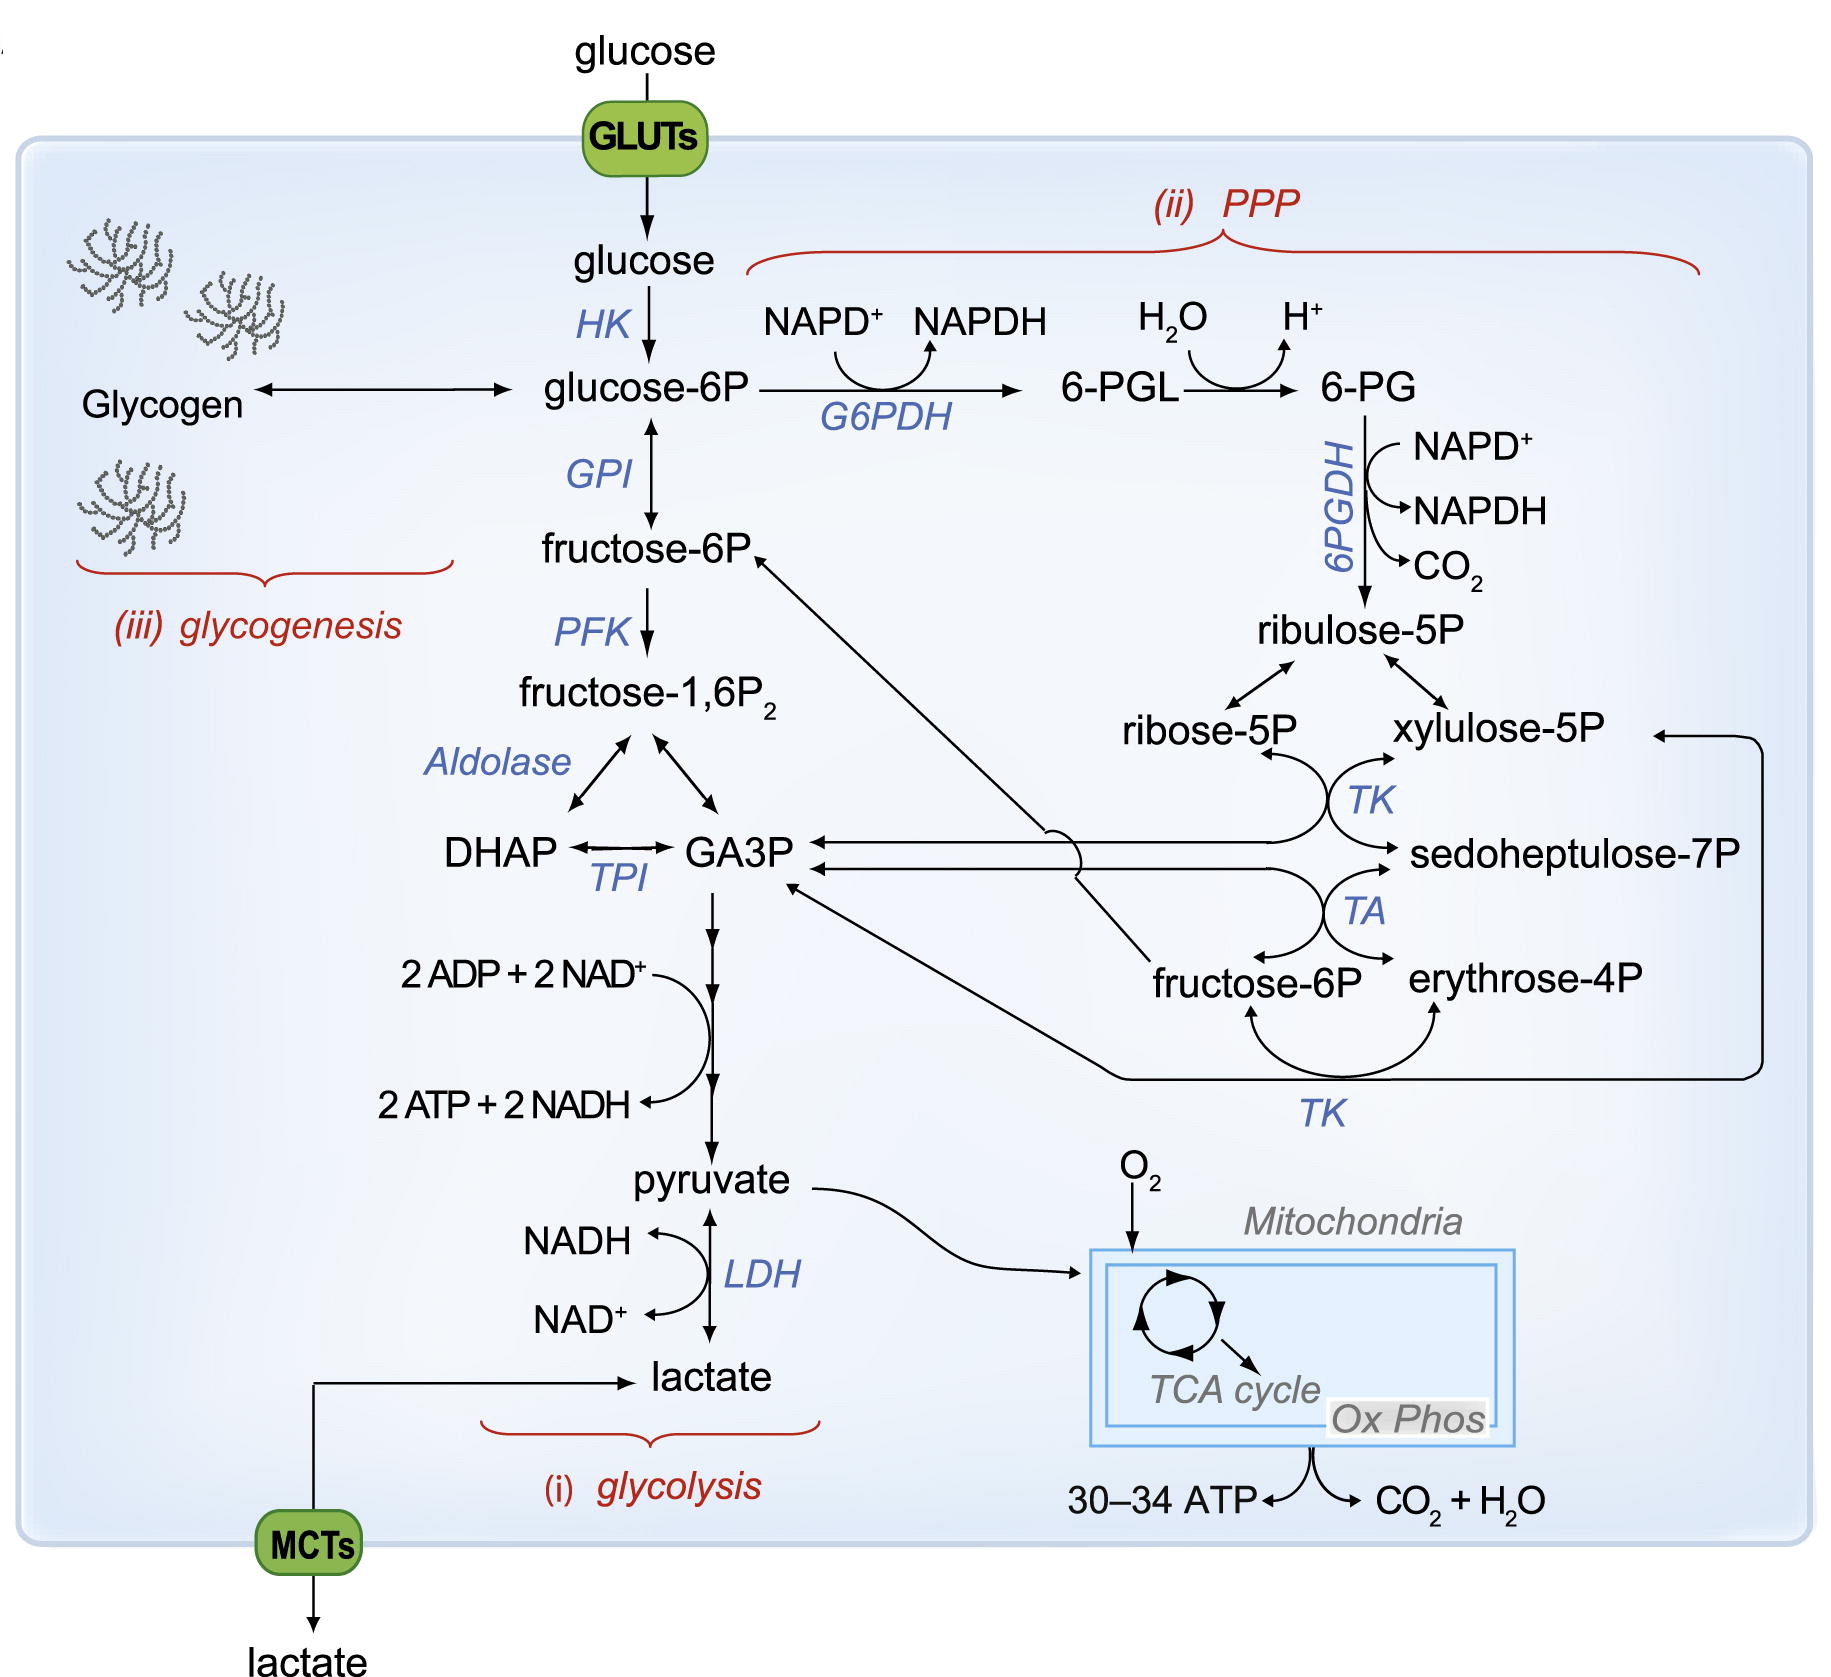
\includegraphics[width=\linewidth]{figures/chapter10/10_glucose_metabolism}
  \caption[Glucose metabolism]{Glucose metabolism. A schematic diagram showing three main pathways for glucose metabolism; glycolysis, pentose phosphate pathway, and glycogenesis \citep{Belanger2011} .}
  \label{fig:10_glucose_metabolism}
\end{figure}

\subsection{Metabolic profile of neurons}
Neurons are post-mitotic, highly differentiated cells that are characterized by high energy demands. This is due to their high levels of protein synthesis, which consumes high amount of ATP within the mammalian cells \citep{Buttgereit1995}. Neurons depend almost exclusively on the energy produced through OxPhos (30 - 34 ATP molecules) compared to glycolysis (2 ATP) in order to meet their high energy demand needed to perform cellular functions, such as synaptic plasticity and neurotransmitter synthesis \citep{Cenini2019,Mattson2008,Schonfeld2013}. Mounting evidence demonstrate that neurons are capable of using lactate as an energy substrate \citep{Boumezbeur2010,Bouzier2000,Serres2005} and prefer lactate over glucose when both substrates are available \citep{Bouzier-Sore2006,Itoh2003}. Thus the specific characteristics of neurons are probably underly their distinct metabolic profile. For example, glycolytic enzyme 6-phosphofructose-2-kinase/fructose-2, 6-bisphosphatase-3 (PFKFB3) is highly expressed in astrocytes, but virtually absent in neurons because of a constant proteasomal degradation \citep{Almeida2004,Herrero-Mendez2009}. Because of this, neurons unlike astrocytes display a lower glycolytic rate, and thus cannot upregulate this pathway in response to cellular stress \citep{Almeida2004,Herrero-Mendez2009}. Indeed, a previous study showed that upregulation of glycolysis via PFKFB3 in neurons is in fact detrimental, resulting to oxidative stress and apoptosis \citep{Herrero-Mendez2009}. In this study, it was though that the upregulation of glycolysis occurs at a cost of PPP metabolism that is needed to produce NADPH, an antioxidant vital for maintaining cellular redox state \citep{Herrero-Mendez2009}. Evidently, it has been shown that neurons have low NADPH compared to astrocytes \citep{Ben-Yoseph1996,Garcia-Nogales2003}, and since antioxidant system and the related enzymes are important for maintaining neuronal integrity and survival by keeping the levels of reactive oxygen species (ROS) relatively low \citep{Cenini2019}, it is not surprising that neurons are vulnerable to oxidative damage, implicated in neurodegeneration.

\section{ROS and its role in neurodegeneration}
ROS are a group of reactive molecules that are produced naturally in biological systems as part of normal cellular metabolism and are important in maintaining cellular homeostasis \citep{Cenini2019}. These include superoxide (O\textsubscript{2}\textsuperscript{-}), hydroxyl radical ($\cdot$OH), hydroxyl ion (OH\textsuperscript{-}) and hydrogen peroxide (H\textsubscript{2}O\textsubscript{2}), all of which are generated from oxygen. O\textsubscript{2}\textsuperscript{-} is generated from oxygen in the mitochondria as a result of the respiratory chain complex or NADPH oxidase and can be converted by superoxide dismutase (SOD) enzyme to produce H\textsubscript{2}0\textsubscript{2}. The later  in turn can be converted to other types of ROS, for example $\cdot$OH and OH\textsuperscript{-} \citep{Kim2015a}, with $\cdot$OH being the most reactive ROS responsible for cytotoxicity \citep{Bolisetty2013}.

Under physiological conditions, ROS levels are maintained at relatively low by antioxidant system \citep{Dasuri2013,Gandhi2012}, and are involved cellular processes such as inflammation, immune response, cell survival, synaptic plasticity, learning, and memory \citep{Cenini2019,Kishida2007,Liu2017}. However, increased ROS production can be harmful because of its ability to oxidise nucleic acids, protein and lipids \citep{Wang2014}. In fact, increased ROS accumulation has been implicated in oxidative stress, mitochondrial dysfunction and in gliosis. However, role of ROS in gliosis is poorly understood and only one study provides evidence \citep{Kishida2007}.

Excessive accumulation of ROS due failure of antioxidant system or increased ROS production can result in oxidative stress, defined as an imbalance between rate of ROS production and clearance \citep{Wang2014}. High levels of oxidative stress have been implicated in aging and in the pathogenesis of various neurodegenerative diseases \citep{Bonda2010,Cenini2019,Liu2017,Shibata2008}. Neurons are mostly susceptible to oxidative stress and damage due to its high oxygen consumption, high energy demand, low antioxidant defenses as well as high abundance of polyunsaturated fatty acid which are susceptible to lipid peroxidation \citep{Cobley2018}. Thus, it is not surprising that ROS induced oxidative damage is widely reported in AD. In addition, since mitochondria are the major source of ROS production and the main target of oxidative stress, progressive mitochondrial dysfunction has also been implicated in the pathogenesis of AD \citep{Swerdlow2007}. The involvement of oxidative stress and mitochondrial damage in AD has been demonstrated in different models and are described below. 

\subsection{Evidence of oxidative stress in AD}
Oxidative damage is one of the earliest events in AD \citep{Nunomura2001}. This is supported by several studies that demonstrated elevated levels of oxidative stress in patients with mild cognitive impairment (MCI) \citep{Ansari2010,Pratico2004,Williams2006}. In addition, antioxidants including uric acid, vitamin C and E as well as antioxidant enzyme SOD were found to be decreased in MCI patients \citep{Rinaldi2003,Torres2011}. Increased oxidative stress has also been implicated in AD. Excessive production of ROS is thought to play an essential role in the accumulation and deposition of $A\beta$ peptides \citep{Bonda2010}. \citet{Ferreiro2008} reported that $A\beta$ plaques depleted Ca\textsuperscript{2+}  (calcium) ion storage in the endoplasmic reticulum (ER), leading to in cytosolic Ca\textsuperscript{2+} overload, which resulted in the reduction of endogenous GSH (glutathione) levels and ROS accumulation. In addition, increased H\textsubscript{2}O\textsubscript{2} levels and increased peroxidation of proteins and lipids were shown in transgenic mouse expressing APP/PS-1, suggesting that $A\beta$ may exacerbate oxidative stress in AD \citep{Matsuoka2001,Zhao2013}. In addition, products of lipid peroxidation such as 4-hydroxynonal (4HNE), malondialdehyde (MDA), and 2 propenal (acrolein) have been found to be elevated in multiple studies performed in patient with AD \citep{Wang2014,Zhao2013}. For example, significantly increased levels of 4HNE were reported in the hippocampus \citep{Lovell1995,Markesbery1998,Montine1998}, parahippocampal gyrus \citep{Markesbery1998}, entorhinal and temporal cortex \citep{Montine1998}, amygdala \citep{Lovell1995,Markesbery1998}, ventricular fluid \citep{Lovell1997}, and plasma \citep{McGrath2001} in AD patients versus control subjects of the same age. Similar findings were observed with MDA and acrolein in AD patients. MDA was found to be increased in the hippocampus \citep{Lovell1995}, pyriform cortex \citep{Lovell1995}, temporal cortex \citep{Marcus1998,Palmer1994} and occipital cortices \citep{Miranda2000}, while elevated levels of acrolein were reported in the hippocampus/parahippocampal gyrus \citep{Bradley2010,Calingasan1999,Lovell2001,Williams2006}, amygdala \citep{Lovell2001}, superior and middle temporal gyri \citep{Bradley2010,Williams2006}, and cerebellum \citep{Bradley2010,Williams2006}. Altogether, these studies demonstrate the involvement of oxidative stress in AD

\subsection{Evidence of mitochondrial dysfunction in AD}
As previously mentioned, mitochondria are the main source of oxidative damage due to the continuous generation of superoxide anion that results from electron leakage during electron transfer. Although mitochondria have an efficient antioxidant system, the production of superoxide anions is responsible for 90 \% of the endogenous ROS \citep{Wang2014}. It has been suggested that impaired mitochondria are more efficient producers of ROS, but less efficient producers of ATP. In fact, reduced energy metabolism in the brain is among one of the well documented abnormalities in AD \citep{Wang2014}. A genome-wide transcriptomic study suggested that decreased cerebral glucose metabolism in AD was associated with reduced expression of neuronal genes encoding subunits of the mitochondrial electron transport chain (ETC). In support of this, several studies reported reduced expression of $\alpha$-ketoglutarate dehydrogenase complex, pyruvate dehydrogenase complex, and cytochrome oxidase in AD, which are the key enzymes of oxidative phosphorylation \citep{Chandrasekaran1994,Cottrell2001,Maurer2000}. Due to the role of mitochondria in calcium homeostasis, previous studies reported calcium mishandling i.e. increased calcium overload and decreased reuptake of calcium in fibroblasts of patients with AD \citep{Ito1994,Peterson1985}. \citet{Area-Gomez2012} reported a significant increase in function of mitochondria-associated ER membranes and ER–mitochondrial communication, measured by cholesteryl ester and phospholipid synthesis, respectively, in patients with familial and sporadic forms of AD \citep{Area-Gomez2012}. Consistent with this, ER–mitochondria interface proteins were found to be highly expressed in early stage of AD in patients as well as in the mouse model of APP\textsubscript{Swe/Lon}. Lastly, elevated oxidative damage to mitochondrial DNA was reported in patients with AD \citep{Mecocci1994,Wang2005}. Taken together, these studies provide evidence of the involvement of mitochondrial dysfunction in AD.

\subsection{Role of PQ in oxidative stress and in the pathogenesis of AD}
PQ is a pesticide that is widely used globally for agricultural practices. Several epidemiological studies have reported that pesticide exposure increases the risk of developing AD \citep{Baldi2003,Hayden2010,Santibanez2007,Yan2016}. In fact, genetic and environmental factors are the aetiology of the sporadic form of AD \citep{Landrigan2005}. Although the mechanism of PQ are better understood in PD than in AD, it is known that PQ accumulates in the cerebral cortex and hippocampus \citep{Landrigan2005}. Therefore, PQ could potentially impair learning and memory functions and affect AD pathogenesis. PQ exact its toxicity by inducing oxidative stress and mitochondrial damage \citep{Baltazar2014,Drechsel2008,Lin2006}, both of which are implicated in the pathogenesis of AD \citep{Lin2006}. Therefore, experimental models with PQ are widely used for understanding the roles of pesticide exposure in the development of AD as well as to study the mechanisms of AD. \citet{Drechsel2008} showed that PQ enhances H\textsubscript{2}O\textsubscript{2} production in brain mitochondria, and since H\textsubscript{2}O\textsubscript{2} is essential for regulating redox-sensitive signaling under normal condition \citep{Rhee2006}, it is not surprising that its increased generation has been implicated in the development of AD \citep{Du2008,Manczak2006}. Indeed, in wild-type mice and APP transgenic mice, exposure to PQ was found to increase oxidative stress as indicated by increased levels of 4HNE and nitrotyrosine in the mitochondria of cerebral cortex \citep{Chen2012}. The authors also reported an increase in mitochondrial damage which was found to be directly correlated with impaired learning and memory as well as elevated $A\beta$ levels \citep{Chen2012}. Moreover, it was reported that over-expression of peroxiredoxin 3, a mitochondrial antioxidant defense enzyme, whose role is to remove H\textsubscript{2}O\textsubscript{2} protected against PQ induced mitochondrial damage, while decreasing $A\beta$ levels and improving cognition \citep{Chen2012}. These results provide the evidence for the role of PQ induced oxidative stress in the pathogenesis of AD.

\section{$A\beta$ biogenesis}
Amyloid precursor protein (APP), an evolutionary conserved type 1 transmembrane protein, is unequivocally linked to AD pathogenesis as the unique source of neurotoxic forms of $A\beta$ \citep{Chen2015,Rajendran2012}. During early development, APP is highly enriched at the growth cones of developing neurites \citep{Ramaker2016,Sabo2003}. In more mature neurons, APP localizes to focal adhesion sites and within pre- and postsynaptic structures of the central and peripheral nervous tissue, suggesting a functional role in neuritic growth and synaptic plasticity \citep{Ashley2005,Yamazaki1997}. APP is synthesized in the ER and transported to the Golgi apparatus where it is packaged into vesicles for delivery to the cell surface for further processing by $\alpha$-, $\beta$-, and $\gamma$-secretases following the non-amyloidogenic (constitutive) or amyloidogenic pathway (\Cref{fig:10_amyloidogenic_pathway}) \citep{Obrien2011,Ramaker2016}. The cleavage activity of the $\beta$, and $\gamma$-secretases is mediated by the  $\beta$-site APP-cleaving enzyme 1 (BACE1) and presenilins (PSENs) catalytic domain, respectively \citep{Rajendran2012}. 

The non-amyloidogenic pathway leads to the production of non-pathogenic fragments, while the amyloidogenic pathway promotes the generation of $A\beta$ peptides. Briefly, following the former pathway, APP is first cleaved by $\alpha$-secretase also known as distintegrin or metalloproteinase 10 (ADAM10), within the $A\beta$ sequence, thereby blocking $A\beta$ production, to generate two proteolytic fragments: soluble APP$\alpha$, and the corresponding C-terminal fragments, $\alpha$-CTF/C83 (a protein stub that remains secured to the plasma membrane for further proteolytic processing) \citep{Gandy1994,Roychaudhuri2009}. Soluble APP$\alpha$ is recycled back to the cell surface by the recycling compartments or delivered to the lysosome for degradation through the endosomal– lysosomal system \citep{Caster2013,Golde1992}. In the amyloidogenic pathway, APP is cleaved by $\beta$-secretase, the major secretase in the brain, at the N-terminus of the $A\beta$ sequence, thus generating soluble APP$\beta$, which is released extracellularly, and the corresponding C-terminal fragment, $\beta$-CTF/C99 (a membrane-associated fragment comprising the entire $A\beta$ sequence). Both C99 and C83 are subsequently cleaved by $\gamma$-secretase within the transmembrane domain, resulting in the release of a nontoxic p3 fragment, APP intracellular domain, and $A\beta$ peptide species of slightly different lengths (\Cref{fig:10_amyloidogenic_pathway}) \citep{Cole2007,Jarrett1993}. Secretase cleavage gives rise to an admixture of $A\beta$ peptides composed of 39–43 amino acids, with $A\beta$40 (90 \%) and $A\beta$42 (10 \%) being the two major $A\beta$ species \citep{Gouras2000,Takahasi2013}. Neuronal cells produce both $A\beta$40 and $A\beta$42 peptides, with healthy neurons having a high $A\beta$40/$A\beta$42.

\subsection{Role of $A\beta$ pathology in AD}
Although $A\beta$42 is produced at low quantities in neurons, it has a higher tendency to self-aggregate and form higher order structures, including toxic $A\beta$ dimers, trimers, and oligomers. These higher order structures able to coalesce to form fibrils in insoluble beta-sheet conformation that eventually deposit into diffuse senile plaques \citep{Burdick1992,Gravina1995}. However, various studies have shown that the oligomers are main source of its neurotoxicity \citep{Shankar2008,Shankar2009}. Although autophagy is responsible for the bulk degradation of aberrant proteins, not all aggregate-prone proteins are fully amenable to autophagic degradation \citep{Wong2008}. For example, expression of human $A\beta$40 and $A\beta$42 in Drosophila brain has been shown to have differential effects on neuronal autophagic degradation \citep{Ling2009}. Studies have shown that although autophagy sequesters $A\beta$42, this aggregate-prone peptide in turn may decrease the degradative capacity of autophagy \citep{Ling2014,Ling2011}. This was demonstrated by highly concentrated intracellular $A\beta$ identified in autophagic vacuoles (AVs), which accumulate in affected neurons, especially with advancing age \citep{Ling2011}. In contrast, sequestration of $A\beta$40 does not produce any detectible changes in either the neuronal autophagy activity or neurological defects \textit{in vivo}, which is consistent with the ACH for AD pathogenesis \citep{Hardy1992}.

Prior to senile plaque deposition, $A\beta$42 oligomers are able to induce oxidative damage, promote tau hyperphosphorylation, and lead to synaptic and mitochondria toxicity \citep{Kaminsky2015,Lustbader2004}. Moreover, during late disease progression, $A\beta$42 senile plaques have been found to activate microglia \citep{Rosenmann2013}. Microglial activation results in the production and release of proinflammatory cytokines, including IL-1$\beta$, TNF-$\alpha$, and IFN $\gamma$, which in turn stimulate the nearby astrocytes to further exacerbate $A\beta$42 production and dispersal \citep{DalPra2015}. To this end, immunohistochemical analysis has revealed significantly higher $A\beta$42 levels in AD brains than control brains \citep{Funato1998}. Additionally, the extent of $A\beta$42 deposition is much greater in AD brains with disease progression, while $A\beta$40 shows little or no apparent age-dependent accumulation \citep{Funato1998}.

It is well established that AD-causing mutations in APP and in presenilin 1 (PSEN1) and presenilin 2 (PSEN2) alter APP proteolytic processing in a manner that alleviates the relative levels of the $A\beta$42 peptides \citep{Borchelt1996,Scheuner1996}. Mutations in APP that lie within the $A\beta$ sequence increase the self-aggregation of the resultant peptides, not their production, while mutations in PSEN1 and PSEN2 increase the relative production of the longer, more hydrophobic, and self-aggregating $A\beta$42 peptides \citep{Kim2008,Weggen2012}. Furthermore, the inactivation of PSEN1 and PSEN2 has been shown to completely prevent $A\beta$ generation \citep{Herreman2000,Zhang2000}. Although $A\beta$42 is generated at a 10-times lower rate than $A\beta$40, the former peptide has consistently been shown to be the main component of $A\beta$ plaques in AD \citep{Iwatsubo1994}. Originally, the ACH was mostly driven by genetic studies indicating the vast majority of early-onset familial AD mutations to confer a similar biochemical phenotype, i.e., an increased ratio of cerebral $A\beta$42, either through an increased $A\beta$42 production or decreased $A\beta$40 production, or a combination of both \citep{Cavallucci2012,Cruts1998}. And although the ACH takes a central position in AD-related research, the prevailing hypothesis does not entirely account for the complex pathophysiology of AD. Instead it seems that the role of $A\beta$ in synaptic degeneration may act in concert with several other factors that impair the integrity of neuronal functions \citep{anand2014,DalPra2015}. Growing evidence supports that dysregulated production of both $A\beta$ and tau may synergistically disrupt synaptic activity and mitochondrial function, resulting in AD \citep{Chetelat2013,Musiek2015,Quintanilla2012,Teplow2013}. Although many factors contribute to AD pathogenesis, imbalance in $A\beta$ production and clearance has emerged as the most extensively validated and compelling therapeutic target for both genetic and sporadic AD, as both forms of the disease can be ascribed similar etiologies \citep{Selkoe2012,Selkoe2016}.

\begin{figure}[!htbp]
  \center
  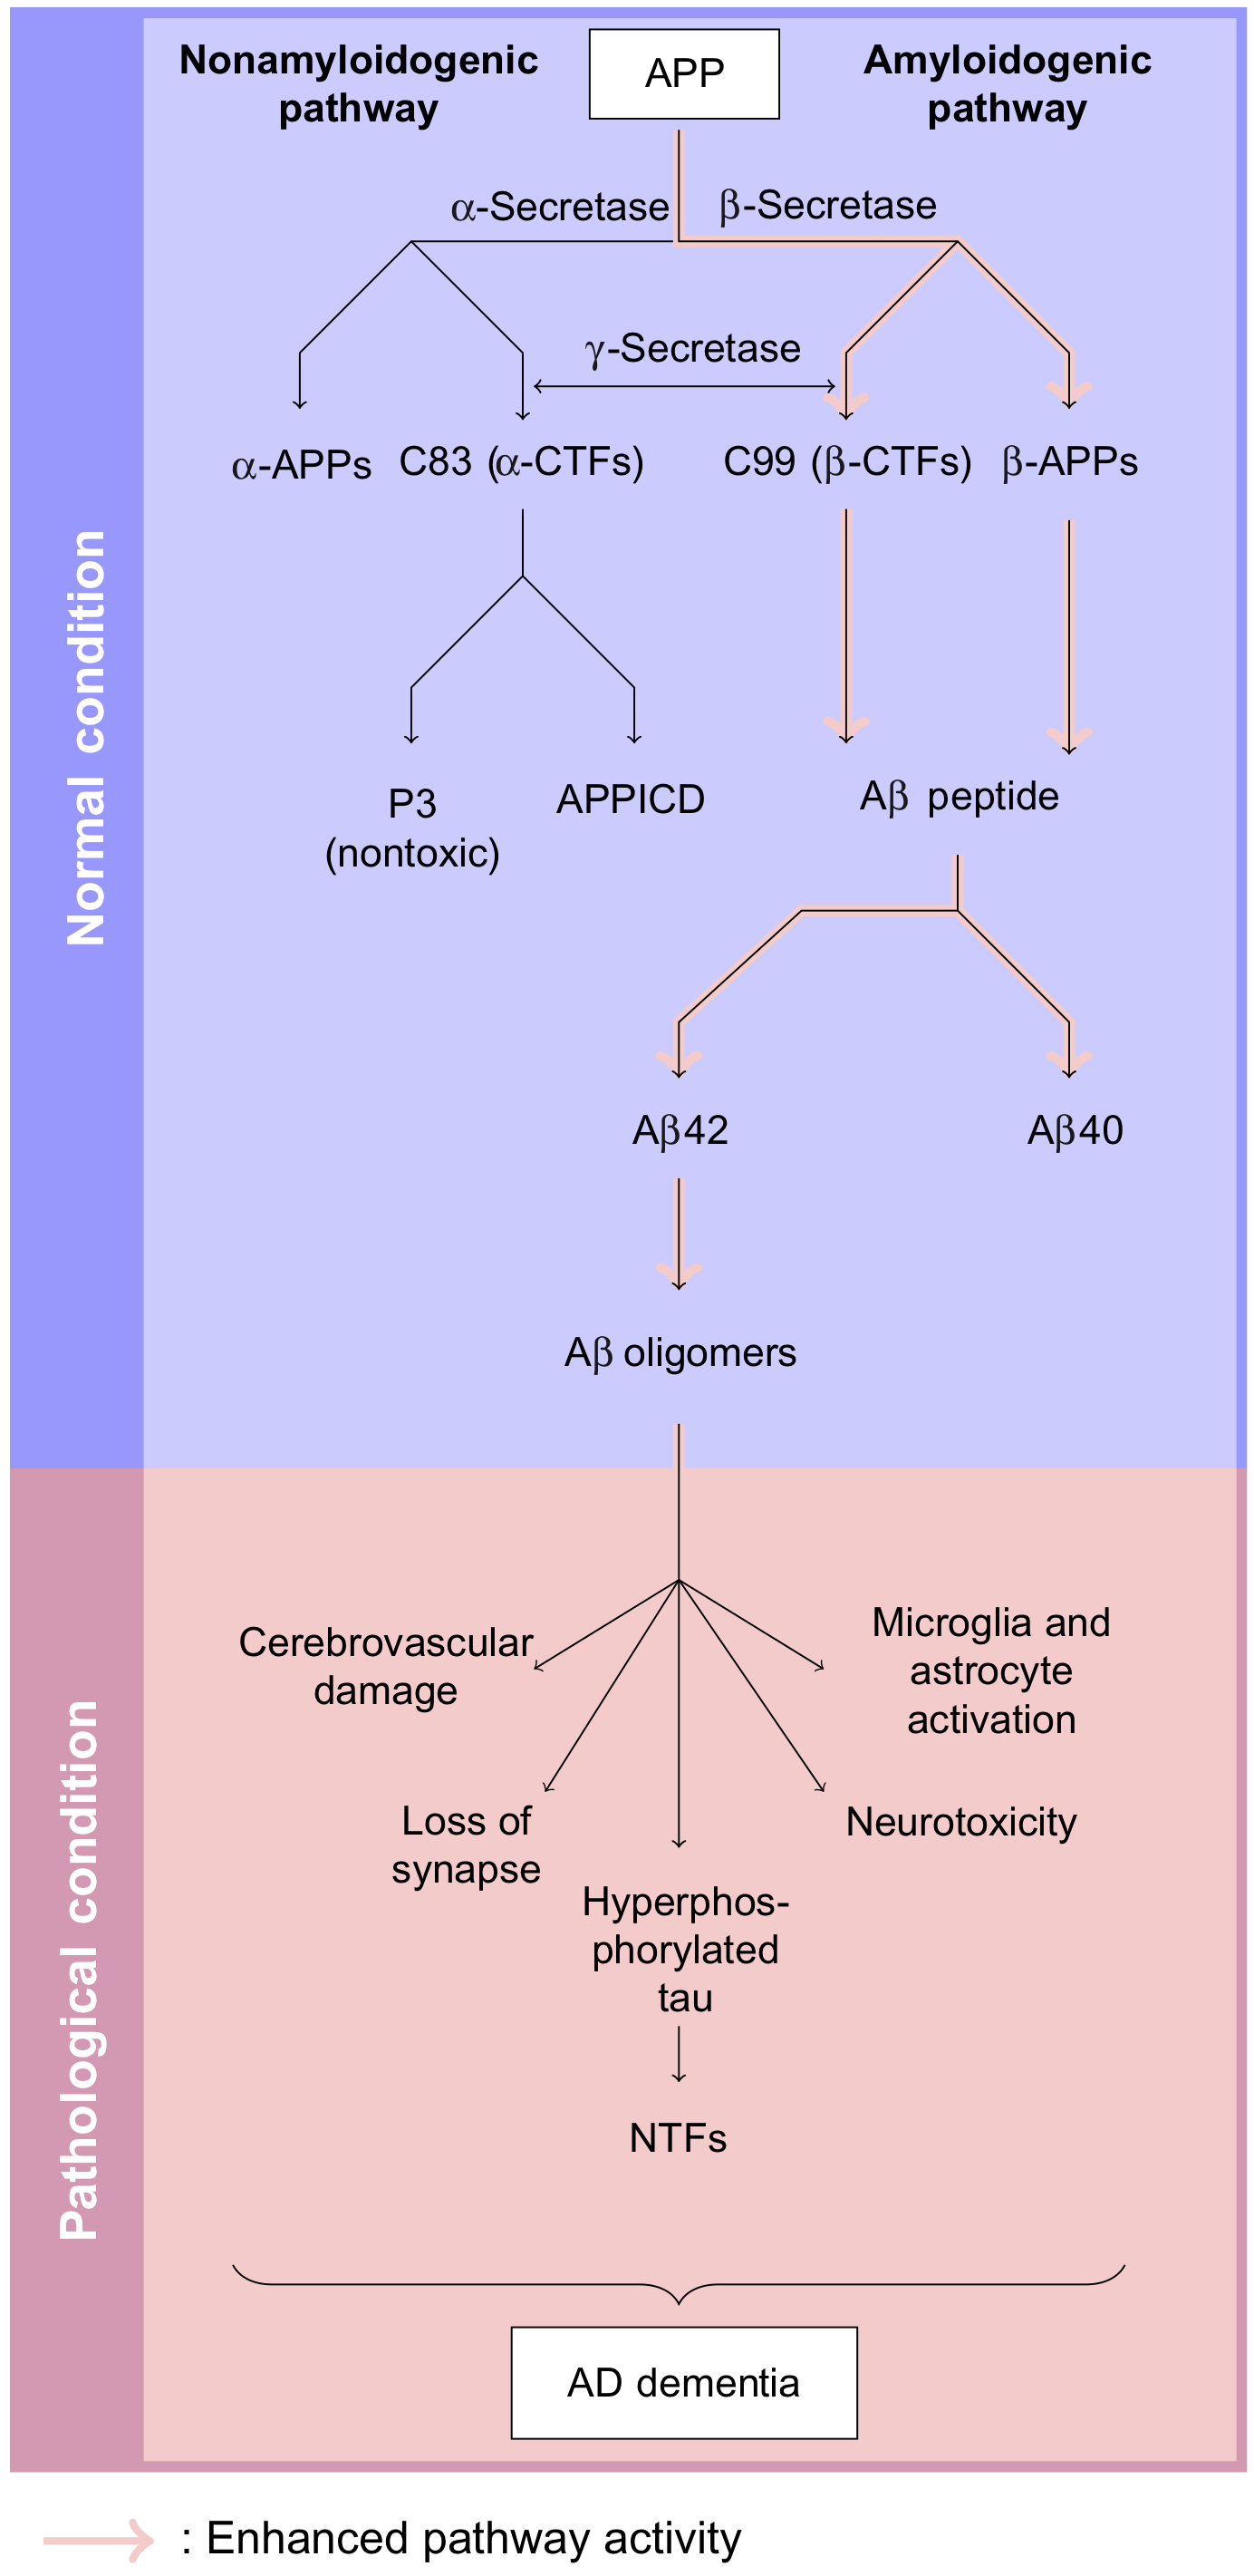
\includegraphics[width=0.7\linewidth]{figures/chapter10/10_amyloidogenic_pathway}
  \caption[The nonamyloidogenic and amyloidogenic pathways.]{The nonamyloidogenic and amyloidogenic pathways. Enhanced amyloidogenic pathway activity increases neuronal synthesis of aggregate prone toxic $A\beta$ oligomers, which in turn lead to autophagy and mitochondrial dysfunction as well as tubulin disruption, thereby driving neurofibrillary tangle (NFT) formation}
  \label{fig:10_amyloidogenic_pathway}
\end{figure}

\section{Advanced microscopy in the study of molecular biology}
\subsection{Role of super-resolution microscopy }

Microscopes play a key role in molecular biology. Fluorescence microscopy in particular remain one of the most important tools for biologists for various reasons. Firstly, it is essential for studying communications of biological molecules inside living cells, tissues, and whole organisms and subcellular structures at high resolution \citep{Han2013}. Secondly, it can acquire data rapidly and molecules of interest are targeted and labelled with specific fluorescence probes in a noninvasively manner \citep{Han2013}. Thirdly, live cell imaging is possible. In conventional microscopes, the spatial resolution is limited in diffraction, about 200 nm in the $xy$ and 500 nm in the $z$ direction, making it impossible to identify smaller sub-cellular structures or monitor biological processes which occur at nanometer scale \citep{Xu2017}. Therefore, in the past two decades, efforts to break the diffraction limit in order to understand cell structure and dynamics at a molecular level, in 2 and 3 dimensions. Currently, super resolution microscopes capable of imaging cellular structures and rapid cellular dynamics at single molecule level at 10 nm are available. These include stimulated emission depletion (STED) microscopy \citep{Klar1999}, saturated structured illumination microscopy (SSIM) \citep{Gustafsson2005}, and single molecule localization microscopy such as  photoactivation localization microscopy (PALM) \citep{Betzig2006} and stochastic optical reconstruction microscopy (STORM) \citep{Huang2008,Xu2017}. STED and SSIM use patterned illumination to improve the resolution by controlling few molecules which are excited and detected simultaneously, while PALM and STORM activate single molecules at different times \citep{Han2013}, \Cref{fig:10_superresolution}. The application of these techniques in molecular biology has been extensively reviewed elsewhere \citep{Han2013}. For the purpose of this review, we focus on single molecule localization techniques.  

Briefly, STORM/PALM is based on the photo switching and detecting single spatially separated fluorophores. This is achieved by photoswitching  fluorophores between their  "ON" and "OFF" state, where most of the fluorophores are forced to remain in the dark state for a longer time and allowing only a small subset of fluorophores  in  the “on” state to emit fluorescence at a given time \citep{Turkowyd2016}. In this manner, thousands of frames are imaged overtime  and reconstructed using image-processing algorithms allowing the precision localization of molecules, which depended on the sufficient collection of photons from each activation event and therefore, the reliability of the fluorophores employed \citep{Turkowyd2016,Xu2017}.

Currently, the use of correlative techniques such as correlative light and electron microscopy (CLEM) is gaining popularity in molecular biology. CLEM is a unique and powerful technique that combines two different imaging modalities, fluorescent light microscopy (LM) and electron microscopy (EM) in order to overcome the limitations of each, however at an expense of imaging fixed sample \citep{Russell2017}. Light microscopy allows one to identify fluorescently labelled molecules for their biological function within living cells and tissues which would not have been possible with EM, however the information is limited in resolution, 200 nm with confocal microscopy and 10 nm with advanced super-resolution microscopy.  EM, particularly the transmission electron microscopy (TEM) allows ultrastructural visualization at a much fine resolution, 0.1 - 10 nm \citep{Feng2018}, thus combining these techniques has makes it possible for imaging rare dynamic biological events at high resolution. Traditionally, CLEM was performed on manually sectioned serial sections and imaging each section (more than 100 sections) using using TEM or SEM (scanning electron microscopy). Nowadays, automated systems  based on the SEM such as focused ion beam SEM (FIB-SEM) \citep{Heymann2006} and serial blockface SEM (SBF-SEM) \citep{Denk2004} have gained popularity and are being used in molecular biology. In FIB-SEM and SBF-SEM, a gallium ion beam  or a diamond knife is used to sputter or remove slices of material from the blockface and the revealed surface is imaged repeated sequentially using a backscattered electron (BSE) detector to build up a stack of images through the volume of the sample \citep{Russell2017}.

\begin{figure}[!htbp]
  \includegraphics[width=\linewidth]{figures/chapter10/10_superresolution}
  \caption[Super-resolution fluorescence microscopy.]{Super-resolution fluorescence microscopy. Diagram showing the principles of super-resolution microscopy techniques (upper panel) and images  of microtubules imaged with each microscopy (lower panel) \citep{Feng2018}.}
  \label{fig:10_superresolution}
\end{figure}

\section{Autophagy}
\subsection{Definition and role}
Autophagy is a major catabolic process responsible for the degradation cytoplasmic material, including organelles within the lysosomal compartment \citep{He2009,Nixon2011}. Three types of autophagy exist, depending on the route through which the encircled cargo is delivered to the lysosomal compartment for degradation: microautophagy, chaperone-mediated autophagy (CMA), and macroautophagy \citep{Boya2013} as shown in \Cref{fig:10_autophagy}. In microautophagy, cytosolic components are directly transferred into the lysosomes through invagination of the lysosomal membrane \citep{Cai2012,Nixon2011}. In CMA, the protein targeted for degradation is recognized by a chaperone complex protein, HSC70, through a KFERQ motif located on the target protein peptide sequence. Subsequently, the substrate-chaperone complex is transported to the lysosome where it binds to the lysosome associated membrane protein type 2A (LAMP2A) receptor allowing the translocation of the protein across the lysosomal membrane into the lumen, where they are degraded \citep{Cuervo2014,Dice2007,Klionsky2010}. And lastly, macroautophagy (here after referred to as autophagy) which is the major degradation pathway of long-lived proteins and organelles, which operates entirely different compared to microautophagy and CMA, through distinct and dynamic membrane rearrangements. Here, a flat membraned cistern known as the phagophore sequesters substrates. The membrane source of phagophores is believed to arise from the  endoplasmic reticulum (ER), plasma membrane, mitochondria and ER-mitochondria contact sites \citep{Hailey2010,Hamasaki2013,Hayashi-Nishino2009,Ravikumar2010,sarkar2013,Yla-Anttila2009}.
The phagophore elongates and encircles the cytoplasmic material, forming a double-membraned vesicle, called an autophagosome \citep{Cai2012,Levine2008}, which subsequently fuses with lysosomes or with late endosomes to form a single-membrane hybrid organelles, amphisome, that latter fuses with lysosomes to form acidic autolysosome \citep{Cai2012,Nixon2011,sarkar2013}, where degradation of the encircled cargo takes place. The resulting macromolecules are recycled back into the cytosol to be reused as substrates for ATP generation or protein synthesis. The rate of protein degradation through autophagy is termed autophagic flux \citep{klionsky2016,loos2014}. Importantly, most cells and tissues have a distinct basal level of autophagic flux \citep{Mizushima2004a}, which has recently been elegantly visualized in various tissues \citep{Kaizuka2016}.  Autophagy therefore plays a critical role in maintaining cellular homeostasis by removing misfolded or damaged proteins and turnover of organelles \citep{Levine2008}. It also plays a role in maintaining energy homeostasis during starvation conditions by recycling cytosolic components to compensate for nutrient scarcity \citep{Levine2008,Loos2009}. Although autophagy play a major role in cellular survival, it has been implicated in various human physiological and pathological conditions, such as development, aging, infection and immunity, longevity, aging, cancer, liver, neurodegeneration and heart disease \citep{Meijer2006,Mizushima2008,Ravikumar2010b,sarkar2013}.

\begin{figure}[!htbp]
  \includegraphics[width=\linewidth]{figures/chapter10/10_autophagy}
  \caption[Schematic representation of the types of autophagy types]{Schematic representation of the three types of autophagy. In microautophagy cytosolic components to be degraded are transferred directly into the lysosome through invagination of the lysosomal membrane, while in CMA, cytoplasmic proteins containing a KFERQ peptide motif are translocated into the lysosomal lumen for degradation. In macroautophagy, cytoplasmic material is sequestrated by an isolation membrane forming an autophagosome, which later fuses with the lysosome to form an autolysosome where degraded takes place \citep{Nikoletopoulou2015}.}
  \label{fig:10_autophagy}
  \end{figure}

\subsection{The autophagic machinery and its regulation}
Autophagy is an evolutionary conserved process from yeast to mammals with up to 36 ATG (autophagy-related genes) \citep{Thumm1994,Tsukada1993,Klionsky2007,Mizushima2010}. Subsets among these ATG proteins referred to as the ‘core’ molecular machinery are essential for autophagosome formation. These are classified into the following groups; (1) the ULK1 kinase complex, (2) ATG9 cycling complex, (3) the class III phosphatidylinositol 3-kinase (P3K)/ Vps 34 complex I, (4) the phosphatidylinositol 3-phosphate (PI3P) binding ATG2-ATG18 complex and (5) ATG12-ATG5 and ATG8/LC3 (microtubule-associated protein 1 light chain 3) \citep{Feng2014,Yang2010}. The autophagic pathway can be categorized into the following essential steps: initiation, expansion of the autophagosome membrane, maturation of the autophagosomes, and degradation. Each step requires tight regulation of several, indispensable, ATG genes \citep{Feng2014,Maday2014,Parzych2014}. 

Although autophagy is constitutively kept at low levels, diverse environmental stressors (e.g. reactive oxidative species, damaged organelles and protein aggregation) can act as inducers of this degradative machinery \citep{Mizushima2008}. Starvation is the classic stimulus for autophagy induction \citep{Kuma2004,Mizushima2004a}, allowing cells to respond to nutrient scarcity through increased allocation of amino acids from proteins sequestered as autophagic cargo \citep{Hosokawa2009}. The classical pathway regulating mammalian autophagy involves the serine/threonine kinase, mammalian target of rapamycin (mTOR): mTORC1 and mTORC2, in which mTORC1 negatively regulates autophagy \citep{Guertin2009,Noda1998,Ravikumar2010b}. During conditions of nutrient availability, active mTORC1 phosphorylates Unc-51-like kinase (ULK1), which is sequestered into a complex with the autophagic protein, ATG13, and focal adhesion kinase family interacting protein of 200kDa (FIP200), thereby inhibiting autophagy. In the absence of nutrients, amino acid deprivation, growth factor withdrawal, or treatment with rapamycin, ULK1 phosphorylation by mTORC1 is reduced and the ULK1 complex is activated through auto-phosphorylation, which in turns phosphorylates ATG13 and FIP200.  Activated ULK1 phosphorylates and activates the Beclin1-vacuolar protein sorting 34 (VPS34) complex, which contains Beclin1, VPS34, and Atg14L \citep{Itakura2008}. The activated Beclin1 complex functions as a class III phosphatidylinositol 3-kinase (PI3KCIII), to produce phosphatidylinositol 3-phosphate (PI3P), which in turn provides a platform to recruit PI3P-binding proteins during the nucleation process \citep{Hosokawa2009,Kim2011,sarkar2013}. Atg14L targets the Beclin1/PI3KCIII complex to the specialized subdomain of the endoplasmic reticulum (ER), called the omegasome, which consequently triggers phagophore formation \citep{Axe2008,Matsunaga2010}. Although the Golgi apparatus, mitochondria and plasma membrane may also act as membrane sources for phagophore formation under certain conditions \citep{Axe2008,Ravikumar2010}, a growing number of studies have revealed that phagophores locate between two cisterns of rough ER in starved cells \citep{Hayashi-Nishino2009,Yla-Anttila2009}. In support of this, the omegasome marker protein DFCP1 was found to be localized in delicate membrane tubules extending from the ER, thus making the ER the most likely membrane source for the formation of phagophores \citep{Uemura2014}. Beclin1 has many binding partners such as Atg14L, UV-irradiation- resistance-associated gene (UVRAG), and Bcl2 \citep{He2010}. Two ubiquitin-like conjugation systems: ATG12-ATG5 and ATG8/LC3 are involved in the elongation and expansion of the phagophore membrane. In the first conjugation system, ATG7 (E1 ubiquitin-activating enzyme-like) activates ubiquitin- like protein ATG12 \citep{Ohsumi2001,Ohsumi1998}, which is then transferred to ATG10 (E2 ubiquitin-conjugating enzyme-like), and eventually conjugated to ATG5 \citep{Geng2008}. The ATG12–ATG5 conjugate interacts with ATG16L1 forming the ATG12–ATG5 –ATG16L1 complex, which is required for the elongation of pre-autophagosome structures, but detaches following autophagosome formation \citep{Mizushima2003}. The second system involves the conjugation of microtubule-associated protein 1 light chain 3 (LC3) to phosphatidylethanolamine (PE). LC3 is processed at the c-terminus by ATG4, to form cytosolic LC3 I, which is converted to LC3 II (membrane bound) when conjugated to phosphatidylethanolamine (PE) in a reaction involving ATG7 (E1-like) and ATG3 (E2-like) \citep{kabeya2000,Tanida2004}. LC3 II specifically associates with the inner and outer surface of the autophagosome membrane, where it is either degraded upon fusion with lysosomes or removed through deconjugation and recycled \citep{kabeya2000,Mijaljica2012,Tanida2004}. Importantly, LC3 II protein levels correlate well with the number of autophagosomes present in the cytoplasm and are hence a key indicator of autophagy or the present autophagosome pool. Although LC3 levels correlate with autophagosome numbers, it is critical to monitor the rate of protein degradation through autophagy, i.e., autophagic flux, through the entire pathway \citep{klionsky2016,loos2014}. 

Following formation, autophagosomes undergo a maturation process that includes fusion with endosomal and lysosomal vesicles \citep{Eskelinen2005}. Studies show that undisturbed autophagic flux requires a tight cooperation between the endosomal compartments, including early- and late endosomal sorting/maturation, and autophagosomes \citep{Eskelinen2005}. For instance, before fusing with lysosomes to form autolysosomes, autophagosomes can also directly fuse with early and/or late endosomes, to form hybrid structure called amphisomes, which then fuse with lysosomes, thereby forming autolysosomes in which the cytosolic content is degraded \citep{Bell2006,Filimonenko2007,Liou1997}. Following degradation, amino acids and nutrients are released back to the cytosol by permeases located on the autolysosomal membrane \citep{Loos2013} Although the degradation of autophagic cargo is non selective, autophagy can also occur in a selective manner. For example, in a selective autophagy, sequestersome 1/SQSTM1 (p62) behave as an adapter protein for LC3-II, resulting to both being degraded \citep{Klionsky2005,Singh2011}. Thus, both p62 and LC3 are used to measure autophagic activity. 

\subsection{Autophagy in healthy neurons – characterized by highly efficient autophagy}
In healthy neurons, autophagosomes are present at low levels \citep{Boland2008,Mizushima2004a,Nixon2005}. These findings initially led to the assumption that there is limited autophagic activity in neuronal cells. It is now, however, widely accepted that autophagy is constitutively active and highly efficient in neurons. This is supported by findings where high numbers of autophagosomes were observed in cultured primary neurons when their clearance was blocked through the inhibition of cathepsins \citep{Boland2008}. This rapid accumulation of autophagosomes occurred without interfering with autophagy induction, supporting the notion that autophagy is constitutively active and that the high clearance rate of autophagosomes keeps their numbers low, manifesting in a small autophagosomal pool size. Indeed, the inherent and tissue-specific \citep{Mizushima2004a} autophagosome synthesis and degradation rate determines the intracellular abundance of autophagosomes, i.e. the autophagosomal pool size, and the extent of autophagosome accumulation (\Cref{fig:10_flux}: \textbf{A}). Scarcity of autophagosome presence in neurons could be brought about by the high rate of both the synthesis and the degradation, if the system is maintained in a steady state with a small autophagosome pool size (\Cref{fig:10_flux}: \textbf{B}\textit{i}, \textbf{C}\textit{i}). However, low levels of autophagosomes may also be due to a decreased synthesis rate or enhanced degradation rate, which is especially the case if the system is in a transition to a new steady state (\Cref{fig:10_flux}: \textbf{C}\textit{ii}, \textbf{C}\textit{iii}). Presence of an autophagosome pool, whether in small or large size, does not necessarily indicate functional autophagy, since only autophagic flux, the rate of protein degradation through autophagy, indicates the function and efficiency of this process. In fact, autophagic flux may be increased with a high or low autophagosome pool size; likewise, flux can be decreased with a high or low autophagosomal pool size \citep{loos2014} (\Cref{fig:10_flux}: \textbf{B}, \textbf{C}). Hence care must be taken when assessing autophagy, since the autophagosome pool size does not dictate the flux, nor vice versa. Despite these observations, the exact autophagosomal pool size and autophagic flux remains largely unknown not only for different subsets of neurons such as in the distinct layers of the cortex, but also for different brain regions that are clinically relevant. The same applies to other types of cells and tissues, such as terminally differentiated cardiac myocytes or proliferating cells; emphasizing the need for a precise cell- and tissue-specific autophagic flux assessment \citep{Kaizuka2016}.

\begin{figure}[h!]
  \center
  \includegraphics[width=0.9\linewidth]{figures/chapter10/10_flux}
  \caption[Flux the rate of flow through the autophagy pathway]{Flux the rate of flow through the autophagy pathway: autophagosome synthesis and degradation rate determine the extent of intracellular autophagosome accumulation (\textbf{A}). When both rates are equal in magnitude, the system is in steady state, characterized by a defined pool size and steady state flux (\textbf{B}\textit{i}, \textbf{C}\textit{i}). The autophagosome pool size can increase due to either enhanced synthesis (\textbf{B}\textit{ii}) or decreased degradation (\textbf{B}\textit{iii}) and can decrease due to dysfunctional synthesis (\textbf{C}\textit{ii}) or enhanced degradation (\textbf{C}\textit{iii}). The autophagosome pool size does not infer flux. }
  \label{fig:10_flux}
\end{figure}

\subsection{Basal autophagy is essential for neuronal homeostasis}
The post-mitotic phenotype of neuronal cells renders them particularly susceptible to the accumulation of damaged proteins and organelles that may have been removed through cell cycle activity \citep{Liang2014,Tan2014}. In order to maintain both cellular and metabolic homeostasis, neurons depend significantly on active basal autophagy to achieve sufficient degradation of functionally redundant proteins and organelles \citep{Meijer2009}, which may be recycled to generate amino acids and ATP. These in turn are anchored in a metabolic feedback loop to regulate autophagic activity and maintain the high energetic demands \citep{Loos2013}. Therefore, the activity of autophagy depends strongly on the metabolic status of the cell. Although neurons depend on autophagy for survival, it has been shown that too much autophagy can be toxic. In support of this notion, multiple studies have shown that high levels of autophagy induced by using Tat-beclin result in cell death in a dose-dependent manner \citep{Liu2013,Liu2015}. However, the flux level at which autophagy becomes detrimental remains to be elucidated. 

Neurons depend highly on autophagy to maintain cellular homeostasis and are characterized by particularly high levels of both ATP demand and protein synthesis \citep{Meijer2009,Son2012}. The latter is indicated by the distinct presence of NISSL substance, composed of abundant rough endoplasmic reticulum (ER), as well as the presence of a dense mitochondrial network. In fact, protein synthesis ranks among the top ATP-consuming processes in the mammalian cell 
\citep{Buttgereit1995}. In addition, tubulin networks and ATP-dependent transport systems control not only autophagosomal but also mitochondrial mobility. This dictates the requirements for a high protein clearance system and a highly functional mitochondrial quality control. During autophagy, autophagosomes are mobilized on their route to degradation by dynein motor proteins that operate along the microtubule network, and are thereby transported towards the perinuclear region, where lysosomes are localized \citep{Fass2006,Jahreiss2008,Kimura2008}. Since many autophagosomes are formed in the synaptic regions, they require efficient transport towards the soma through long neuronal processes for lysosomal fusion. This indicates that the transport process is both timely and energetically more costly than in most mammalian cells. In addition, mitochondria are transported in a similar fashion by utilizing dynein-dynactin complexes, myosin, and kinesin superfamily proteins (KIFs) in order to provide ATP to intracellular areas of high energy demand to maintain neuronal function and survival \citep{Lin2015,Sheng2012}. Hence, functional autophagy is crucial not only for the delivery of proteinaceous cargo, but also for maintaining proteostasis that maintains tubulin functionality. This in turn ensures localized ATP provision that may fuel efficient protein clearance. 

The importance of constitutive autophagy has been elegantly demonstrated in a mouse model, where loss of essential genes, ATG5 or ATG7, resulted in progressive protein aggregation, neuronal loss and neurodegeneration \citep{Hara2006,Komatsu2006}. Conditional knockout of multiple genes, such as ATG3, 5, 7, 9 and ATG16L1, resulted in neonatal lethality \citep{Mizushima2010}. Taken together, these studies demonstrate the critical role of basal autophagy in neuronal homeostasis, metabolism and cell survival. 

\subsection{Neuronal autophagy and aging}
It is widely accepted that the activity of both autophagy as well as CMA deteriorates with age \citep{Cuervo2005}. Indeed, a decrease in autophagy and CMA activity was proposed as one of the major contributing factors in AD \citep{Cuervo2005}. This is evident by the accumulation of cytoplasmic protein aggregates in this disease. However, the extent to which CMA and autophagic flux are affected differentially and region-specifically (\Cref{fig:10_brain}) remains unclear. The model of senescence-accelerated mouse- prone 8 (SAMP8), a rodent model with accelerated aging, revealed deficits in learning and memory with increasing age, characteristic to humans and patients with AD \citep{Ma2011}. Moreover, autophagy dysfunction was indicated by the accumulation of ubiquitin positive proteins in neuronal cells \citep{Ma2011}, supporting the notion that impaired autophagy might contribute to premature aging \citep{Vellai2003}. In support of these findings, studies by \citet{Lipinski2010} revealed down regulation of ATG5, ATG7 and BECN1 in the brains of aging individuals in comparison to their young counterparts. Although CMA-associated protein translation, synthesis and targeting of LAMP2A) remains unchanged throughout life, a drastic change in the stability of this protein with age has been reported due to changes in lipid content \citep{Cuervo2014}. One of the major reasons for reduced CMA degradative activity with age is the dramatic decrease in the lysosomal removal of damaged proteins and organelles \citep{Massey2006}. Although studies have provided evidence of a tightly controlled link between aging, autophagy and CMA, it remains to be elucidated whether the aging process and its associated molecular events have an impact on the autophagy or CMA machinery or whether decreased protein degradation activity accelerates age-related processes. It is also unclear whether autophagic flux in fact decreases or whether a residual heightened flux remains until the onset of neuronal cell death. Further studies are required that assess both autophagic flux and CMA activity in the process of aging. 

\begin{figure}[!htbp]
  \center
  \includegraphics[width=\linewidth]{figures/chapter10/10_brain}
  \caption[Protein aggregation categorized according to Braak staging]{The extent of protein aggregation in the degenerating brain can be categorized according to Braak staging: protein inclusion distribution is characterized by Braak stages I–VI, with progressive protein aggregation in the transentorhinal region, the hippocampus and amygdala and finally the cerebral cortex (top left to bottom right) (\textbf{A}). Spatiotemporal autophagy dysfunction and proficiency failure leads to subsequent protein aggregation. Braak stages I–VI indicating decreasing (left) and increasing (right) region-specific neuronal autophagic flux. To what extent brain susceptibility regions for protein aggregation correlate with either enhanced or diminished autophagic flux remains to be elucidated. The coloured areas indicate highest (red) to lowest (blue) autophagic flux regions a hypothetical cartoon (\textbf{B}).}
  \label{fig:10_brain}
\end{figure}

\section{Autophagy dysfunction in AD}
\subsection{Brain autophagy flux differs regionally}
Autophagic flux and its response to specific stimuli are distinct and differ across the regions of the cerebrum. Previous studies revealed differences in the autophagy response to caloric restriction in Purkinje cells compared to a specific subset of neurons in the cerebral cortex \citep{Alirezaei2010}. Purkinje cells were, in particular, lost upon ATG knockout, supporting the notion of regional autophagic flux differences \citep{Alirezaei2010,Hara2006,Komatsu2006}. Yet, the fusion ability of autophagosomes with lysosomes was not assessed in these scenarios by using either BafA1 or chloroquine, which makes interpretation of autophagic flux challenging. Similar results were reported in a study where exercise robustly induced autophagy in the cerebral cortex of adult mice, but not in other brain regions such as the hypothalamus, midbrain or cerebellum \citep{He2012}. It is unclear which parameters control these characteristics and the question of autophagic flux differences in respective brain regions has received relatively minor attention in the literature. By using laser capture microdissection, recent work supports the notion of brain region-specific autophagy. Here, it was elegantly shown that not only is the autophagic machinery differentially impacted between CA1 (Cornu Ammonis 1) pyramidal hippocampal neurons and glial cells from AD subjects, but also that autophagy if competent and upregulated, yet with progressively deficient cargo substrate clearance \citep{Bordi2016}. Even though it is not fully understood how autophagic flux differs across the brain, it becomes increasingly clear that autophagy regulation is organ- and tissue-specific. Skeletal muscle, pancreas and heart expressed high levels of LC3-II followed by kidney and liver, and lastly the brain with limited expression of LC3-II \citep{Mizushima2004a}. In this study the presence and abundance of LC3-I may be of importance, since it may indicate the cytoplasmic availability of LC3, and therefore the ability to generate autophagosomes rapidly. The brain has been indicated with highest levels of LC3-I, suggesting major ability to respond rapidly with a change on autophagosomal pool size, without necessarily requiring de novo LC3 synthesis \citep{Mizushima2004a}.

It is known that neurodegenerative diseases affect defined loci and anatomical regions in a distinct manner with a specific and time-dependent manifestation of protein aggregation \citep{Wang2010a,Wang2010b}. In AD, for instance, so-called susceptibility regions are affected in a cumulative manner, characterized by a particular spatiotemporal protein aggregation profile classified as Braak staging (\Cref{fig:10_brain}: A). This system, which has recently also been expanded to Parkinson’s disease (PD) \citep{Braak2004}, refers to an approach formulated in 1991 by Braak and Braak for staging the severity of AD, based on the premise that its pathology, specifically neurofibrillary tangles, evolves in stages and manifests in defined anatomical locations. The disease begins in the mesial temporal lobe (stages I and II) and extends to the limbic regions (stages III and IV) at which point dementia finally manifests clinically, with tangles also present in the neocortex (stages V and VI) \citep{Braak1991}. Hence, the staging can be utilized to characterize protein aggregation in AD pathology. In brief (\Cref{fig:10_brain}: A), stage I primarily affects the trans-entorhinal region, while stages II and III primarily affect defined regions of the hippocampal formation such as the entorhinal region, CA1 and the subiculum \citep{Braak1991,Braak2012}. Stage IV, however, affects CA4, the fascia dentata (FD) and the amygdala, while stages V and VI affect the entire hippocampal formation and isocortical areas \citep{Braak1991} (\Cref{fig:10_brain}: \textbf{A}). 

Besides the differences in affected regions, AD does not affect neurons equally in the same regions \citep{Wang2010a,Wang2010b}. In the hippocampal formation, for example, neurons in the layer II of the entorhinal cortex are most susceptible to protein aggregation, followed by neurons in the CA1, subiculum \citep{Wang2010a,Wang2010b}, and CA4 region, while neurons in the CA2 and CA3 are the least vulnerable \citep{Schonheit2004,Wang2010a,Wang2010b}. In addition, neurons in the hippocampal formation are more susceptible to protein aggregation compared to neurons in the cerebral cortex which show an aggregate-prone phenotype later in the disease stage. It may be speculated that this selective vulnerability indicates inherent differences in the rate of protein degradation through autophagy, and potentially characterizes neuronal dependency on autophagic flux (\Cref{fig:10_brain}: \textbf{B}). Hence neurons in the defined regions may be characterized by the highest aggregate-prone phenotype due to their inherent reliance on autophagy (\Cref{fig:10_brain}: \textbf{B}). For example, neurons in the brain region affected during stage I might be more dependent on autophagic flux, with high basal rates, compared to those affected during stages II and III (\Cref{fig:10_brain}: \textbf{B}, Left). Here, autophagy dysfunction would lead to a rapid aggregation of toxic protein species. 

In fact, the relationship between proteostasis and neurodegeneration has previously been elegantly indicated at the single- cell neuronal level by assessing the half-lives of mutant huntingtin protein \citep{Tsvetkov2013}, suggesting that autophagic flux may indeed predict neuronal vulnerability to protein-prone aggregation. Recent work assessing the autophagy profile in CA1 pyramidal neurons supports the notion of cell and region-specific autophagy activity and vulnerability to substrate clearance \citep{Bordi2016}, suggesting that such a scenario is indeed mirrored in an \textit{in vivo} setting. It is also plausible that neurons affected during stage I might be characterized by the lowest level of basal autophagic flux compared to those neurons affected by later stages and hence may manifest first with an aggregate-prone phenotype, since the ability to degrade protein species is inherently limited (\Cref{fig:10_brain}: \textbf{B}, Right). The latter speculation is supported by recent findings suggesting that protein turnover indeed differs substantially between neurons (Mitra et al., 2009). Indirect evidence is also provided by ATG7-deficient mouse brains that are characterized by distinct region-specific p62/SQSTM1 protein levels that appear low in the hippocampal and amygdala region and high in the cerebral cortex \citep{Komatsu2007}. Since p62 is a multifunctional LC3 binding protein that is degraded with a particular cargo, its aggregation is an indication of decreased autophagic activity \citep{Komatsu2007}. Further research is required to enhance our understanding in region-specificity with regard to autophagic flux, susceptibility to aggregate formation and proteotoxicity. This could provide insight into novel and more precise targets for protein aggregate clearance to maximize the effectiveness for therapeutic interventions. 

\subsection{Autophagy defects are diverse and distinct - a need for precision targeting}
It is becoming increasingly clear that an autophagy defect is one of the key molecular mechanisms and contributing factors for the development of AD (\Cref{fig:10_autophagy_progression}) \citep{Nixon2005,Nixon2011}. The autophagy process can mechanistically be described by several defined stages including the induction, elongation (cargo recognition), maturation, fusion and degradation. AD is often characterized by particular molecular defects that manifest not only in different compartments of the autophagic machinery but also with distinct subtypes of autophagy being affected (\Cref{fig:10_autophagy_progression}). Defects have been suggested in the induction step, autophagosome maturation as well as in the degradation step of the pathway. Beclin 1, an autophagy initiator, which serves in the anchoring and recruitment process of autophagy-related proteins essential for the induction and elongation of autophagosomes, has been reported to be reduced in brain tissue derived from AD patients, particularly in the early stages of the disease \citep{Pickford2008}. It has been suggested that loss of the Beclin 1 encoding gene (BECN1) impairs autophagy \citep{Frake2015,Pickford2008}, thus impairing autophagosome formation. In line with these findings, knockout of Beclin 1 has been shown to result in increased accumulation of $A\beta$ in APP transgenic mouse models \citep{Pickford2008}.

A defect in autophagosome clearance was initially suggested in studies by \citet{Nixon2005} and \citet{Boland2008}, where autophagosomes filled with undigested material were found to accumulate in affected neurons. It was suggested that mutations in PS1 contribute to impaired autophagosome clearance due to its function in lysosomal acidification and the fusion of lysosomes with autophagosomes \citep{Lee2010,Neely2011}. These studies support the notion of lysosomal failure in the pathogenesis of AD, which had been indicated prior to the identification of autophagic dysfunction. Similarly to AD, Niemann-Pick type C disease, which is classified as a tauopathy, also leads to an accumulation of autophagic vacuoles in neurons. Here, impaired autophagic flux resulting from dysfunctional autophagosomal-lysosomal degradation has been reported \citep{Elrick2012,German2001,Meske2016}. It is thought that the mutation in the NPC1 gene results in disturbance in the trafficking of cholesterol within the cell, leading to a build- up of unesterified cholesterol and glycosphingolipids in the late endosome/lysosome compartment \citep{Elrick2012,Meske2016,Nixon2004}. The nature of the lysosomal membrane is crucial here, since it may have an impact not only on the lysosomal acidification process and hence degradative function but also on the multimerization of membrane proteins and the recruitment of SNARE (soluble N-ethylmaleimide-sensitive factor attachment protein receptor) proteins that drive and regulate the fusion process \citep{Itakura2012}.

Evidence highlighted above suggests that autophagic dysfunction manifests with a distinct molecular profile which may be localized upstream or downstream of the autophagic machinery. This demand matched molecular precision control to re-establish autophagic pathway activity. In fact, the pharmacological target as well as dosing and scheduling of the intervention will have a significant impact on the disease outcome and deserves further study. A mere increased initiation of autophagy may indeed be detrimental if the clearance is defective. A therapeutic strategy would have to alleviate any lysosomal defect, re-establish lysosomal acidification followed by the induction of autophagy. Here, nanoparticles may form part of the treatment regimen, to target the lysosomal compartment to enhance re-acidification \citep{Peynshaert2014}. However, enhancing autophagy and protein clearance may be beneficial to one subset of neurons, while detrimental to another, where lysosomal dysfunction has already advanced, further supporting the notion of isolating autophagy cargo and machinery defect. Measures of autophagosome flux \citep{loos2014} and levels of autophagic activity \citep{Kaizuka2016} in conjunction with measures of the aggregate-prone protein species levels will be crucial to developing suitable and aligned targeted interventions.

Although a decline in autophagic flux is one of the key molecular mechanisms contributing to the development of neuronal dysfunction, multiple studies have reported its temporary increase at the disease onset. This suggests that autophagy requires to be assessed during various stages of the pathogenesis. For example, previous studies have reported an increase in autophagic flux after amyloid beta stimulation in transgenic mouse models of AD \citep{Hung2009,Wang2010a,Wang2010b,Yu2005}. Similar findings have been reported in other diseases such as HD and PD. For example, high levels of autophagic flux markers were observed in mouse models of HD and brain tissue derived from patients \citep{Heng2010,Nagata2004,Ravikumar2004}. In PD, mutations in a-synuclein (A53T and A30P), DJ1 and PINK1 have all been implicated in the increase of autophagic flux \citep{Irrcher2010,Michiorri2010,Plowey2008,Stefanis2001}, leading to the shrinkage of neurites. These data point towards the role of autophagy to serve as initial stress response \citep{Loos2009} in an attempt to clear toxic protein aggregates. It remains to be elucidated whether the increase in autophagic flux is due to a change in aggregate-prone protein levels or metabolic perturbations, or whether it is a correlative effect of other signalling events implicated in the cellular stress response. Common in the above scenarios is the progressive increase in the accumulation of aggregate-prone proteins, despite an autophagy response. When enhanced autophagy starts to fail or overburdens dysfunctional lysosomes \citep{Bordi2016}, and whether increased autophagic flux in fact remains elevated in the different disease conditions, remain to be elucidated and deserve further study.

\begin{figure}[!htbp]
  \includegraphics[width=\linewidth]{figures/chapter10/10_autophagy_progression}
  \caption[Diverse and distinct autophagy defects]{Autophagy defects are diverse and distinct: diagram depicting the progression of autophagy from induction of autophagosome formation to their elongation, maturation and fusion with lysosomes, followed by degradation and recycling. Distinct molecular defects in the autophagic pathway are associated with the onset of Alzheimer’s disease (AD), resulting in dysfunction in autophagy induction, autophagosome maturation and clearance or cargo recognition.}
  \label{fig:10_autophagy_progression}
\end{figure}

\section{Autophagic flux control}
\subsection{Assessment of the autophagic machinery}
Many tools and techniques exist in the assessment of autophagy \citep{klionsky2016}. However, measuring autophagic activity remains complex and challenging. In healthy neurons, basal autophagy is commonly studied by incubating cells first under nutrient rich conditions in the presence of serum-supplemented medium. Autophagy can then be induced by maintaining cells under stress conditions such as nutrient deprivation \citep{Alirezaei2010}, hypoxia and ROS, or by treating cells with pharmacological agents such as rapamycin or other autophagy-inducing compounds \citep{Boland2008,Rose2010}. This is usually performed in the presence and absence of either autophagosome formation inhibitors (3-MA, LY294002) or, and most commonly so, lysosomal fusion inhibitors (leupeptin, chloroquine, BafA1). Subsequently, relative changes in autophagy-related proteins, in particular LC3, are assessed; these would be indicators for autophagic flux. The autophagic machinery is usually assessed using various methods, including TEM to visualize the ultrastructure of the autophagic machinery components and its pathway entities, i.e. autophagosomes, lysosomes and autolysosomes \citep{klionsky2016}. In conjunction, western blot analysis is usually performed for the quantification of autophagy-related protein levels such as LC3-II and sequestosome 1/SQSTM1 (p62) and is often accompanied by fluorescence microscopy-based techniques for the visualization and quantification of LC3 and p62 positive structures \citep{klionsky2016,Klionsky2012,Mizushima2007,Swanlund2010}.

While techniques to monitor the autophagy machinery \textit{in vitro} are relatively advanced, methods to assess this process \textit{in vivo} are less developed and remain a major challenge. An \textit{in vitro}-based approach favors the implementation of various molecular techniques such as transfections, live cell imaging, quantitative morphometric analysis, and the dynamic assessment of key autophagy proteins involved. Nonetheless, it is possible to monitor the autophagic machinery \textit{in vivo} by assessing GFP-LC3 using fluorescence microscopy, and p62 by immunohistochemistry and/or western blot analysis \citep{klionsky2016}. Models to assess autophagy \textit{in vivo} include the use of wild type or transgenic mice expressing GFP-LC3 \citep{Mizushima2004a,Rodriguez-Muela2012}, or in animals transfected with GFP-LC3 plasmid \citep{Mammucari2007}. Early work by \citet{Mizushima2004a} revealed that autophagy is differentially induced in tissues using transgenic mice expressing GFP-LC3. In line with these findings, previous work has shown differential regulation of autophagy in tissues, with the liver exhibiting high autophagic activity compared to the spleen \citep{Haspel2011}. Furthermore, other studies have monitored changes in autophagy in skeletal muscle and the heart after treatment with colchicine \citep{Ju2010} or chloroquine \citep{Kanamori2015}. The recent development of the ratiometric flux probe GFP-LC3-RFP-LC3$\Delta$G has demonstrated for the first time the successful assessment of autophagic activity \textit{in vivo} \citep{Kaizuka2016}. Here, a ratiometric assessment using intensity look up tables indicates visually regions of high or low autophagic activity. However, autophagic activity measured in the entire mammalian brain is yet to be accomplished. In addition to using transgenic models to monitor autophagy \textit{in vivo}, immuno-histochemical staining is a feasible avenue. This technique is advantageous since it can be employed in studies using postmortem human tissue. Immunodetection of LC3 and p62 punctate can be performed in paraffin-embedded tissue sections and fresh frozen tissue using immunohistochemistry or immunofluorescence \citep{He2016,Holt2011,Martinet2006,Schlafli2015}. These methods however do not lend themselves well to a dynamic assessment \citep{klionsky2016}.

In contrast to assessing autophagy \textit{in vivo}, it is possible to assess autophagy in tissues ex vivo. This approach eliminates the risk of toxicity and bioavailability of compounds such as BafA1, leupeptin, colchicine and chloroquine; which are problematic in animal studies. Using ex vivo methods, autophagy has been monitored in retina \citep{Esteban-Martinez2015} and organotypic cultures in the presence of protease inhibitors. This method allows FACS (fluorescence-activated cell sorter) based techniques to be employed in addition to western blotting and fluorescence microscopy. Due to the technical limitations in performing real time analysis in animals, autophagy assessment \textit{in vivo} is usually limited, and techniques are most often executed at a single time point only, following the exposure to suitable inhibitors. Such approach is thereby providing a measure of basal or induced autophagy flux, assessing whether flux remains unchanged, is increased or decreased. Nevertheless, attempts to quantify respective protein levels over time, and assessing the slope of plotted LC3 protein levels as a measure for autophagosomal accumulation, have revealed fundamental aspects of tissue specific autophagic flux \citep{Haspel2011} (\Cref{fig:10_flux_tissue}: A), since they are inclusive of the dynamic changes in time and mirror advances in \textit{in vitro} methods. In that way it was recently revealed that the liver and the heart have the highest autophagic flux, while the kidney, spleen and lung are characterized by a lower flux, indicated by levels of LC3-II \citep{Haspel2011}. However, the inherently high degree of variability in western blot analysis and the reference from LC3 protein levels to autophagosome pool size create additional challenges for a standardized approach to measure autophagic flux \textit{in vivo}. Real time and multi-scale tissue imaging, such as light sheet microscopy \citep{Pampaloni2013}, will undoubtedly contribute to the improvement of future autophagy flux analyses, providing the opportunity to implement morphometric approaches to quantify autophagic flux and pool sizes (\Cref{fig:10_flux_tissue}: \textbf{B}). 

\begin{figure}[!htbp]
  \includegraphics[width=\linewidth]{figures/chapter10/10_flux_tissue}
  \caption[Assessment of the autophagic flux in tissues.]{Assessment of the autophagic flux in tissues - a complementary approach.(\textbf{A}) Tissue isolated from different brain regions in the presence and absence of BafA1 is collected over time and the change in LC3-II protein levels is assessed using western blot analysis. (\textbf{B}) Cells isolated from brain regions are prepared for single cell pool size and flux analysis. The complete pool size of autophagosomes is quantified using live cell fluorescence microscopy and image morphometric analysis. Following acquisition in the absence of bafilomycin A1 as well as after treatment with saturating concentrations of bafilomycin A1, the progress curve of the autophagosome pool size is plotted (\textbf{B}). Cells are analyzed for autophagosome number nA (green), lysosomes nL (red), and autolysosomes nAL (yellow) and quantified to derive the flux J, expressed as autophagosomes/cell/hour.}
  \label{fig:10_flux_tissue}
\end{figure}

\subsection{Assessment of autophagic flux  toward a standardized characterization}
In the above-mentioned studies, the techniques utilized to assess the autophagic machinery have the potential to evaluate the level of autophagic activity. They are, however, less aligned with the requirements to quantify autophagic flux per se when measurements are based on a single time point. Based on the discussions above, there is an urgent need for a more precise and standardized characterization of autophagic flux, autophagosomal and lysosomal pool sizes so as to unravel the underlying mechanisms that may govern a particular flux status more effectively. \textit{In vitro} methods on single cells are at present most aligned to measure autophagic flux as they allow the accurate count of autophagosomes per cell in time. This method should not be limited to assessing whether or not autophagic flux has changed, but should also report on the magnitude of the flux, when the flux is changing and how long it remains at a given steady state. This requires the use of a technique that allows the inclusion of a time dimension, making it possible to quantify even minor changes in flux, such as a change by 2 \% or 5 \%, reported as autophagosomes/hour/cell. Such a technique would be ideal to provide information about the flux at basal levels, its deviation in pathology, and the potencies of specific autophagy modulators with the aim of offsetting this deviation. 

We and others have recently shown that the autophagic system can be treated as what it is: a multistep pathway where there is a rate of flow of material of which each step is characterized by a particular rate \citep{Meijer2009,loos2014}. We have proposed a technique in which autophagic flux and other entities can be measured \textit{in vitro}. This technique, which is extensively described elsewhere \citep{loos2014}, may be adapted ex vivo, for example, by using transgenic fluorescence model systems \citep{Mizushima2004a} to isolate cells of interest (\Cref{fig:10_flux_tissue}) or by using PBMCs isolated from patients \citep{Rangwala2014} to allow an indication of systemic autophagic flux. When combined with microdissection, susceptibility regions may be assessed in that manner (\Cref{fig:10_flux_tissue}: \textbf{A}) to complement other techniques that assess autophagy. Cells must, however, be treated with saturating concentrations of BafA1, so as to minimize remaining residual flux, and imaged at multiple time points to reveal the autophagosome pool size, autophagic flux and transition time. In doing so, it becomes clear that autophagosome pool size does not infer autophagic flux (\Cref{fig:10_flux} and \Cref{fig:10_flux_tissue}). In fact, neuronal cells are, in particular, characterized by a small pool size nA and a high flux J. Knowing and assessing these parameters will not only allow a robust comparison of autophagic flux between neuronal cells in different brain regions as well as within distinct nuclei, but it will also be possible to compare differences in autophagic flux under physiological conditions as well as degenerative disease states. Finally, it will enable a precise modulation of autophagy using pharmacological agents or lifestyle interventions in order to clear protein aggregates. In doing so, the transition time required to turn over the autophagosome pool can be correlated to particular candidate protein species that show aggregation, aligning them with a favorable autophagic flux for their clearance. Future work that focuses on the use of high content screening systems in this context will undoubtedly advance our ability to better control and manipulate autophagic flux. 

Recently, more direct methods to infer autophagic flux have been implemented through the use of photoactivatable or photo- switchable proteins to monitor the decay of fluorescence signal of reporter proteins linked to LC3 protein (e.g. Dendra2-LC3) over time, allowing the determination of half-lives for specific proteins \citep{Tsvetkov2013}. This method also makes it possible to correlate autophagic flux with the rate of the cargo protein degradation. Taken together, a combination of dynamic techniques such as the autophagosome flux assessment together with cargo protein photoactivation and western blot analysis over time will allow robust measures of the rate of protein degradation through autophagy.

\section{Autophagy modulation in therapy-achieving flux control}
Given the important role of autophagy in cell survival and its involvement in neuropathology, there has been a growing interest in manipulating this pathway as a potential therapeutic target for AD (Table 1 and 2). Multiple studies have shown that induction of autophagy via mTOR dependent and mTOR independent pathways using pharmacological agents reduces aggregate prone proteins and associated disease pathology in models of AD. However, major deviation exists between experimental design, drug concentrations utilized, duration of treatment intervention as well as the model system employed to assess autophagic flux (Table 1 and 2). In this section we highlight the wide range of autophagy modulating drugs so as to draw attention to the requirement to achieve better flux control. Given the dynamic and tissue-specific nature of autophagy, implementation of a sensitive and standardized measurement approach will be beneficial in unravelling underlying autophagy flux deviations and in aligning treatment strategies.


\begin{landscape}
\begin{table}[p]
\centering
\caption[]{}
\label{}
\begin{tabular}{lllllp{5cm}lllllll}

\toprule
& Autophagy modulators & FDA & Disease model & Mutant protein & Brain region (cell type) & Dose & Duration & Basal flux & Induced flux inhibition & Assessment for aggregation & Assessment for autophagy & References \\
\midrule
 & Rapamycin & Yes & AD  & Tau & Eyes & 1 $\mu$M & - & - & - & LM  (Tau) & - & \citep{Berger2006}\\
mTOR dependent &  &  &  & APP & Hippocampus & 2.24 mg/kg & 1x per day for 13 weeks & - & - & WB (A$\beta$40/ 42, APP),  Elisa (A$\beta$40/42) & WB (LC3II \& p62), FM (LC3 II) & \citep{Spilman2010}\\
 &  &  &  &  PS1M146V/APPswe/Tau P301L & Cortical areas  (peri-rhinal cortex) Hippocampus (CA1 pyramidal neurons) & 14 mg/kg & everyday for 3 and 16 months & - & - & WB (APP), FM, LM \& ELISA (AB40/42), LM \& WB (Tau) \& WB (APP, C99, C88 \& tau) & WB (LC3 II,  ATG7, ATG 5/ ATG 12), EM (Autophagosomes) & \citep{Majumder2011}\\
 &  &  &  &  PS1M146V/APPswe/Tau P301L & Hippocampus (CA1 pyramidal neurons) & 2.24 mg/kg & everyday day for 10 weeks & - & - &  ELISA (AB40/42), WB, FM, LM \& ELISA (Tau) \& WB (APP, C99, C88 \& tau) & WB (LC3 I, II, ATG7, ATG 5/ ATG 12) & \citep{Caccamo2010}\\
mToR independent & Lithium & Yes & AD  & Tau P301L & Left and right hemisphere \& anterior horn of the spinal cord  & 2 g/kg \& 1g/kg & everyday for 2 months with 2g and everyday for 2 months with 1g (total of 4 months) & - & - & WB \& LM (Tau) & LM \& FM (LC3) \& WB (p62) & \citep{Shimada2012}\\
 &  &  &  & ABPPSWE/PS1A246E  & Cortex \& Hippocampus  & 0.18 mmol &  every day for 3 months  & - & - &  ELISA, FM \& WB (A$\beta$40/42) \& WB (APP, BACE1,C99, C88 \& tau) & WB \& FM (LC3)  & \citep{Zhang2011}\\
 & Carbamazepine & Yes & AD  &  APPswe/PS1deltaE9 & Cortex \& Hippocampus  & 100 mg/ml & per day  & - & - & FM \& LM (A$\beta$), ELIZA (A$\beta$42), WB (APP, BACE1,Alp1a) & WB (LC3 II, p62), FM (LC3) & \citep{Li2013} \\
 & Trehalose & No & Tauophathy  & Tau & Cerebral cortex layer I-III, brainstem e.g pontine nucleus & 0.02 & 2x a week for 4 months & - & - & WB (tau) \& FM (tau, AT100 positive inclunsions) & WB \& FM (LC3 II, p62) & \citep{Schaeffer2012}\\
 &  &  &  &  & Hippocampus, cortex, striatum, sustantia nigra & 0.01 & 2x a week for 2.5 months \& 4 months & - & - & FM, LM (A$\beta$) \& WB (tau) & WB, FM (LC3 II, p62,) \& EM (AVs) & \citep{Rodriguez-Navarro2010}\\
 & Rilmenidine & Yes & HD  & Htt  & Periform cortex, motor cortex \& hippocampus & 10 mg/kg & 4x a week for 24 weeks & - & - & FM \& WB (htt ) & WB (LC3) & \citep{Rose2010}\\
 &  &  & ALS  & SOD1 & Spinal cord e.g spinal motor neurons & 10mg/kg & 4x a week   & - & - & FM \& WB (SOD1) & WB (LC3 II, p62, LAMP2A, VDAC1, HSPA8) \& FM (LC3 \& LAMP2A) & \citep{Perera2018}\\
 & Spermidine & Yes & FLD  & TDP-43  & Cortex \& Hippocampus  & 50 mg/ml & 3x a week for 30 days & - & - & FM (TDP-43) & WB (LC3 II and p62) & \citep{Wang2012}\\
 &  &  & PD  & $\alpha$-synuclein  & Dopaminergic neurons & 5 mM & 24 and 48 h & - &  & WB ($\alpha$-synuclean) & WB (LC3 II) & \citep{Buttner2014}\\
 &  &  &  &  &  &  & - &  &  & FM ($\alpha$-synuclean) &  FM (LGG-1) & \\

\bottomrule
\end{tabular}
\end{table}
\end{landscape}
% add in-text table references

\subsection{mTOR-dependent autophagy control}
Rapamycin was the first drug to be identified as an autophagy enhancer \citep{Blommaart1995,Noda1998}. Rapamycin binds to the cytosolic protein FK506-binding protein (FKBP12) and forms the rapamycin-FKBP12 complex \citep{Cardenas1995}. In turn, this complex blocks the mTOR pathway by interacting directly with mTORC1 \citep{Cardenas1995,Lorenz1995}. Thus, rapamycin up-regulates autophagy by direct inhibition of mTOR, which regulates important cellular functions such as translation of proteins, cell growth and metabolism \citep{Laplante2012,Polak2009}. Rapamycin has been shown to induce autophagy and reduce the levels of mutant tau and $A\beta$42 levels leading to neuronal protection when used at a concentration of 2 $\mu$g/ml for 48 h \citep{Berger2006} and at 0.5, 5 \& 50 $\mu$g/ml for 24 h \citep{Caccamo2010} respectively, in \textit{in vitro} models of AD (Table 1). In APP transgenic mice model, long-term inhibition of mTOR by rapamycin alleviated AD cognitive like deficit and lowered toxic $A\beta$42 levels when administered at concentrations of 2.24 mg/kg per day for 13 weeks \citep{Spilman2010} (Table 2). In another study using 3xTg-AD mice, induction of autophagy with rapamycin at 14 mg/kg for 3 and 16 months resulted in a reduction in amyloid plaques, NTFs, and cognitive defects  \citep{Majumder2011}. Moreover, use of rapamycin at 2.24 mg/kg per day for 10 weeks in a mouse model of AD rescued cognitive deficits and ameliorated tau pathology by increasing autophagy \citep{Caccamo2010}, while its use at 1 $\mu$M decreased tau associate toxicity in flies, likely by mechanisms involving autophagy, however autophagy markers were not assessed \citep{Berger2006}. Rapamycin analog CCI-779 has also been shown to have neuroprotective roles in AD. In HEK 293 cells expressing the Swedish mutant of APP695, CCI-779 was reported to protect cells from toxicity by enhancing the clearance of $A\beta$  through autophagy upregulating when administered at a concentration of 100 nM for 24 h \citep{Jiang2014a}. In APP/PS1 transgenic mice CCI-779 administration at 20 mg/kg every 2 days for 2 months reduced $A\beta$ plaques and alleviated learning and memory deficits \citep{Jiang2014a} by autophagy induction. Despite the promising effects of rapamycin and its analogs in protection against AD related pathology through autophagy induction, these compounds cannot be used in chronic diseases like AD that require treatment for a longer time as they afford protection  by inhibiting mTOR activity essential for protein synthesis. It is also possible that the protective roles of rapamycin and its analogs could also be brought about by mechanisms that occur independent of autophagy, yet initiated by mTOR inhibition. This scenario makes it challenging to interpret results especially in studies of neurodegeneration, where a decline in a toxic protein species could be due to a decrease in overall protein synthesis and not as a result of autophagy induction by rapamycin. Therefore it should be established as to what extent rapamycin decreases overall protein burden or induces autophagy. This could be achieved by inhibiting protein synthesis using cycloheximide \citep{Watanabe-Asano2014} followed by assessing markers of neuronal protection. While inhibition of protein synthesis may serve as a suitable control \textit{in vitro}, this method might have detrimental side-effects \textit{in vivo} and requires further investigation. In addition to regulating protein synthesis and autophagy, rapamycin is an immunosuppressant \citep{Khanna2000,Mohacsi1992,Wicker1990}. Since AD include important neuroinflammatory components, rapamycin could also result in improvement by decreasing neuroinflammation. Previous studies have shown that rapamycin improves learning and memory by inhibiting the accumulation of $A\beta$ and tau by interfering with several signaling cascades \citep{Liu2013,Liu2013a,Maiese2012} that include interactions between oxidative stress and neuroinflammation \citep{Agostinho2010,Galimberti2011}. Distinguishing between autophagosome flux and protein cargo flux in this context is crucial in unravelling whether autophagic flux is indeed causal in conferring cellular protection. 

\subsection{mTOR-independent autophagy control}
In addition to regulating autophagy via mTOR, this process can be powerfully controlled through mTOR-independent pathway signalling using several agents some of which are FDA approved.These agents include imidazoline receptor antagonist such as rilmenidine and clonidine \citep{Rose2010,Williams2008}, mood stabilizing agents such as lithium \citep{Shimada2012,Zhang2011}, and carbamazepine \citep{Li2013,Zhang2017}, caloric restriction mimetics (CRMs) such as spermidine \citep{Buttner2014,Wang2012} and resveratrol \citep{Lee2015}, and other agents such as cilostazol \citep{Lee2015}, trehalose \citep{Rodriguez-Navarro2010,Schaeffer2012,Kruger2012} and SMER28 \citep{Tian2011}, all of which have been used successfully in models of AD, with the exception of spermidine and rilmenidine (Table 1 and Table 2).

\subsubsection{Mood stabilizing drugs in autophagy control}
Mood stabilizing agents such as lithium and carbamazepine, which are used to treat bipolar disorder, have been shown to induce autophagy by reducing Ins (1, 4, 5) P3 levels through inhibition of inositol monophosphatase (IMPase) and inositol synthesis \citep{Frake2015,sarkar2013}. Administration of carbamazepine at 100 mg/kg once a day for 2 months was found to reduce $A\beta$ plaques burden and $A\beta$ levels and to alleviated learning and memory deficits by enhancing autophagy in APP/PS1 transgenic mice \citep{Li2013} and 3xTg AD mice \citep{Zhang2017}. Lithium reduced soluble tau level, NFTs, $A\beta$ production, and alleviated memory deficits and motor disturbances in transgenic mice models of AD when administered at 3 g/kg for 4 months \citep{Shimada2012} but also at 0.18 mmol every day for 3 months \citep{Zhang2011}. These data further support the notion of cell-specific inherent autophagic flux as well as a distinct response to autophagy modulation. In addition to activating autophagy by inhibiting IMPase, lithium also activates autophagy by inhibiting glycogen synthase kinase (GSK-3b) \citep{Gonzalez-Polo2015,sarkar2013,Sarkar2007}. Since lithium has a narrow therapeutic window and causes side effects, it needs to be highly monitored \citep{Gonzalez-Polo2015}. In this regard, chronic administration of lithium at various concentrations in humans resulted in intoxication leading to renal failure and arrhythmia \citep{Chan2012,Gonzalez-Polo2015,Menegueti2012,Rej2012}. Therefore, optimal dosing and scheduling is critical for successful therapeutic intervention. 

\subsubsection{Trehalose in autophagy control}
The role of trehalose in autophagy was first described by \citet{Sarkar2007,Sarkar2007a}, who found that this compound modulates autophagy independently of the mTOR pathway. In this study, trehalose enhanced the clearance of mutant htt and a-synuclein in various mammalian cell types including PC12, MEFs, Hela and COS7 when administered at 100 mM for 24 - 72 h \citet{Sarkar2007,Sarkar2007a}. Since then, other \textit{in vitro} studies have reported that trehalose at 50 mM for 24 h suppressed the aggregation of tau and eliminated cytotoxicity through autophagy induction in N2a cells over-expression mutant tau \citep{Kruger2012}, while its use at 1, 10 \& 50 mM for 12 h in SH-SY-5Y cells exogenously treated with $A\beta$40 and $A\beta$42 was found reduce $A\beta$40 toxicity and not $A\beta$42 \citep{Liu2005}. In transgenic mice models of taupathy, trehalose enhanced  the clearance of mutant tau when administered at 1 \% or 2 \% twice a week for 2 - 4 months \citep{Rodriguez-Navarro2010,Schaeffer2012}. Trehalose also has other protective effects that are not related to autophagy and neurodegeneration. It functions to preserve cells against environmental stress and protein denaturation \citep{Chen2004,Gonzalez-Polo2015}, which is thought to be due to its ability to act as a chemical chaperone \citep{Sarkar2007}. In addition, trehalose is administered as part of ongoing clinical trials for treating arterial dysfunction associated with aging (www.clinicaltrials.gov).

\subsubsection{Rilmenidine in autophagy control}
Rilmenidine is an imidazoline receptor antagonist that has been shown to clear aggregate proteins associated with neurodegeneration in various modles through autophagy modulation \citep{Rose2010,Williams2008,Perera2018}, however no studies have been done on the role of rilmenidine in AD. Rilmenidine is an FDA approved anti-hypertensive drug that binds and activates ADRA2/$\alpha$2-adrenoceptors as well as the imidazoline-1 receptors (I1Rs) in the brain and periphery \citep{Rose2010}. Activation of the I1Rs results in the induction of autophagy via inhibition of cyclic adenosine 3',5'-monophosphate (cAMP) leading to a reduction in cAMP levels \citep{Williams2008} (\Cref{fig:10_autophagy_induction}). Rilmenidine has been shown to attenuate aggregate-prone proteins associated with HD \textit{in vitro} and in \textit{in vivo} models \citep{Rose2010}. In this study, PC12 cells expressing htt23Q and htt74Q were treated with 1 $\mu$M of rilmenidine for 24 h, while mice were treated with 10 mg/kg body weight four times/week for 24 weeks\citep{Rose2010}. Autophagic flux was assessed in cells and tissues by blotting for the autophagic marker LC3-II; however, this was performed in the absence of saturating concentrations of BafA1 in tissues. In another study, using western blotting, it was reported that rilmenidine at 1 $\mu$M for 24 h in PC12 resulted in the clearance of $\alpha$-synuclein \citep{Williams2008}. In the same study, rilmenidine in SK-N-SH cells at 1 $\mu$M for 48 h cleared mutant huntingtin and also increased autophagy in a concentration dependent manner when administered at 0.33, 1 and 3 $\mu$M  \citep{Williams2008}, however this was assessed in the absence of BafA1. Moreover,  \citet{Perera2018} reported using western blot and FM a reduction in the levels of mutant SOD1 by induction of autophagy and mitophagy when rilmenidine was administered at 10 $\mu$M for 24 h in the presence of saturation concentrations of BafA1 in NSC 34 cells expressing mutant SOD1 and when rilmenidine was injected at 10 mg/kg body weight four times/week for 24 weeks in mice expressing mutant SOD1. However, in this study, they also observed an accumulation and aggregation of misfolded SOD1 as well as mitochondrial depletion in cells, which exacerbated the disease progression \citep{Perera2018}. These results suggest that rilmenidine may not be beneficial in models of ALS models like it is in HD models at the same concentration and duration. It remains to be determined at what point during the drug treatment rilmenidine becomes detrimental. Due to the hypotensive effects of rilmenidine, several side-effects have been reported, such as decreased activity, unsteady gait and piloerection \citep{Rose2010}.
 
\begin{figure}[!htbp]
  \includegraphics[width=\linewidth]{figures/chapter10/10_autophagy_induction}
  \caption[Autophagy induction by rilmenidine]{Autophagy induction by rilmenidine. Increased levels of intracellular calcium in the cytosol activate calpains which in turn cleave and activates G\textsubscript{s}\textsubscript{$\alpha$} that activates adenylyl cyclase leading to an increase in cAMP levels, thus forming a loop. Rilmenidine binds to the imidazoline-1 receptors in the cell membrane and inhibits cAMP, leading to the reduction of cAMP levels which in turn activates autophagy \citep{Fleming2011}.}  
  \label{fig:10_autophagy_induction}
\end{figure}

\subsubsection{Spermidine in autophagy control}
Spermidine is a polyamine that occurs naturally in mammalian cells and is involved in cellular processes including cell growth, proliferation \citep{Gonzalez-Polo2015,Madeo2018,Minois2014}, cell death \citep{Igarashi2010,Pegg2016}, learning and memory \citep{Guerra2016}. Spermidine is produced from its precursor putrescine or by breakdown from spermine \citep{Madeo2018}. Besides the cellular biosynthesis, spermidine can also be produced by intestinal microorganisms or taken orally with the food. Multiple studies have reported a decrease in the levels of spermidine throughout aging in tissues of multiple organisms, including humans \citep{Eisenberg2009,Gupta2013,Pucciarelli2012,Scalabrino1984}. Accordingly, supplementation of spermidine in the diet for 26 weeks in mice and 2 months in humans was found to increase blood polyamine concentrations \citep{Soda2009,Soda2013}. 

Although spermidine has not been tested in models of AD, its supplementation has been shown to exert neuroprotective effects in various models of neurodegeneration  by mechanisms dependent on autophagy or independent of this pathway. For example, spermidine administered at 5 mM in \textit{D. melanogaster}  and \textit{C. elegans} has been shown to protect against $\alpha$-synuclein neurotoxicity \citep{Buttner2014}, while its administration at  50 mg/ml in mice has been shown to reduce frontotemporal lobar degeneration related neurodegeneration \citep{Wang2012}. Taken together, these studies indicate a wide range of neuroprotective effects of spermidine supplementation in various neurodegenerative disease. Besides having neuroprotective effects in neurodegeneration, external supplementation of spermidine has been shown to extend life span by mechanisms dependent on autophagy in various model systems including yeast, nematodes, flies \citep{Eisenberg2009,Minois2012,Morselli2011} and human cells \citep{Eisenberg2009,Garcia-Prat2016,Morselli2011,Pietrocola2015}. In \textit{Drosophila} models of aging, spermidine given at 5 mM in food for up to 10 days prevented age-induced memory impairment (Gupta et al., 2013) and loss of locomotor activity (Minois et al., 2014). In mice, spermidine concentrations at 5 and 50 mg/kg given via intraperitoneal injection stimulated autophagy in multiple tissues within 3 h \citep{Morselli2011,Pucciarelli2012} and enhanced the inhibition of tumour growth \citep{Pietrocola2016}, while its oral supplementation (0.3 or  3 mM) in drinking water enhanced autophagy induction after few weeks leading to cardiac protection and lifespan extension \citep{Eisenberg2016a,Eisenberg2016b} and reversed arterial aging \citep{LaRocca2013}. In another study spermidine given in drinking water was reported to extend lifespan after 18 months and prevented liver fibrosis after 4 weeks by increasing microtubule-associated protein 1S (MAP1S) levels \citep{Yue2017}. Several studies \textit{in vitro} have reported that spermidine increases a degradation of mitochondria, a process called mitophagy, thereby improving mitochondrial function and health \citep{Eisenberg2016a,Eisenberg2016b,Fan2017,Garcia-Prat2016,Qi2016}. In support of the protective roles of spermidine through autophagy induction, various studies reported that genetic inhibition of autophagy diminished the spermidine induced longevity in flies, worms \citep{Eisenberg2009} and mice \citep{Yue2017}. Similar findings were observed in old flies, where the restoration of memory performance and synaptic flexibility was inhibited \citep{Gupta2013,Gupta2016}. Another study reported that life extension by spermidine was abolished when autophagy activity was inhibited through knockdown of the essential genes, ATG7 and BECN1 \textit{in vivo} \citep{He2013}. Similar findings were reported by \citet{Minois2012}, where spermidine failed to prevent loss of paraquat induced locomotor activity in \textit{Drosophila} that were deleted of ATG7. Together, these studies indicate that spermidine exerts its protective roles via autophagy induction by suppressing the E1A-binding protein p300 (EP300) \citep{Pietrocola2015}, an acetyltransferase whose role is to transfer acetyl groups from acetyl coenzyme A to core ATG proteins, thereby inhibiting this pathway \citep{Eisenberg2014,Lee2009,Sebti2014}. EP300 has other roles. It can negatively regulates the de-acetylation of tubulin through suppression of $\alpha$-tubulin acetyltransferase 1 ($\alpha$TAT1) \citep{Mackeh2014}. Therefore, suppression of the EP300 by spermidine results in the de-acetylation of ATG proteins as well as an  increase in the acetylation of tubulin, thus stimulating autophagic flux. Since tubulin acetylation is a hallmark of microtubule stabilization and unstable microtubules have been reported as hallmark in AD, spermine, a precursor for spermidine has been shown to increase tubulin acetylation and to facilitate the autophagy  degradation of aggregate protein in Prion diseases \citep{Phadwal2018}.

Currently, spermidine is considered one of the best drugs on clinical trials because of its low toxicity, yet strong efficacy, even at moderate concentrations. Its autophagy-inducing potency has been shown to be equivalent to that of rapamycin (\citep{DuToit2018b}. Moreover, unlike other autophagy modulating drugs, spermidine is a natural abundant polyamine present in all organisms from bacteria to men in reasonable but varying concentration in human diets and it has been demonstrated to have no adverse effects during lifelong supplementation in mice \citep{Eisenberg2016a,Eisenberg2016b}. A recent and ongoing clinical trial study (https:// clinicaltrials.gov/ct2/show/NCT02755246) reported that long-term dietary supplementation of spemidine is safe and well tolerated in mice and older adults \citep{Schwarz2018}. In this study, adults of 60 - 80 years which are at a risk of developing AD were given spermidine-rich plant extract for 3 months at a dosage of 1.2 mg/day. In another study, the same group reported that spermidine improved memory performance in aged adults compared to the placebo group \citep{Wirth2018}, suggesting that spermidine may potentially delay memory loss with age. However, long term studies are needed to validate the therapeutic potential of nutritional spermidine in memory loss in aged individuals. A randomized clinical trial in which 100 aged individuals will be supplemented with spermidine for 12 months is underway \citep{Wirth2019}.

\section{Thesis outline}
Although many autophagy inducing agents are now known, it remains unclear to what extent the different concentrations would change autophagic activity/autophagic flux, requiring the pathway intermediates and their turnover to be carefully dissected  in a highly sensitive manner. Moreover, the impact of concentration difference on autophaic flux modulation and subsequent protein clearance and neuronal protection in models of neurodegeneration remains to be elucidated. 

Using an \textit{in vitro} and \textit{in vivo} model of AD, the aims of this project are therefore: 
\begin{enumerate}

\item To characterize the autophagic flux profile of low and high concentration spermidine and rilmenidine under normal physiological conditions.
\item To characterize the impact of low and high concentration of spermidine and rilmenidine in autophagy modulation and subsequent protein clearance and neuronal protection in a PQ induced \textit{in vitro} toxicity model. 
\item To assess the effect of low and high concentration of spermidine and rilmenidine in autophagy modulation and subsequent protein clearance and neuronal protection in a model of APP over-expression. 
\item To assess the effect of low and high concentration of spermidine in the localisation of autophagomes.
\item To assess the effects of concentration differences of spermidine in autophagy modulation and subsequent protein clearance and neuronal protection in a PQ-induced \textit{in vivo} brain injury model. 
\end{enumerate}

We hypothesized that an increase in autophagic flux with a low or high concentration of rilmenidine or spermidine will lead to an increase in neuronal protection by reducing protein aggregation and neuronal injury.



\chapter{Materials and Methods}
\label{sec:chapter2}
\section{Reagents and consumables}
\subsection{Cell culture reagents}
Cell culture flasks; T175 (175 cm\textsuperscript{2}) (\#431080), T75 (75 cm\textsuperscript{2}) (\#708003) and T25 (25 cm\textsuperscript{2}) (\#707003), cell culture plates; 6 well (703001), 48 well (\#748001) and serological pipettes; 5 ml (\#326001), 10 ml (\#327001), 25 ml (\#328001) and Dimethyl sulfoxide (DMSO) (\#D2650), were purchased from Whitehead Scientific. Cell culture medium, Dulbecco’s Modified Eagles Medium (DMEM) (\#41965-039), Opti-MEM Reduced Serum media (\#319850470), Penicillin-Streptomycin (PenStrep) (\#151140-122) and 0.25 \% Trypsin-EDTA (\#25200-072) were obtained from Thermo Fischer Scientific, Foetal Bovine Serum (FBS) (\#FBS-GI-12A) from Biocom-Biotech. Tissue culture falcon tubes, 15 ml (\#50015) ml and 50 ml (\#50050), pipette tips and Eppendorf tubes were purchased from B\&M Scientific. Glass bottom Gridded dishes (\#P35G-1.5-14-CGRD) were obtained from MatTek Corporation, USA.

\subsection{Experimental and treatment reagents}
Spermidine (\#S0266), Paraquat dichloride x-hydrate pestnal (\#36541), 2-Cysteamine (\#M9768), WST-1 Cell Proliferative Reagent (\#11644807001) and butyric acid (\#B103500) were purchased from Sigma Aldrich. Rilmenidine hemifumarate (\#0790) was obtained from Whitehead Scientific and Bafilomycin A1 (\#B0025) from Lkt${\textsuperscript{\tiny{\textregistered}}}$ Labs. 

\subsection{Antibodies, plasmids constructs, transfection kits and fluorescence probes}
\subsubsection{Antibodies and fluorescence probes}
Primary antibodies and secondary antibodies [Horse Radish Peroxidase (HRP) and Fluorophore conjugated secondary antibodies] used for western blotting (WB) and immunofluorescence (IF), the company of purchase and the dilution used are listed in \Cref{tab:20_prim} and \Cref{tab:20_sec} respectively. Fluorescence probes such as LysoTracker${\textsuperscript{\tiny{\texttrademark}}}$ Red DND-99 (\#L7528) and MitoSOX TM Red (\#M36008) were purchased from Thermo Fischer Scientific, 2', 7'-Dichlorofluorescin diacetate (DCF) (\#D6883) and Hoechst 33342 (\#H6024) were obtained from Sigma Aldrich.

\subsubsection{DNA plasmids and transfection reagents}
The DNA plasmids mRFP-GFP-LC3 and GFP-LC3-RFP-LC3$\Delta$G (84572) were purchased from AddGene, Lipofectamine${\textsuperscript{\tiny{\textregistered}}}$ 3000 Transfection kit (\#L3000008) and Neon${\textsuperscript{\tiny{\textregistered}}}$ 10 $\mu$L Transfection Kit (\#MPK1025) were obtained from Thermo Fischer Scientific.

\section{Mammalian cell culture protocol}
Murine hypothalamus-derived GT1-7 neuronal cell and the murine neuroblastoma (Neuro 2a) cell line were used. GT1-7 neuronal cells were received as a gift from Prof Pamela Mellon (University of California, San Diego, USA) \citep{Mellon1990}. Cells were maintained in DMEM supplemented with 10 \% FBS and 1 \% PenStrep. Stably transfected mouse neuroblastoma cell lines, the N2a Swedish mutant form (N2aSwe) of the APP695 were kindly provided by Professor Sangram Sisodia (University of Chicago, USA) \citep{Sisodia1990}. The generation of the N2aSwe cell line has been extensively described elsewhere \citep{Lo1994}. Cells were cultured in a 1:1 mixture of DMEM and Opti-MEM Reduced Serum supplemented with 5 \% FBS and 1 \% PenStrep. Both cell types were maintained in a humidified incubator (C01901,Snijders Scientific) at 37 degrees Celsius and 5 \% CO\textsubscript{2} atmosphere.

\begin{landscape}
\begin{table}[p]
\centering
\caption[Primary antibodies]{Primary antibodies}
\label{tab:20_prim}
\begin{tabular}{lllccc}
\toprule
Antibody & Company & Source & Expected size (kDa) & Dilution WB & Dilution IF \\
\midrule
Anti-LC3B & Cell Signalling (\#2775) & Rabbit Polyclonal & 16 \& 18 & 1:1000 & 1:200 \\
Anti-SQSTM1/p62 & Abcam (\#ab109012) & Rabbit Ployclonal & 62 & 1:50000 & 1:200 \\
Anti-SQSTM1/p62 & Abcam (\#ab56416) & Mouse Ployclonal & 62 & 1:5000 & 1:200 \\
Anti-Acetylated-$\alpha$-tubulin (6-11B) & Santa Cruz (\#23950) & Mouse Monoclonal & 55 & 1:1000 & 1:200 \\
Anti-Alpha/Beta tubulin & Cell Signalling (\#2148) & Rabbit Polyclonal & - & N/A & 1:100 \\
Anti-APP(NAB228) & Cell Signalling (2450) & Mouse Monoclonal & 140 & 1:1000 & 1:200 \\
Anti-APP & Cell Signalling (2452) & Rabbit Polyclonal & 140 & 1:1000 & 1:200 \\
Anti-LAMP2A & Abcam (ab18528) & Rabbit Polyclonal & 120 & 1:1000 & N/A \\
Anti-4-Hydroxy-2-nonenal & Abcam (ab46545) & Rabbit Polyclonal & 35-76 & 1:1000 & 1:200 \\
\bottomrule
\end{tabular}
\end{table}
\begin{table}[p]
\centering
\caption[Secondary antibodies and probes]{Secondary antibodies and probes}
\label{tab:20_sec}
\begin{tabular}{llcc}
\toprule
Antibody/Probe & Company & Dilution WB & Dilution IF \\
\midrule
Anti-Rabbit IgG,HRP-linked antibody & Cell Signalling (\#CST7074S) & 1:5000 & N/A \\
Anti-Mouse IgG,HRP-linked antibody & Cell Signalling (\#CST7076S) & 1:5000 & N/A \\
Alexa Fluor 488 donkey anti-mouse & ThermoFischerScientific (\#1226927) & N/A & 1:200 \\
Alexa Fluor 488 donkey anti-rabbit & ThermoFischer Scientific (\#1754421) & N/A & 1:200 \\
Alexa Fluor 568 donkey anti-mouse & ThermoFischer Scientific (\#1696197) & N/A & 1:200 \\
Alexa Fluor 568 donkey anti-rabbit & ThermoFischer Scientific (\#1235798) & N/A & 1:200 \\
Alexa Fluor 647 Phalloidin & ThermoFischer Scientific (\#1466629) & N/A & 1:200 \\
\bottomrule
\end{tabular}
\end{table}
\end{landscape}

\subsection{Thawing and culturing of GT1-7 and N2aSwe cells}
Cryovials containing approximately 1x10\textsuperscript{6} cells in 1 mL FBS, with 10 \% DMSO, were thawed at 37 degrees Celsius in warm water. The suspension was added in a T25 culture flask (25 cm\textsuperscript{2}) containing 4 ml of pre-warmed growth media and incubated at 37 degrees Celsius for 1 - 2 h to allow cells to attach. After cell attachment, media with DMSO was removed and 5 mL of fresh media was added. The media was changed every 2 - 3 days until the cells reached 70 - 80 \% confluency. At this point, the cells were sub-cultured and seeded for experimental conditions as indicated below.

\subsection{Passaging and sub-culturing of GT1-7 and N2aSwe cells for experiments}\label{sec:Passaging_subculturing_GT1-7_N2aSwe_experiments}
For passaging and sub-culturing of cells, growth medium was discarded and the cell monolayer was rinsed with 1 mL of pre-warmed 1x phosphate buffer saline (PBS) (\textbf{Addendum A}). 2 mL of fresh trypsin was added to the cell monolayer and incubated until the cells detached (3 - 5 min). Growth medium (twice the volume of trypsin) was added to the cell suspension to neutralize trypsin and the cell suspension was transferred into a 15 mL falcon tube and centrifuged for 3 min at 1500 RPM. The medium was removed, the pellet was re-suspended in fresh medium and cells were counted in a Neubauer Improved haemocytometer (Marenfield) and seeded at the desired density into flasks and/or experimental plates for various experiments.

\section{Treatment protocol}
Prior to treatment, growth medium was removed and the cell monolayer was washed twice with warm PBS. GT1-7 cells were left untreated or treated with varying concentrations, 0.1 $\mu$M, 1 $\mu$M and 10 $\mu$M of spermidine (Spd) and rilmenidine (Ril) for 8 h. After 8 h, cells were either incubated with WST-1 reagent for viability analysis or treated for another 4 h with saturating concentrations (400 nM) of the lysosomal inhibitor bafilomycin A1 (BafA1) \citep{DuToit2018b,loos2014}.

\subsection{Treatment with a low and a high concentration of spermidine and rilmenidine to assess autophagic flux}\label{sec:Effect_low_high_Spd_Ril_autophagic flux}
In brief, cells were treated with 1 $\mu$M and 10 $\mu$M Spd and Ril for 8 h. After 8 h, the media was aspirated and cells were treated for another 4 h with BafA1 (400 nM).

\subsection{Paraquat (PQ) concentration assessment}
Prior to treatment, growth medium was removed and the cell monolayer was washed twice with warm PBS. GT1-7 cells were treated with the following concentrations of PQ: 500 $\mu$M, 1, 2, 3, 5 and 10 mM. 

\subsection{Effect of a low and a high concentration of spermidine and rilmenidine on PQ-induced toxicity}\label{sec:Effect_low_high_Spd_Ril_PQ_toxicity}
After removal of growth medium and rinsing the cell monolayer with warm PBS, cells were treated with 1 $\mu$M and 10 $\mu$M Spd and Ril for 8 h. After 8 h, the treatment was aspirated and cells were treated for another 6 h with 3 mM PQ. 

\subsection{Spermidine and rilmenidine treatment during APP over-expression}
Prior to treatment, growth medium was aspirated and the cell monolayer was washed twice with warm PBS. N2aSwe cells were treated with 5 mM butyric acid (BA) for 24 and 48 h to induce the cytomegalovirus (CMV) promoter-driven APP transgenes expression \citep{Yan2012,Ramalho2006}. 8 h prior to the end of the treatment, cells were incubated for further 8 h in medium containing 5 mM BA and 1 $\mu$M Spd and Ril or 10 $\mu$M Spd and Ril.

\section{Reductive capacity assay}
The colorimetric assay WST-1 was used to measure cell viability. This assay is frequently used to measure cell viability or cell proliferation based on the reduction of the tetrazolium salts into formazan crystals by mitochondrial dehydrogenase enzyme. Therefore, media with solubilized formazan crystals can be measured spectrophotometrically as an indicator of cellular viability. An increase in the absorbance signal is directly proportional to an increase in metabolically healthy cells, while its decrease indicates a decrease in viable cells due to cytotoxic effects of treatment compounds. 

Briefly,  GT1-7 cells were seeded at a density of 75,000 cells per well, while N2aSwe were seeded at 20,000 cells per well in 48 well dishes and cultured overnight in 200 $\mu$L media. The following day, media was aspirated and cells were treated as desired over the required period of time. Thereafter, 10 $\mu$L of WST-1 reagent was added to each well and the culture plates were incubated for 2 h protected from light. Subsequently, culture plates were placed in shaking incubator (37 degrees Celsius, 200 RPM) and gently shaken for 2 min to dissolve the formazan crystals. Plates were analysed spectrophotometrically at a wavelength of 595 nm with the KC Junior software using a universal micro plate reader (EL800, Bio-Tek Instruments Inc.). Absorbance values of the treated and untreated cells were subtracted from the background control (medium containing WST-1). All results were expressed as a percentage of the untreated control.

\section{Western blot analysis}
For the western blot analysis, GT1-7 were seeded at 3,000,000 and N2aSwe at 100,000 into T75 flasks with 8 ml of growth media per flask.  GT1-7 cells were allowed to attach and proliferate for 48 h while N2aSwe were incubated for 24 h, both at 37 degrees Celsius, 5 \% CO2 environment before treatment.

\subsection{Protein extraction}
After appropriate treatments were completed, growth medium was aspirated and cells were immediately placed on ice and washed twice with ice cold 1x PBS. In order to extract total protein, cells were incubated for 5 min with 100 uL of radioprecipitation (RIPA) lysis buffer (\textbf{Addendum A}), which was supplemented with 1x complete Protease Inhibitor Cocktail (as per manufacturers protocol) and phosphatase inhibitors, including 1 mM phenylmethylsulfonyl fluoride (PMSF) (\#93482, Sigma Alrich), 1 mM Sodium Fluoride (NaF) (\#193270, Merck), and 1 mM Sodium Orthovanadate (Na3VO4) (\#S6508, Sigma Alrich). Cells were detached by a scrapping method. Cell lysates were sonicated on ice at 4 Hz for 8 sec and were left for 30 min on ice until the foam subsided and then centrifuged at 8000 RPM for 10 min. Subsequently, supernatant was added into pre-chilled Eppendorf tubes and stored at -80 degrees Celsius until further analysis.

\subsection{Protein determination and sample preparation}
Protein content of cell lysates was determined using a Direct Detect${\textsuperscript{\tiny{\textregistered}}}$ infrared spectrometer (DDHW00010-WW, Merck). Aliquots of 50$\mu$g/ $\mu$L protein diluted in 2:1 ratio in Laemli’s sample buffer (\textbf{Addendum A}), were prepared and stored at -80 degrees Celsius. Prior to loading onto the gels, samples were thawed on ice and boiled at 95 degrees Celsius for 5 min to denature proteins.

\subsection{Sodium-dodecyl-sulfate-polycrylamide gel electrophoresis (SDS-PAGE) and western blot analysis}\label{sec:SDS_PAGE}
Samples (50 $\mu$g/ $\mu$L protein) were loaded into the 4 - 20 \% polyacrylamide precast gels (CriterionTM TGX TM Midi protein gel, Biorad, 5671094). 5 $\mu$l of a pre-stained protein ladder (PM007-0500, Biocom Biotech) was loaded into the first well of each gel in order to orientate the gel and determine molecular weights of separated proteins. Proteins were separated at 100 V and 400 mA using Power Pac 300 (BioRad). Once completed, proteins were transferred to a 0.2 $\mu$m polyvinylidine fluoride (PVDF) membrane using Midi Trans-Blot Turbo Transfer Packs (\#170-4157, Biorad) and the BioRad Trans-Blot Turbo electrotransfer system (170-4155, BioRad), which was programmed at 120 V and 400 mA for 7 min. To confirm that proteins were transferred successfully, membranes were visualized using the stain free blot protocol provided on the Chemi-DocTM MP system from BioRad. Subsequently, membranes were incubated in 5 \% fat-free milk made up in Tris-buffered saline/0.1 \% Tween 20 (TBS-T) (\textbf{Addendum A}), for 1 h using a bellydancer. Following blocking, membranes were washed 3x for 5 min with TBS-T and incubated with specific primary antibodies diluted in TBS-T (1:1000 or 1:5000) overnight at 4 degrees Celsius. The following day, membranes were washed 3x for 5 min with TBS-T and incubated in corresponding secondary antibodies, goat anti-rabbit IgG or anti-mouse horseradish peroxidase conjugated secondary antibody (1:5000), gently shaken for 1 h at room temperature (RT). Following incubation, membranes were washed 3x for 5 min with TBS-T and exposed to Clarity${\textsuperscript{\tiny{\textregistered}}}$ ECL (Enhanced chemiluminescence) peroxide reagent kit (\#1705061, Biorad) for 2 min and protein bands were detected and captured using a Chemi-DocTM MP imaging system (BioRad). Detected band intensities were quantified and normalized against total protein using Bio-Rad Image Lab software.

\subsection{Membrane stripping and re-probing}
Membranes were washed 2x 10 min with TBS-T and incubated at RT in the stripping buffer (\textbf{Addendum A}) for 2x 15 min. Subsequently, membranes were rinsed twice in TBS-T, washed for 15 min in TBS-T and again washed for 3x for 5 min in 1x TBS-T. Once completed, the membrane was blocked and re-probed.

\section{Immunofluorescence}
\subsection{Sample preparation for confocal microscopy and super-resolution structured illumination microscopy (SR-SIM)}
GT1-7 cells were seeded at 150,000 cells per well on coverslips in 6 well dishes and cultured overnight in 2 ml of growth medium at 37 degrees Celsius, in a 5 \% CO\textsubscript{2} environment. The following day, cells were subjected to the desired treatment protocol. When required, LysoTracker${\textsuperscript{\tiny{\texttrademark}}}$ Red DND-99 at 75 nM was added to the treatment medium 2 h prior to the completion of the period. Next, growth medium was aspirated and cells were washed 3x 5 min with pre-warmed  1x PBS-A (\textbf{Addendum A}), fixed in pre-warmed double strength fixative at a 1:1 ratio of 8 \% v/v formaldehyde (FA): growth medium for 15 min at 37 degrees Celsius, in a 5 \% CO\textsubscript{2} environment. Following fixation, cells were washed 3x for 5 min and permeabilized with 0.2 \%Triton X in 1x PBS-A for 2 min. Subsequently, cells were washed 3x for 5 min and blocked for 30 min in 5 \% v/v donkey serum in 1x PBS-A to prevent non-specific binding of antibodies. Blocking buffer was removed and cells were probed with specific primary antibodies (\Cref{tab:20_prim}); anti-p62 mouse, anti-LC3 rabbit, anti-LAMP2A mouse, anti-alpha ($\alpha$)/beta ($\beta$)-tubulin rabbit, anti-acetylated-$\alpha$ tubulin mouse, diluted in 3 \% BSA (\#10735078001, Sigma Aldrich) and incubated overnight at 4 degrees Celsius in a humidified chamber. Next, cells were washed 3x for 5 min and incubated with corresponding secondary antibodies diluted in 3 \% BSA for 50 min in a humidified chamber at RT. In this case, Alexa Fluor 488 donkey anti-mouse, Alexa Fluor 488 donkey anti-rabbit, Alexa Fluor 568 donkey anti-mouse, Alexa Fluor 568 donkey anti-rabbit, and Alexa Fluor 647 phalloidin secondary antibodies were used. Cells were counterstained with Hoechst 33342 for further 10 min and then washed 3x for 5 min. Coverslips were inverted and mounted onto glass slide using Dako${\textsuperscript{\tiny{\textregistered}}}$ fluorescent mounting media (\#S302380, Diagnostech), sealed with clear nail polish and stored at 4 degrees Celsius in a dark slide container until image acquisition.

\subsection{Direct stochastic optical reconstruction microscopy (dSTORM) sample preparation}
In brief, GT1-7 and N2aSwe cells were seeded at a density of 150,000 cells per well using matTek culture dishes with glass bottom and cultured overnight. Thereafter, cells were treated as desired over the required period of time. Following completion of treatment, growth medium was aspirated and cells were washed, fixed and prepared for immunofluorescence. Specifically, anti-acetylated-$\alpha$ tubulin mouse, anti-APP rabbit, Alexa Fluor 568 donkey anti-mouse and Alexa Fluor 568 donkey anti-rabbit were used. After secondary antibody incubation was complete cells were fixed in 4 \% v/v FA for 10 min in order to stabilize fluorophore labelling. Subsequently, fixative was aspirated and cells were incubated in PBS-G (\textbf{Addendum A}) for 2 min to terminate fixation, washed 3x for 5 min and stored in PBS-A until image acquisition. 

\section{Transfection}\label{sec:transfection}
The electroporation (Neon, Thermofischer) or chemical transfection [Lipofectamine 3000 transfection reagent (Invitrogen, \#L3000008)] was used to transfect cells using GFP-LC3-RFP-LC3$\Delta$G or mRFP-GFP-LC3 DNA plasmid into  GT1-7 cells. Manufactures instructions for electroporation and Lipofectamine 3000 transfection reagent were used as a point of departure for transfection optimisation. Different conditions, such as cell density, adherent or cell suspension conditions, temperature of transfection buffers and amount of plasmid DNA  using a 6 well plate and T25 culture flask were tested. The Olympus${\textsuperscript{\tiny{\textregistered}}}$ IX81 inverted widefield fluorescence microscope (Olympus${\textsuperscript{\tiny{\textregistered}}}$ Biosystems, GMBH Japan) at 10x objective was used to determine the transfection efficiency.

Once optimised, the following protocols were implemented for the T25 ml flask, 1,000,000 cells exposed to a total of 10 $\mu$g of plasmid DNA were used while for a 6 well plate, 200,000 cells with 2 $\mu$g DNA were employed. Briefly, when following the electroporation protocol, the  appropriate number of cells was aliquoted out, washed in PBS and spun down. The supernatant was discarded, and the pellet of cells was re-suspended in 8.34 or 41.7 $\mu$L of sterile Neon${\textsuperscript{\tiny{\textregistered}}}$ resuspension buffer containing 1.66 or 8.3 $\mu$L of GFP-LC3-RFP-LC3$\Delta$G or mRFP-GFP-LC3 DNA plasmid, a total of 2.0 or 10 $\mu$g DNA plasmid. Subsequently, the cell suspension was pipetted into a gold plated Neon${\textsuperscript{\tiny{\textregistered}}}$ Tip using a Neon${\textsuperscript{\tiny{\textregistered}}}$ Pipette, with the tip inserted into Neon${\textsuperscript{\tiny{\textregistered}}}$ Electrolytic buffer inside the Neon${\textsuperscript{\tiny{\textregistered}}}$ Pipette Station. Following this process, cells were electroporated at 1350 V for 1 pulse lasting for 30 ms and plated into T25 flasks or 6 well dishes containing fresh media (1:1 DMEM/OptiMEM with 10\% FBS) without antibiotics and incubated for 48 h to allow transfection to take place.

Following the chemical transfection protocol and after removing the supernatant, the pellet of cells was re-suspended and cells seeded at a density of 200 000 per well in 6 well dishes in media (1:1 DMEM/OptiMEM) containing 10 \% FBS without antibiotics and transfected immediately in suspension. Transfections were carried out in OptiMEM using a total of 2 $\mu$g plasmid DNA per well. Briefly, two mixtures were prepared, one containing optiMEM with 2 $\mu$g of DNA and 4 $\mu$l P3000 reagent to a total of 125 $\mu$l and and another mixture containing 121.5 $\mu$l optiMEM with 3.75 $\mu$l of Lipofectamine 3000 reagent.  These solutions were then mixed together and incubated for 15 min at RT prior to adding to wells in a drop-wise manner. Cells were incubated for 48 h. 

\section{Fluorescence Microscopy}
All images were acquired at the Central Analytical Facility (Stellenbosch University) using a Carl Zeiss laser scanning confocal microscope (LSM) 780 equipped with the ELYRA PS1 super-resolution and PALM/STORM platform (Carl Zeiss, Germany) in order to harness the distinct resolving power of each component, i.e. achieving 80 nm (SR-SIM) or 20 nm (PALM/STORM) resolution for a given application.

\subsection{Confocal Laser Scanning Microscopy (LSM)}
Fluorescently labelled and transfected cells were acquired and processed using Zen 2011 imaging software (Carl Zeiss, Germany). Micrographs were collected in a z-stacking mode, acquiring 8 - 10 image frames with increments of 0.60 $\mu$m step width. Depending on the type of analysis, a LCI Plan-Apochromat 63x/1.4 Oil DIC M27 or Alpha Plan-Apochromat 100x/1.46 Oil DIC M27 objective lens was used. Hoechst, Alexa 488, Alexa 568 and Alexa 647 and LysoTracker were excited with a suitable range of lasers, (405 nm, 488 nm, 561 nm and 633 nm) and signal detected with a GaAsP detector (32$\pm$2 PMT). Beam splitters (MBS 458, MBS 488, MBS 458/514, MBS 488/561, MBS 488/561/633) were selected accordingly depending on the laser line used. Z-stacks were projected as maximum intensity using the Zeiss Zen Black Software (2012) and used for subsequent analysis using FIJI.

\subsection{Super Resolution-Structured Illumination Microscopy (SR-SIM)}
Cells labelled for acetylated-$\alpha$ tubulin and -$\alpha$/$\gamma$ tubulin were imaged using SR-SIM on the Elyra PS1 platform (Carl Zeiss, Germany). Beads were acquired in a z-stacking mode at 5 phases and 3 rotations  of the illumination grid using Alpha Plan-Apochromat 100x/1.46 Oil DIC M27 objective lenses and 405, 488 and 561 laser lines in order to correct for chromatic aberration using the channel alignment algorithm. Subsequently, images were processed and aligned using the ZEN Black Elyra edition software (Carl Zeiss Microscopy). Samples were acquired using the above-mentioned settings and processed for SIM, corrected for channel alignment and projected maximum intensity. 

\subsection{Direct stochastic optical reconstruction microscopy (dSTORM)}
Single molecule microscopy of cells labelled for APP and acetylated-$\alpha$ tubulin was performed. Molecules were activated using super resolution Abbelight buffer (a kind gift from Pierre Bauër, Abbelight) or 1 M MEA buffer (M9768, Sigma Aldrich) (\textbf{Addendum A}). Blinking events were acquired using an Alpha Plan-Apochromat 100x/1.46 Oil DIC M27 objective lens using a 561 nm laser and fluorescence was detected with the EMCCD camera. Drifting was minimised using nitrogen gas and definite focus. Imaging was performed in TIRF-uHP mode, 100 \% laser power, camera integration of 33ms and EM gain of 150 initially in order to bleach the sample and force fluorephores to enter the dark state. A recording of 50 000 events per cell was performed. After fluorescence was bleached, the laser power was reduced to 2 \% while recording the events. Raw data images were processed using a ZEN Black software where data was corrected for outliers, drifting, grouping and rendering. For APP analysis, images were further processed using FIJI analysis software for cluster analysis. 

\section{Transmission Electron Microscopy (TEM)}
\subsection{Sample preparation}
Cells were seeded at a density of 1 000 000 cells using a T25 flask with 4 ml of growth media per flask and allowed to attach and proliferate for 48 h at 37 degrees  celsius, in a 5 \% CO\textsubscript{2} environment. Next, cells were submitted to the treatment regimen described (\Cref{sec:Effect_low_high_Spd_Ril_autophagic flux}). Thereafter, growth medium was aspirated and the monolayer of cells was rinsed 2x with pre-warmed PBS and cells were trypsinized. Following trypsinization procedure, pellets were washed 2x in pre-warmed PBS and resuspended in 2.5 \% v/v glutaraldehyde (GA), pelleted at 1500 RPM for 3 min and stored at 4 degrees Celsius overnight. The following day, supernatant was removed, cells resuspended and washed 3 x for 5 min with 0.1 M phosphate buffer (PB), pH 7.4 (\textbf{Addendum A}) and pelleted in between each wash. Pellets were embedded in 2 \% low melting agarose (Merck, SA) which was allowed to solidify on ice and then cut into small pieces (0.2 x 0.2 mm). Subsequently, the sample was fixed in 1 \% osmium tetroxide (SPI) for 1 h to fix lipids. Following fixation, cells were washed 1x 5 min in PB and 2x distilled water. After washes were complete, samples were placed in cassettes and underwent through a process of dehydration, substitution and embedding using an automated tissue processor (Leica Biosystems), pre-programmed as follows; 30 min in 2 \% uranyl acetate in 70 \% ethanol, 5 min x 2 in 70 \% ethanol, 5 min in 90 \% ethanol, 10 min in 2 \% uranyl nitrate in 96 \% ethanol, 10 min in 100 \% ethanol x 3, 90 min in 1:1 Spurs resin: 100 \% ethanol, 2 x 1 hour pure resin. After the cycle was complete, the sample was embedded in resin using capsules and polymerized at 60 degrees Celsius in the oven for 48 h.

\subsection{Sectioning and EM image acquisition}
Resin blocks were trimmed and thin sections containing sample were cut at 70 nm using a Leica EM UC7 ultramicrotome (Leica Microsystems,Germany). Thin sections were picked up on 200 nm mesh copper grids (Advanced laboratory solutions) and image acquisition was performed using the JEOL JEM 1011 TEM (JEOL, Inc., Peabody, MA) at 100 kV. A total of 10 random regions were acquired per treatment group, per experiment.  

\subsection{Quantitative micrograph analysis using FIJI}
Morphometric analysis of autophagic vacuoles (AVs) \citep{Kawaoka2017,Swanlund2010} was performed using FIJI, an open source image analysis program. Briefly, TEM TIFF images with scale bars inserted were opened in FIJI. For morphometric analysis, images were converted to 8 bit as follows: Image > Type > 8 bit. Thereafter, an outline was drawn around the AVs using a drawing pen and processed as follows; firstly, the image was calibrated by demarcating the scale bar using a line drawing tool as follows: Analyze > Set scale and the pop up box for setting the scale appears where the known distance and unit of length was inserted. Once the image was calibrated, the entire cell without the scale bar was selected using the rectangle box function and duplicated as follows: Image > duplicate. Thereafter, a threshold was set on the duplicated image using default settings with the black and white background as follows: Image > Adjust> Threshold. The default settings, black and white (B \& W) and dark background were used and the grey values were set to 255 so that pixels with grey levels under a specified threshold are displayed as black, and those above as white pixels, thus demarcating the structure of interest from the background. The number and area ($\mu$m\textsuperscript{2}) of AVs were analysed using the Particle analysis plug-in as follows: Analyse > Analyse particles. The data obtained was analysed using Graphpad prism. 

\section{Correlative Light and Electron Microscopy (CLEM)} 
CLEM combines the capabilities of two different techniques, light microscopy using fluorescence to indicate specificity of e.g. a labelled protein of interest and electron microscopy for the visualization of subcellular ultrastructural detail in a single platform, thus allowing imaging of dynamic biological events and performing structural analysis at high resolution \citep{Russell2017}. Therefore two different approaches of sample preparation were required and are described below (\Cref{fig:20_CLEM_workflow}). 

\subsection{Sample preparation for Fluorescence Microscopy}
 GT1-7 cells were transfected with a GFP-LC3-RFP-LC3$\Delta$G DNA plasmid as previously described (\Cref{sec:transfection}), trypsinized and seeded in a grid-patterned matTek culture dish with glass bottom. After overnight culture, cells were treated as described in \Cref{sec:Effect_low_high_Spd_Ril_autophagic flux}. Treatment groups included a (1) Control, (2) BafA1 (4 h), (3) 1 $\mu$M Spd (8 h), (4) 1 $\mu$M Spd (8 h) + BafA1 (4 h), (5) 10 $\mu$M Spd (8 h) \& (6) 10 $\mu$M Spd (8 h) + BafA1 (4 h). After treatment was complete, cells were washed 3x 3 min in 0.1 M PBS-A, fixed in pre-warmed double strength fixative with 1:1 ratio of 8 \% v/v formaldehyde: growth medium for 15 min at 37 degrees Celsius, maintained at 5 \% CO\textsubscript{2}. Next, fixative was removed and cells were washed with 0.1 M PB 5x for 3 min and imaged immediately in PB using confocal microscopy (\Cref{fig:20_CLEM_workflow}: \textbf{A}). Cells were imaged with EC “Plan-Neofluar”10x/0.3 M27 using selected filters and a T-PMT to acquire a wide field of view that is inclusive of the grid, using a 4 x 4 or 2 x 2 tile scan. Thereafter, cells of interest in the selected region were imaged at a higher magnification using a LCI "Plan-Apochromat" 63x/1.4 Oil DIC M27 or Alpha Plan-Apochromat 100x/1.46 Oil DIC M27 objective in a z-stacking mode using LSM and SR-SIM respectively. 

\subsection{Sample preparation for Scanning Electron Microscopy (SEM)}\label{sec:sample preparation for SEM}
Following completion of the fluorescence microscopy acquisition, PB was removed and samples were prepared for SEM imaging using a backscattered electron (BSE) detector, allowing TEM-like signal generation. A protocol which involves the use of heavy metal to add contrast into the samples was used \citep{Russell2017}. This process included critical steps such as fixation (to preserve ultrastructure), contrast with heavy metals (to increase conductivity during imaging), dehydration (to remove water in the sample), substitution (to remove ethanol to avoid shrinkage), embedding and polymerization. Briefly, cells were fixed in buffer containing 2.5 \% glutaraldehyde and 4 \% formaldehyde in PB (\textbf{Addendum A}) for 30 min, at RT. Subsequently, cells were washed in PB 5x 3 min on ice and then incubated in 2 \% reduced osmium (2 \% OsO4, 1.5 \% K3Fe(CN) (\textbf{Addendum A}) for 60 min, on ice. Once complete, cells were washed in dH\textsubscript{2}O 5x 3 min, at RT to ensure that all osmium was removed. Thereafter, cells were incubated in 1 \% TCH (\textbf{Addendum A}) for 20 min, at RT, washed in dH\textsubscript{2}O 5x 3 min at RT. Once completed, cells were incubated in 2 \% aqueous OsO4 in dH\textsubscript{2}O (\textbf{Addendum A}) for 30 min, at RT, washed again in dH\textsubscript{2}O for 5x3 min, at RT. Lastly, cells were incubated in 1 \% uranyl acetate (\textbf{Addendum A}) at 4 degrees Celsius, overnight.

Next, cells were washed in dH\textsubscript{2}O, 5x3 min, at RT, and incubated in lead aspartate for 30 min, at 60 degrees Celsius. Thereafter, cells were washed in dH\textsubscript{2}O, 5x3 min, at RT. Subsequently, the coverslips containing cells in the MatTek dishes were detached using a razor blade and placed in aluminium foil dishes containing dH\textsubscript{2}O to avoid cells drying. Thereafter,  cells were dehydrated on ice, using a pre-chilled alcohol series in the following order; 20 \%, 50 \%, 70 \%, 90 \%, 100 \% EtOH, 5 min each, on ice, anhydrous 100 \% EtOH, 5 min, on ice, followed by 10 min, RT, while ensuring that the cells were not left without ethanol and the times were not extended to avoid cell shrinkage. Once the dehydration was complete, cells were incubated in 50/50 propylene oxide/Durcupan for 60 min. Thereafter, cells were incubated in pure Durcupan for 90 min, twice. Lastly, cells were embedded in the metal dish by filling up the metal dish with pure Durcupan (\textbf{Addendum A}) for 3D imaging or by inverting a capsule in the position of the ROI for 2D imaging, and dishes were incubated for 48 h at 60 degrees Celsius in the oven to polymerize the resin.

\subsection{Preparation for Image acquisition using Electron Microscopy (EM)} 
Coverslips were removed from the polymerised resin block with liquid nitrogen resulting in the monolayer of cells positioned at the blockface, over-layed with the grid pattern (\Cref{fig:20_CLEM_workflow}: \textbf{B}). 

For 2D acquisition and analysis, the polymerized resin containing cells was trimmed with a razor blade to produce a square of 2 x 2 mm in a manner that would position the cell of interest in the centre of the blockface (\Cref{fig:20_CLEM_workflow}: \textbf{B}). The sample was sectioned at 70 nm using an ultra-microtome. Thin sections were picked up on conductive wafers which were mounted on the sample holder, inserted into the SEM chamber (Zeiss MERLIN SEM) and pumped to ∼5 Pa. The cell of interest was relocated and imaged at 5 kV using the BSE detector. 

For 3D analysis, the ROI was trimmed in a manner that would position the cell of interest in the centre of the blockface (\Cref{fig:20_CLEM_workflow}: \textbf{B}) and cut from the block to produce a square pyramid of 2 mm height with a face of ∼500 × 500 $\mu$m (\Cref{fig:20_CLEM_workflow}: \textbf{C}). The squared pyramid was mounted onto an aluminium pin using conductive epoxy glue which assists in charge dissipation during imaging (\Cref{fig:20_CLEM_workflow}: \textbf{D}) with FIB-SEM. FIB SEM uses a gallium ion beam to sputter slices of material from the blockface and the revealed surface is imaged using a BSE detector. An average of 800 -1000 image frames per cell were acquired in that manner, allowing the reconstruction of a highly resolved image volume. 

\begin{figure}[H]
  \includegraphics[width=\linewidth]{figures/chapter20/20_CLEM_workflow}
  \caption[CLEM workflow]{\textbf{CLEM workflow.} Shown in the diagram is the sample preparation and imaging with fluorescence microscopy (\textbf{A}), relocating the cell of interest in the polymerized resin block after resin embedding (\textbf{B}), cutting of the region of interest (\textbf{C}), and mounting of the block on an aluminium pin using a conductive epoxy glue and inserting the sample on the sample holder inside the SEM (\textbf{D}) \citep{Russell2017}.}
  \label{fig:20_CLEM_workflow}
\end{figure}

\subsection{Segmentation of autophagosomes for 3D analysis using IMOD}
In order to generate 3D reconstructions of autopgaosomes for morphometric analysis, autophagosomes were segmented manually using the 3dmod program of IMOD \citep{Kremer1996}. Briefly, after identifying autophagosomes, contours on each autophagosome were drawn  from each slice throughout the entire volume of the cell, while maintaining the z-bridge of 5 nm. Once completed, the model was viewed in model viewer to show the Z-buffered wire frame render of model contour with adjustable perspective. Next, each object was ‘capped’ and ‘meshed’ to form solid 3D objects and the volume and surface area were obtained.

\section{Flow cytometry analysis}
\subsection{Reactive oxygen species (ROS) analysis}
For ROS analysis,  GT1-7 cells were seeded at a density of 1,000,000 in T25 flasks and incubated overnight at 37 degrees Celsius, at 5 \% CO\textsubscript{2}. Next, growth medium was removed and the cell monolayer was rinsed twice with warm PBS. Cells were treated as described previously (\Cref{sec:Effect_low_high_Spd_Ril_PQ_toxicity}) and thereafter trypsinized following the protocol described in \Cref{sec:Passaging_subculturing_GT1-7_N2aSwe_experiments}. Following trypsinization, the pellet was washed gently in warm PBS and re-suspended in PBS containing 50 $\mu$M DCF or 5 $\mu$M MitoSOX Red, indicators for cytosolic hydrogen peroxide (H\textsubscript{2}O\textsubscript{2}) and mitochondrial superoxide (O\textsubscript{2}\textsuperscript{-}), respectively. Cells were incubated at 37 degrees Celsius, protected from light for 10 min. Carbonyl cyanide m-chlorophenyl hydrazone (CCCP) at 5 $\mu$M was used as a positive control. Cells were acquired on the BD FACSAria IIu flow cytometer. A minimum of 20,000 events was collected using a 488 nm laser and 530/30 bandpass filter for DCF, while a 610/20 bandpass filter was used for MitoSox. The mean fluorescence intensity was assessed from three independent experiments. 

\subsection{Propidium Iodide (PI) exclusion}
Following treatments, trypsinization and washing of  GT1-7 cells as described above, cells were incubated with 1 $\mu$g/ml PI solution for 10 min at 37 degrees Celsius covered in foil and cells were analysed on the flow cytometer. A minimum of 20,000 events was collected using a 488 nm laser and 610/20 bandpass filter. The mean fluorescence intensity was assessed from three independent experiments. 

\section{\textit{In vivo} study: GFP-LC3 transgenic mouse model}
\subsection{Ethical approval and animal care}
Eight week old male C57BL/6 mice expressing GFP-LC3 were used in this study. GFP-LC3 transgenic mice breeding pairs were purchased from Riken, Bio-Resource Centre in Japan (http://www.brc.riken.jp/lab/animal/en/dist.shtml) (\#BRC00806). Mice were bred at the breeding facility at Stellenbosch University, Tygerberg campus according to the previously described protocol \citep{Mizushima2009,Mizushima2004a}. GFP-LC3 protein is a widely used as marker for autophagosome formation, thus its expression in the whole animal is used to used to monitor autophagy in different tissues \citep{Mizushima2009}. One week prior to the study commencement, animals were transported to the animal facility at Stellenbosch University, main campus where, upon arrival; they were randomly allocated into six groups of 12 mice per group. Mice were kept on a 12 h day/night cycle at a constant temperature of 22 degrees Celsius and 40 \% humidity and were allowed to acclimatize to this environment for one week before study begin. Mice were monitored and weighed daily for the duration of the study. All animals had free access to standard chow and tap water \textit{ad libitum}. The use of animals for this study was approved by the animal research ethics committee (REC), at Stellenbosch University (SU-ACUD16-00175). This study conformed to the guidelines for the care and use of laboratory animals implemented at Stellenbosch University, South Africa.

\subsection{Experimental interventions and treatment}
A total of 72 GFP-LC3 mice were allocated randomly to the following treatment groups: (1) control, (2) PQ, (3) 0.3 mM Spd, (4) 0.3 mM Spd + PQ, (5) 3 mM Spd and (6) 3 mM Spd + PQ as illustrated in \Cref{fig:20_animal_treatment} , with each group consisting of 12 animals. Animals in the control, PQ and the combination groups (0.3 mM Spd + PQ and 3 mM Spd + PQ) were subjected to a total of 6 injections of saline solution (\textbf{Addendum A}) or PQ solution at 10 mg/kg (\textbf{Addendum A}) which was carried out intraperitoneally over a period of 3 weeks \citep{Chen2012}. Animals in the spermidine group and the combination groups were administered spermidine at 0.3 mM and 3 mM in drinking water every day for a total duration of 21 days. Every 3 days, spermidine was prepared fresh in tap water. All animals were sacrificed 3 days after the last injection.

\begin{figure}[!htbp]
  \includegraphics[width=\linewidth]{figures/chapter20/20_animal_treatment}
  \caption[GFP-LC3 mice experimental treatment intervention scheme]{\textbf{GFP-LC3 mice experimental treatment intervention scheme.} Mice were allocated into groups and treated with (1) saline solution and (2) PQ solution (top), (3) 0.3 mM Spd and (4) 3 mM Spd (middle), (5) 0.3 mM Spd plus PQ and (6) 3 mM Spd plus PQ (bottom).}
  \label{fig:20_animal_treatment}
\end{figure}

\section{Animal sacrifice and brain tissue extraction}
After treatments were completed, mice were sacrificed using a decapitation method and whole brain tissue was extracted immediately and microdissected for further experiments. Brains were sectioned in the mid-sagittal plane to produce two hemispheres and further dissected into hippocampus and cerebral cortex, rinsed in ice cold PBS and snap frozen in liquid nitrogen and stored at -80 degrees Celsius for western blot analysis. Moreover, 7 hemispheres per group were fixed in 2.5 \% v/v glutaraldehyde and stored at 4 degrees Celsius for TEM analysis while 4 hemispheres per group were dissected into regions of interest (hippocampus and cerebral cortex), rinsed in ice cold PBS and snap frozen in cold iso-pentane placed in liquid nitrogen and stored at -80 degrees Celsius for fluorescence and light microscopy analysis.

\section{Western blot analysis}
\subsection{Tissue protein extraction and protein determination}
Prior to protein extraction, brain tissue from the hippocampus and cerebral cortex was thawed on ice. Next, 200 $\mu$L of total of RIPA lysis buffer supplemented with 1x complete Protease Inhibitor Cocktail (as per manufacturers protocol), 1 mM PMSF, 1 mM NaF, and 1 mM Na3VO4 was added. Total protein was extracted by homogenizing each sample on ice at 2100 RPM using the blade of the homogenizer, which was rinsed with water between samples to prevent cross contamination. Tissue was homogenised for 10 sec 3x with 10 sec pause intervals. Samples were left on ice for 1 h and then centrifuged at 20 000 RPM for 30 min x 2 and again for 1 h at 4 degrees Celsius. The supernatant was carefully removed and transferred into a new Eppendorf tube on ice and samples were analysed for protein content using a Direct Detect${\textsuperscript{\tiny{\texttrademark}}}$ infrared spectrometer (DDHW00010-WW, Merck). Sample aliquots of 50 $\mu$g/ $\mu$L protein diluted in 2:1 ratio in Laemli's sample buffer were prepared and stored at -80 degrees Celsius. Before loading onto the gels, samples were thawed on ice and boiled at 95 degrees Celsius for 5 min to denature proteins. SDS-PAGE and western blot analysis was performed for all samples as previously described (\Cref{sec:SDS_PAGE}). 

\section{Sectioning of brain tissue}
Prior to sectioning, snap frozen tissue samples were orientated and mounted on a small piece of flat cork board using tissue freezing medium (\#14020108926, SMM instruments) and were kept at -20 degrees Celsius in the cryostat (Leica Biosystems) for 1 h before sectioning. Once the samples had equilibrated to -20 degrees Celsius, thin sections were cut at 10 $\mu$m and picked up on poly-lysine coated glass slides for immunofluorescence and light microscopy.

\section{Fluorescence microscopy preparation and imaging}
Sections on the slides were fixed in 4 \% v/v PFA for 10 min at RT. After fixation, the slides were washed in 10 mM 1x PBS (pH 7.4) 3x for 5min each and permeabilized for 15 min with 0.2 \% Triton X in PBS. Subsequently, tissue sections were blocked for non-specific binding of antibodies for 30 min using 5 \% v/v donkey serum made up in PBS. Blocking buffer was removed and tissue sections were probed for p62, 4 Hydroxynonenal (4HNE) and GFAP using dilution specified in \Cref{tab:20_prim}. Nuclei were counterstained with 10 $\mu$g/ml Hoechst for 10 min. Thereafter, sections were washed 3x 5 min and blotted with tissue paper to remove excess PBS. Coverslips were mounted onto the glass slides using Dako${\textsuperscript{\tiny{\texttrademark}}}$ fluorescent mounting media and sealed with clear nail polish. Slides were stored at -20 degrees Celsius in a dark slide container until image acquisition was performed, using the Carl Zeiss LSM 780 confocal microscope (Carl Zeiss, Germany). Lasers and filters were set accordingly and images were captured using EC "Plan-Neofluar"10x/0.3 M27 and LD "Plan-Nuofluar" 40x/0.6 Corr M27 objectives.

\section{Light microscopy preparation and imaging}
Following sectioning, tissue samples were stained using haematoxylin eosin (H\&E) staining. Samples were subjected to the following staining procedure: xylol, 95 \% and 70 \% absolute ethanol, distilled water, Harris haematoxylin, distilled water, acid alcohol, distilled water, Scott's tap water, distilled water, eosin, distilled water, 70 \%, 95 \% and absolute ethanol followed by xylol. Slides were mounted using mounting media and micrographs were acquired using the Nikon Eclipse E400 phase contrast microscope (Nikon, USA) equipped with a RT Colour Spot Camera (Diagnostics Instruments Inc., USA). 

\section{Statistical Analysis}
The results are expressed as mean values $\pm$ SEM and were analysed by one-way Analysis of Variance (ANOVA) with the Fischer LSD post hoc correction. Graph Pad Prism (v8) was employed to perform statistical tests. Data were considered to be statistically significant with a \textit{p} value $<$ 0.05.
\chapter{Autophagic flux assessment}
\section{Introduction}

Autophagy is a physiological cellular process that is characterized by a fine balance between the rate of AV formation and the rate of their clearance, with autophagic flux referring  to the rate of flow of material through the autophagic pathway \citep{loos2014,klionsky2016}. Many tools and techniques are available to assess autophagy, including western blotting (WB), fluorescence microscopy (FM), Transmission Electron Microscopy (TEM), flow cytometry \citep{klionsky2016} and Correlative Light and Electron Microscopy (CLEM) with each technique having particular advantages, but also inherent disadvantages.

Autophagy plays a significant role in health where primarily decreased activation of autophagy has been shown to have detrimental effects. Autophagy can be induced via mTOR dependent and mTOR independent pathways \citep{sarkar2013}. Although we have progressed substantially in the understanding of the autophagy machinery and its regulation, its dysfunction in pathology as well as its dynamic changes however in the disease progression remains often largely unclear. Furthermore, although a substantial progress has been made in unravelling the role and regulation of autophagy and its modulation in neurodegenerative disease using pharmacological agents, major differences exist between experimental design, drug concentrations used, duration of treatment intervention as well as the model system used to assess autophagic flux \citep{lumkwana2017}. This contributes to inability to modulate autophagy with high precision. Specifically, spermidine and rilmenidine have been shown to induce autophagy, but the impact of concentration ranges on autophagic flux and on subsequent protein clearance and neuronal toxicity is unclear. Importantly, whether a concentration dependent effect on autophagy activity exists achieving defined, but distinguishable heightened autophagy flux remains unclear. Particularly in terms of fine-tuning autophagy activity with a given flux deviation in neurodegeneration, this aspect is of critical importance. In this chapter we firstly aimed to establish a suitable concentration of spermidine (Spd) and rilmenidine (Ril) using GT 1-7 neuronal cells that induces autophagic flux without causing cellular toxicity, and secondly, to characterize the autophagic flux profile of a low and high concentration of both drugs established in terms of (1) the autophagic machinery and pathway intermediates (autophagosomes, autolysosome),(2) the autophagosome flux, (3) p62 puncta, and (4) autophagic vacuoles (AVs). For this purpose, GT1-7 neuronal cells were treated with three concentrations of Spd and Ril in the presence and absence of BafA1. Subsequently, cellular viability and WB for LC3 II and p62 was performed. Next, to assess the effect of a low and high concentration of Spd and Ril, GT 1-7 cells were treated with 1 \& {10.0 $\mu$M respectively in the presence and absence of BafA1 and thereafter extensively analysed using FM and TEM linked to quantitative morphometric analysis. In addition, GT1-7 cells were transfected with mRFP-GFP-LC3 \citep{yoshii2017} and subsequently treated with 1 \& 10 $\mu$M of Spd and Ril in the presence and absence of BafA1 and analysed with FM.
 
\section{Effect of spermidine and rilmenidine on cell viability}
In order to choose a suitable, yet non-toxic concentration of autophagy modulators, WST-1 was performed. For the concentrations assessed, no decrease in viability was observed. In fact, a minor metabolic response associated with enhanced reductive capacity was observed. Reductive capacity was significantly increased using 1 $\mu$M Spd 104.70\% $\pm$ 1.64\%, \textit{p} < 0.05 and 10 $\mu$M Spd (109.20 $\pm$ 1.38\%, \textit{p} < 0.05) compared to the control (100.00\% $\pm$ 1.50\%), with no significant differences observed using 0.1 $\mu$M Spd (104.20\% $\pm$ 1.46\%) (\Cref{fig:30_spd_cell_viability}: \textbf{A}). More importantly, a significant increase in reductive capacity was observed with 10 $\mu$M Spd (\textit{p} < 0.01) compared to 0.1 $\mu$M Spd and 1 $\mu$M Spd.

Following rilmenidine treatment, a significant increase in reductive capacity was observed in the 10 $\mu$M Ril treated group (105.70 $\pm$ 2.26\%, \textit{p} < 0.05) compared to the control (100.40 $\pm$ 1.16\%), with no significant differences observed in the 0.1 $\mu$M Ril (98.76\% $\pm$ 1.49\%) and 1 $\mu$M Ril (100.50 $\pm$ 2.12\%) (\Cref{fig:30_spd_cell_viability}: \textbf{B}). Importantly, a significant increase in cellular viability was observed in the 10 $\mu$M Ril group compared to 0.1 $\mu$M and 1 $\mu$M Ril. This data suggests no toxicity and allowed to choose a low and high concentration of spermidine and rilmenidine for subsequent experiments.

\begin{figure}[!htbp]
  \centering
  \begin{subfigure}[b]{0.495\linewidth}
    \includegraphics[width=\linewidth]{figures/chapter30/30_spd_ril_cell_viability_a}
    \caption{Spermidine}
  \end{subfigure}
  \begin{subfigure}[b]{0.495\linewidth}
    \includegraphics[width=\linewidth]{figures/chapter30/30_spd_ril_cell_viability_b}
    \caption{Rilmenidine.}
  \end{subfigure}
  \caption[Effect of spermidine and rilmenidine on cell viability]{Effect of spermidine and rilmenidine on cell viability. GT1-7 cells were treated with 0.1, 1 \& 10 $\mu$M of Spd (\textbf{A}) and Ril (\textbf{B}) for 8 hr. Subsequently, reductive capacity as a measure of cell viability was assessed using WST1 assay. All results are presented as a percentage of the control (mean $\pm$ SEM), \textit{n}=3, with 6 replicates per group. * = \textit{p} < 0.05 vs control, \# = \textit{p} < 0.05 vs 0.1 $\mu$M Spd and \$ = \textit{p} < 0.05 vs 1 $\mu$M Spd (graph \textbf{A}), * = \textit{p} < 0.05 vs control, \# = \textit{p} < 0.05 vs 0.1 $\mu$M Ril and \$ = \textit{p} < 0.05 vs 1 $\mu$M Ril (graph \textbf{B})}
  \label{fig:30_spd_cell_viability}
\end{figure}

\section{Effect of spermidine and rilmenidine on autophagic flux using western blotting}
To further identify the concentration that would have maximal autophagy inducing effects, protein extraction was performed following 8 hr treatment with a range of Spd and Ril concentrations. Western blot analysis was performed to assess the protein expression of LC3-II and p62. LC3 II is formed through conjugation of LC3-I to PE and is localized on the inner and outer surface of the autophagosome membrane, where it is either degraded upon fusion of autophagosomes with lysosomes or removed through deconjugation and recycled \citep{kabeya2000}. Importantly, the abundance of LC3 II correlates with the number of autophagosomes and hence is used as a key marker to indicate autophagy or the size of the autophagosome pool \citep{loos2014} p62 serves as a scaffolding for ubiquitinated proteins \citep{sahani2014}. It binds directly to LC3 and is in turn selectively degraded through autophagy; thus it is widely used as an additional indicator for autophagy activity \citep{pankiv2007}.

\subsection{Abundance of LC3 II and p62}
A significant increase in the abundance of LC3 II was observed in the 10 $\mu$M Spd + BafA1 (1.67 $\pm$ 0.28) compared to the control group (1.00 $\pm$ 0.00) (\Cref{fig:30_spd_ril_abun}: \textbf{A}\textit{i}, \textbf{A}\textit{iii}). Moreover, a significant increase in the abundance of LC3 II was observed in the 10 $\mu$M Spd + BafA1 (\textit{p} < 0.05) compared to 0.1 $\mu$M Spd + BafA1. No significant differences were observed between 0.1 $\mu$M Spd, 1 $\mu$M Spd and 10 $\mu$M Spd. A significant increase was observed in the 10 $\mu$M Spd + BafA1 compared to10 $\mu$M Spd, with no significant differences seen between 0.1 $\mu$M Spd and 0.1 $\mu$M Spd + BafA1 and between 1 $\mu$M Spd versus 1 $\mu$M Spd + BafA1, however it is important to mention that in both the 0.1 $\mu$M Spd  and 1 $\mu$M Spd, inhibition of degradation with BafA1 resulted in an increased LC3 II accumulation compared to the Baf untreated groups (\Cref{fig:30_spd_ril_abun}: \textbf{A}\textit{i}, \textbf{A}\textit{iii}), suggesting the presence of a basal as well as increased autophagic activity.

The abundance of p62 was significantly increased in the BafA1 treated group (1.72 $\pm$ 0.26, \textit{p} < 0.05) and  10 $\mu$M Spd + BafA1 (1.72 $\pm$ 0.17, \textit{p} < 0.05) compared to Con (1.00 $\pm$ 0.00) (\Cref{fig:30_spd_ril_abun}: \textbf{A}\textit{ii}, \textbf{A}\textit{iii}). Moreover, in comparison to the Bafa1 treated group, a significant decrease in p62 abundance was observed in the 1 $\mu$M Spd, with no significant differences seen in all other groups. A higher abundance was indicated in the presence of BafA1 in all treatment groups compared to the respective BafA1 untreated groups (\Cref{fig:30_spd_ril_abun}: \textbf{A}\textit{i}, \textbf{A}\textit{iii}).

With regards to rilmenidine treatment (\Cref{fig:30_spd_ril_abun}: \textbf{B}\textit{i}, \textbf{B}\textit{iii}), no significant differences in the abundance of LC3 II were observed, however an increasing trend in the amount of LC3 II in the BafA1 treated groups compared to the BafA1 untreated groups was noted [Con (1.00 $\pm$ 0.00), BafA1 (1.45 $\pm$ 0.49), 0.1 $\mu$M (1.16 $\pm$ 0.09), 0.1 $\mu$M Ril + BafA1 (1.46 $\pm$ 0.36), 1 $\mu$M Ril (0.94 $\pm$ 0.14), 1 $\mu$M Ril + BafA1 (1.22 $\pm$ 0.42), 10 $\mu$M Ril (1.02 $\pm$ 0.27) and 10 $\mu$M Ril + BafA1 (1.17 $\pm$ 0.63)].

A significant increase in p62 protein expression was observed in the 1 $\mu$M Ril (1.68 $\pm$ 0.19, \textit{p} < 0.05), 1 $\mu$M Ril + BafA1 (2.21 $\pm$ 0.31, \textit{p} < 0.05) and 10 $\mu$M Ril + BafA1 (1.81 $\pm$ 0.08, \textit{p} < 0.05) compared to the Con group (1.00 $\pm$ 0.00) (\Cref{fig:30_spd_ril_abun}: \textbf{B}\textit{ii}, \textbf{B}\textit{iii}). Moreover, a significant increase in p62 protein levels was revealed in the 1 $\mu$M Ril + BafA1 compared to BafA1 treated group. Furthermore, a significant increase in p62 abundance was observed in the 1 $\mu$M Ril + BafA1 (\textit{p} < 0.05) compared to 0.1 $\mu$M Ril + BafA1, with no significant differences observed when compared to 10 $\mu$M Ril + BafA1. Finally, overall p62 protein abundance accumulated in the BafA1 treated groups compared to the respective BafA1 untreated groups, however not reaching significance (\Cref{fig:30_spd_ril_abun}: \textbf{B}\textit{ii}, \textbf{B}\textit{iii}). No response was observed in 0.1 $\mu$M Ril + BafA1 compared to its BafA1 untreated group. This data suggests an autophagy enhancing effect, which is best revealed through the impacted p62 clearance.

\subsection{LC3 II and p62 protein turnover}
In order to better estimate autophagic flux, turnover of LC3 II was assessed. To estimate autophagic flux, it is necessary to determine the extent of change in the LC3 II protein abundance at a given time point in the presence of lysosomal inhibitors (i.e. BafA1) \citep{Martinez-Lopez2013}. Thus, mean values of the BafA1 treated groups (BafA1, 0.1 $\mu$M Spd + BafA1, 1 $\mu$M Spd + Baf A1and 10 $\mu$M Spd + BafA1) were subtracted from the BafA1 untreated groups (control, 0.1 $\mu$M Spd, 1 $\mu$M Spd and 10 $\mu$M Spd), respectively.

\begin{landscape}
\begin{figure}[!htbp]
\center
  \includegraphics[width=0.75\linewidth]{figures/chapter30/30_spd_ril_abun}
  \caption[Effect of spermidine and rilmenidine concentrations on LC3-II and p62 abundance]{Effect of spermidine and rilmenidine concentrations on LC3-II and p62 abundance. Quantification and representative blots for LC3-II and p62 in in GT 1-7s following treatment with concentrations of spermidine (\textbf{A}) and rilmenidine (\textbf{B}). Data are presented as mean $\pm$ SEM, \textit{n} = 3 - 4. * = \textit{p} < 0.05 vs control, \# = \textit{p} < 0.05 vs Baf, \$ = \textit{p} < 0.05 vs 0.1$\mu$M Spd + Baf and \S = \textit{p} < 0.05 vs 10 $\mu$M Spd (graph \textbf{A}), * = \textit{p} < 0.05 vs control, \# = \textit{p} < 0.05 vs Baf and \$ = \textit{p} < 0.05 vs 0.1$\mu$M Ril + Baf (graph \textbf{B}).}
  \label{fig:30_spd_ril_abun}
\end{figure}
\end{landscape}

A significant increase in LC3-II protein turnover was observed using 10 $\mu$M Spd (0.91 $\pm$ 0.15, \textit{p} < 0.05) compared to the control group (0.24 $\pm$ 0.11) as well as the 0.1 $\mu$M Spd (0.12 $\pm$ 0.09) and 1 $\mu$M Spd (0.26 $\pm$ 0.07), with no significant differences observed using 0.1 $\mu$M Spd  and 1 $\mu$M Spd (\Cref{fig:30_spd_ril_lc3ii}: \textbf{A}). With regards to rilmenidine treatment, no significant differences in the LC3-II turnover were observed in all groups [control (0.45 $\pm$ 0.49), 0.1 $\mu$M Ril (0.30 $\pm$ 0.29), 1 $\mu$M Ril (0.27 $\pm$ 0.32) and 10 $\mu$M Ril (0.15 $\pm$ 0.36)], however, there is a progressive trend in decline with an increase in Ril concentration (\Cref{fig:30_spd_ril_lc3ii}: \textbf{B}). 

\begin{figure}[!htbp]
  \centering
  \begin{subfigure}[b]{0.495\linewidth}
    \includegraphics[width=\linewidth]{figures/chapter30/30_spd_ril_lc3II_a}
    \caption{Spermidine}
  \end{subfigure}
  \begin{subfigure}[b]{0.495\linewidth}
    \includegraphics[width=\linewidth]{figures/chapter30/30_spd_ril_lc3II_b}
    \caption{Rilmenidine.}
  \end{subfigure}
  \caption[Effect of spermidine and rilmenidine concentrations on LC3-II turnover]{Effect of spermidine and rilmenidine concentrations on LC3-II turnover. Following quantification of LC3-II protein levels, mean values of the Baf treated group were subtracted from the corresponding Baf untreated groups. Data are presented as mean $\pm$ SEM, \textit{n} = 3 - 4. * = \textit{p} < 0.05 vs control, \# = p < 0.05 vs 0.1 $\mu$M Spd and \$ = \textit{p} < 0.05 vs 1 $\mu$M Spd.}
  \label{fig:30_spd_ril_lc3ii}
\end{figure}

\section{Effect of low and high concentration spermidine and rilmenidine on autophagy pathway intermediates and autophagosome flux using quantitative FM}
In order to assess the effect of spermidine and rilmenidine on the autophagy pathway intermediates i.e. autophagosomes, autolysosomes as well as autophagosome flux, GT 1-7 cells were transfected with a mRFP-GFP-LC3 plasmid \citep{yoshii2017} and imaged using a fluorescence microscopy. The mRFP-GFP-LC3 plasmid allows to detect pH dependent changes as it fluoresces red and green in the autophagosomes resulting in a yellow signal, while only fluorescing red in the autolysosome due to the quenching of GFP signal as a result of the auto-lysosomal acidity \citep{yoshii2017}. Transfected cells were treated with a low (1 $\mu$M) and a high (10 $\mu$M) concentration of spermidine and rilmenidine for 8 h. Subsequently, cells were exposed to BafA1 (400 nM) for further 4 h to completely block the fusion of autophagosomes with lysosomes \citep{DuToit2018a} and imaged with fluorescence microscopy using z-stack acquisition. The number of autophagosome puncta (nA, yellow puncta) and autolysomes (nAL, red puncta) before and after autophagy induction with spermidine and rilmenidine as well as before and after complete inhibition of autophagosome fusion with lysosomes was assessed. In addition, autophagic flux (J), which is the initial rate of increase in nA and nAL per cell after treatment with Baf A1 and transition time required for a cell to clean its pool were also measured \citep{DuToit2018a,DuToit2018b,loos2014}.

\subsection{Assessment of autophagosome pool size}
The number of autophagosome significantly increased in the BafA1 treated group (11.93  $\pm$ 1.69), 1 $\mu$M Spd + BafA1 (14.48 $\pm$ 2.69, \textit{p} < 0.05) and 10 $\mu$M Spd + BafA1 (17.33 $\pm$ 2.82, \textit{p} < 0.05) compared to the control (3.90 $\pm$ 0.75) (\Cref{fig:30_spd_ril_poolsize1}: \textbf{A}). A significant increase was revealed in the 10 $\mu$M Spd + Baf compared to the BafA1 group. Moreover, a significant increase autophagosome number was observed in 1 $\mu$M Spd + Baf versus 1 $\mu$M Spd (2.00 $\pm$ 0.62) and in 10 $\mu$M Spd + Baf versus 10 $\mu$M Spd (4.03 $\pm$ 0.82) (\Cref{fig:30_spd_ril_poolsize1}: \textbf{A}).

Rilmenidine treatment resulted in a significant increase in the number of autophagosomes in the BafA1 treated group (11.93 $\pm$ 1.69, \textit{p} < 0.05), and a significant decrease in the 1 $\mu$M Ril (0.03 $\pm$ 0.03, \textit{p} < 0.05) and 10 $\mu$M Ril (0.03 $\pm$ 0.03, \textit{p} < 0.05) compared to the control group (3.90 $\pm$ 0.75) (\Cref{fig:30_spd_ril_poolsize1}: \textbf{B}). A significant decrease was revealed in the 1 $\mu$M Ril, 1 $\mu$M Ril + BafA1 (2.45 $\pm$ 0.60, \textit{p} < 0.05), 10 $\mu$M Ril and 10$\mu$M Ril + BafA1 (3.00 $\pm$ 0.72, \textit{p} < 0.05) compared to the BafA1 treated group. Furthermore, a significant increase autophagosome number was observed in 1 $\mu$M Ril + Baf versus 1 $\mu$M Ril and in 10 $\mu$M Ril + Baf versus 10$\mu$M Ril.

\begin{figure}[!htbp]
  \begin{subfigure}[b]{0.495\linewidth}
    \includegraphics[width=\linewidth]{figures/chapter30/30_spd_ril_poolsize_a}
    \caption{Spermidine}
  \end{subfigure}
  \begin{subfigure}[b]{0.495\linewidth}
    \includegraphics[width=\linewidth]{figures/chapter30/30_spd_ril_poolsize_b}
    \caption{Rilmenidine.}
  \end{subfigure}
  \caption[Effect of low and high concentration of spermidine and rilmenidine on autolysosome pool size]{Effect of low and high concentration of spermidine and rilmenidine on autolysosome pool size. Quantitative analysis for autolysosome puncta in GT 1-7s treated with spermidine (\textbf{A}) and rilmenidine (\textbf{B}). Data are presented as mean $\pm$ SEM, \textit{n} = 3, with a total of 30 cells analysed. * = \textit{p} < 0.05 vs control (graph \textbf{A}), * = \textit{p} < 0.05 vs control, \# = \textit{p} < 0.05 vs BafA1, \& = \textit{p} < 0.05 vs 1 $\mu$M Ril (graph \textbf{B}).}
  \label{fig:30_spd_ril_poolsize1}
\end{figure}

\subsection{Assessment of autolysosome pool size}
Next, the total number of autolysosomes was quantitatively assessed.  Autolysosomes number (AL) significantly increased in 1 $\mu$M Spd (36.79 $\pm$ 4.31, \textit{p} < 0.05) and 10 $\mu$M Spd (36.63 $\pm$ 2.04, \textit{p} < 0.05) compared to the control groups (24.60 $\pm$ 3.04) (\Cref{fig:30_spd_ril_poolsize2}: \textbf{A}). No significant differences were observed in the BafA1 treated group compared to all other groups.

With regards to the rilmenidine treatment, a robust and significant increase in the number of autolysosomes was observed in 1 $\mu$M Ril (138.90 $\pm$ 6.61), 1 $mu$M Ril + BafA1 (107.60 $\pm$ 7.45), 10 $\mu$M Ril (104.70 $\pm$ 5.75) and 10 $\mu$M Ril + BafA1 (102.00 $\pm$ 7.13) compared to the control (24.60 $\pm$ 3.04) and BafA1 treated group (28.13 $\pm$ 3.0), with no significant differences observed between control and BafA1 group (\Cref{fig:30_spd_ril_poolsize2}: \textbf{B}). In addition, a significant decrease in the number of AL was observed in 1 $\mu$M Ril + BafA1 compared to 1 $\mu$M Ril and in 10 $\mu$M Ril compared 1 $\mu$M Ril (\Cref{fig:30_spd_ril_poolsize2}: \textbf{B}).

\begin{figure}[!htbp]
  \begin{subfigure}[b]{0.495\linewidth}
    \includegraphics[width=\linewidth]{figures/chapter30/30_spd_ril_poolsize_c}
    \caption{Spermidine}
  \end{subfigure}
  \begin{subfigure}[b]{0.495\linewidth}
    \includegraphics[width=\linewidth]{figures/chapter30/30_spd_ril_poolsize_d}
    \caption{Rilmenidine.}
  \end{subfigure}
  \caption[Effect of low and high concentration of spermidine and rilmenidine on autolysosome pool size]{Effect of low and high concentration of spermidine and rilmenidine on autolysosome pool size. Quantitative analysis for autolysosome puncta in GT 1-7s treated with spermidine (\textbf{A}) and rilmenidine (\textbf{B}). Data are presented as mean $\pm$ SEM, \textit{n} = 3, with a total of 30 cells analysed. * = \textit{p} < 0.05 vs control (graph \textbf{A}), * = \textit{p} < 0.05 vs control, \# = \textit{p} < 0.05 vs BafA1, \& = \textit{p} < 0.05 vs 1 $\mu$M Ril (graph \textbf{B}).}
  \label{fig:30_spd_ril_poolsize2}
\end{figure}

\subsection{Assessment of autophagosomes flux and transition time}
Next, autophagy flux i.e. the rate of protein degradation through autophagy \citep{klionsky2016,loos2014} and the transition time ($\tau$) i.e. the time required for a cell to clear its autophagosome pool size \citep{DuToit2018b,loos2014} were assessed. A concentration dependent increase in rate of autophagosome number accumulation following complete inhibition with BafA1 was observed following 8 h treatment with spermidine at 1 $\mu$M (3.12 nA/h/cell) and 10 $\mu$M Spd (3.32 nA/h/cell) compared to the basal flux in control cells (2.01 nA/h/cell) (\Cref{fig:30_spd_ril_flux}: Left). In contrast, treatment with rilmenidine resulted in a decrease in autophagosome flux at 1 $\mu$M (0.60 nA/h/cell) and 10 $\mu$M (0.74 nA/h/cell) compared to the basal flux in control cells (2.01 nA/h) as shown in \Cref{fig:30_spd_ril_flux} (Right). Of note, a major increase in the autolysosomes pool size was observed upon rilmenidine treatment. Further analysis of the transition time showed that 1 $\mu$M Spd required 0.64 h to turn over the autophagosome pool, while 10 $\mu$M Spd required 1.21 h compared to 2 h needed by the control cells to turn over its pool. On the other hand, rilmenidine required 0.05 h and 0.040 h with a low and high dose respectively to clear its entire pool compared to the control (2 h) (\Cref{tab:30_flux}).

\begin{figure}[!htbp]
\center
  \includegraphics[width=\linewidth]{figures/chapter30/30_spd_ril_flux}
  \caption[Effect of low and high concentration spermidine and rilmenidine on autophagosome flux]{Effect of low and high concentration spermidine and rilmenidine on autophagosome flux. Following quantification of autophagosome and autolysosome number in spermidine and rilmenidine. Data are presented as mean $\pm$ SEM, \textit{n} = 3, with a total of 30 cells analysed 6 per group. BafA1 was added after 8 h.}
  \label{fig:30_spd_ril_flux}
\end{figure} 

\begin{table}[!htbp]
\centering
\caption[Autophagosome flux and transition time under basal and induced autophagy in GT 1-7 cells]{Autophagosome flux and transition time under basal and induced autophagy in GT 1-7 cells}
\label{tab:30_flux}
  \centering
  \begin{tabular}{lcc}
\toprule
Treatment & Autophagy flux J (nA/h/cell) & Transition time $\tau$\\
\midrule
Con & 2.01 & 2.00 h \\
1 $\mu$M Spd & 3.12 & 0.64 h \\
10 $\mu$M Spd & 3.32 & 1.21 h \\
1 $\mu$M Ril & 0.60 & 0.05 h \\
10 $\mu$M Ril & 0.74 & 0.04 h \\
\end{tabular}
\end{table}

\section{Effect of low and high concentration of spermidine and rilmenidine on p62 puncta using FM}
\subsection{Assessment of p62 puncta}

In order to assess the effect of spermidine and rilmenidine on autophagy substrate p62, GT 1-7 cells were treated as required and immuno-stained for p62. Cells were imaged using fluorescence microscopy and the total number of p62 puncta was counted using image J. 

A significant increase in the number of p62 puncta was observed following treatment with Baf (105.10 $\pm$ 16.56, \textit{p} < 0.05), 1 $\mu$M Spd + Baf (130.40 $\pm$ 22.67, \textit{p} < 0.05) and 10 $\mu$M Spd + Baf (134.50 $\pm$ 35.71, \textit{p} < 0.05) compared to the control (37.13 $\pm$ 8.02) (\Cref{fig:30_fluorescent_graph}: \textbf{A} and \Cref{fig:30_fluorescent}: Left). Similarly, a significant increase in p62 puncta was observed in 1 $\mu$M Spd + Baf versus 1 $\mu$M Spd and in 10 $\mu$M Spd + Baf versus 10 $\mu$M Spd, suggesting that the accumulation of p62 cargo takes place at basal and autophagy induced conditions. 

Similarly, upon rilmenidine treatment, a significant increase in the number of p62 puncta was observed in the Baf treated group (197.60 $\pm$ 18.87, \textit{p} < 0.05), 1 $\mu$M Ril + Baf (164.40 $\pm$ 28.48, \textit{p} < 0.05) and 10 $\mu$M Ril + Baf (146.80 $\pm$ 16.34, \textit{p} < 0.05) compared to the control (92.39 $\pm$ 8.71) (\Cref{fig:30_fluorescent_graph}: \textbf{B} and \Cref{fig:30_fluorescent}: Right). In addition, a significant increase was observed in 1 $\mu$M Ril + Baf versus 1 $\mu$M Ril and in 10 $\mu$M Ril + Baf versus 10 $\mu$M Ril.

\begin{figure}[!htbp]
  \begin{subfigure}[b]{0.495\linewidth}
    \includegraphics[width=\linewidth]{figures/chapter30/30_fluorescent_a}
    \caption{Spermidine}
  \end{subfigure}
  \begin{subfigure}[b]{0.495\linewidth}
    \includegraphics[width=\linewidth]{figures/chapter30/30_fluorescent_b}
    \caption{Rilmenidine.}
  \end{subfigure}
    \caption[Effect of low and high concentration of spermidine and rilmenidine on p62 puncta]{Effect of low and high concentration of spermidine and rilmenidine on p62 puncta. Data are presented as mean $\pm$ SEM, \textit{n} = 3 with a total of 40-60 cells analysed per treatment group. * = \textit{p} < 0.05 vs control, \& = \textit{p} < 0.05 vs 1 $\mu$M Spd, \% = \textit{p} < 0.05 vs 10 $\mu$M Spd (graph \textbf{A}), * = \textit{p} < 0.05 vs control, \& = \textit{p} < 0.05 vs 1 $\mu$M Ril, \% = \textit{p} < 0.05 vs 10 $\mu$M Ril (graph \textbf{B}).}
  \label{fig:30_fluorescent_graph}
\end{figure}

\begin{figure}[!htbp]
\center
  \includegraphics[width=\linewidth]{figures/chapter30/30_fluorescent}
  \caption[Effect of low and high concentration of spermidine and rilmenidine on p62 puncta - fluorescence micrographs]{Effect of low and high concentration of spermidine and rilmenidine on p62 puncta. Representative fluorescence micrographs showing quantitative analysis of p62 puncta in GT 1-7s treated with spermidine (Left) and rilmenidine (Right).}
  \label{fig:30_fluorescent}
\end{figure} 

\section{Effect of low and high concentration spermidine and rilmenidine on autophagic vacuoles using TEM}
\subsection{Assessment of autophagic vacuoles (AVs)}
 

\chapter{Role of spermidine and rilmenidine in a paraquat-induced neuronal toxicity model}
\section{Introduction}
Paraquat (PQ) is a pesticide that is used extensively in experimental models of AD and PD. Although the mechanisms of action of PQ in AD are not fully elucidated, it is known that PQ induces oxidative stress and mitochondrial damage \citep{Chen2012} and ultimately neuronal cell death. Both oxidative stress and mitochondrial damage have been implicated in the pathogenesis of AD \citep{Chen2012,Lin2006}. 

\section{Effect of PQ on cell viability}
In order to choose a suitable concentration of PQ that causes toxicity in GT 1-7, a concentration dependent toxicity study was performed using WST-1. Different concentration of PQ [(500 $\mu$M, 1, 2, 3, 5 and 10 mM) were assessed. Cell viability in response to PQ treatment significantly decreased progressively with an increase in concentration 500 $\mu$M (93.58 \% $\pm$ 1.23 \%, \textit{p} < 0.05), 1 mM (84.51 \% $\pm$ 1.48 \%, \textit{p} < 0.05), 2 mM (62.70 \% $\pm$ 3.27 \%, \textit{p} < 0.05), 3 mM (48.48 \% $\pm$ 3.58 \%, \textit{p} < 0.05), 5 mM (34.74 \% $\pm$ 3.11 \%, \textit{p} < 0.05) and 10 mM (23.41 \% $\pm$ 0.53 \%, \textit{p} < 0.05)] compared to the control group (100 \% $\pm$ 2.57 \%) (Fig.4.1). PQ at 3 mM reduced cell viability by approximately 50 \% and was selected for subsequent experiments.
%cross ref fig and add fig
\section{Effect Spd and Ril on neuronal toxicity induced by PQ}
In order to assess whether Spd and Ril protect against PQ induced neuronal toxicity, GT1-7 cells were pre-treated with 1 \& 10 $\mu$M of Spd and Ril for 8 h followed by exposure to 3 mM PQ for 6 h. Cells were assessed for cell viability, ROS damage, cell death, autophagy and microtubule stability.

\subsection{Effect of low and high concentration Spd and Ril on cellular viability} 
Cell viability significantly decreased in PQ treated group (72.67 \% $\pm$ 3.42 \%, \textit{p} < 0.05) compared to the control group (100.00 \% $\pm$ 1.13 \%) ( Fig.4.2.A). In addition, combination of spermidine with PQ at both concentrations; 1 $\mu$M Spd + PQ (89.25 \% ± 4.40 \%, \textit{p} < 0.05) and 10 $\mu$M Spd + PQ (93.04 \% $\pm$ 5.84 \%, \textit{p} < 0.05) significantly improved cell viability compared to the PQ treated group. When rilmenidine was used, a significant decreased in cell viability was observed in the PQ treated group (70.97 \% $\pm$ 4.00 \%, \textit{p} < 0.05), 1 $\mu$M Ril + PQ (74.43 \% $\pm$ 4.08 \%) and 10 $\mu$M Ril + PQ (78.41 \% $\pm$ 3.98 \%) compared to the control (100.00 \% $\pm$ 3.27 \%) ( Fig.4.2. B). Furthermore, no significant differences were observed in cellular viability in the 1 $\mu$M Ril + PQ and 10 $\mu$M Ril + PQ compared to the PQ treated group.
% croos ref fig and add fig

\subsection{Effect of low and high concentration of Spd and Ril reactive oxygen species (ROS)}
Following treatments, cells were stained for mitochondrial superoxide (O\textsubscript{2}\textsuperscript{-}) using mitoSOX and for cytosolic hydrogen peroxide (H\textsubscript{2}O\textsubscript{2}) using DCF. Mean fluorescence intensities were measured using flow cytometry. Mitochondrial O\textsubscript{2}\textsuperscript{-} was significantly increased in PQ treated group (3.92 $\pm$ 0.40, \textit{p} < 0.05), 1 $\mu$M Spd + PQ (2.11 $\pm$ 0.19, \textit{p} < 0.05) and 10 $\mu$M Spd + PQ (3.80 $\pm$ 0.52, \textit{p} < 0.05) compared to the control (1.00 $\pm$ 0.02), with no significant differences observed in the 1 $\mu$M Spd (1.05 $\pm$ 0.10) and 10 $\mu$M Spd (1.07 $\pm$ 0.03) compared to the control (Fig 4.3 A). A significant decrease in mitochondrial O\textsubscript{2}\textsuperscript{-} was observed in the 1$\mu$M Spd, 1 $\mu$M Spd + PQ and 10 $\mu$M Spd compared to the PQ treated group. Similarly, a significant decrease was observed in 1 $\mu$M Spd compared to 1 $\mu$M Spd + PQ, 10 $\mu$M Spd compared to 10 $\mu$M Spd + PQ and more importantly in 1 $\mu$M Spd + PQ compared to 10 $\mu$M Spd + PQ. 

Cytosolic H\textsubscript{2}O\textsubscript{2} was significantly increased in the PQ treated group (1.39 $\pm$ 0.10, \textit{p} < 0.05) and 10 $\mu$M Spd + PQ (1.40 $\pm$ 0.09, p < 0.05) compared to the control (1.00 $\pm$ 0.06), with no significant differences observed in the 1 $\mu$M Spd (1.00 $\pm$ 0.06), 1 $\mu$M Spd + PQ (1.18 $\pm$ 0.06) and 10 $\mu$M Spd (1.04 $\pm$ 0.06) compared to the control group (Fig 4.3.B). A significant decrease in cytosolic H\textsubscript{2}O\textsubscript{2} was observed in the 1 $\mu$M Spd, 1 $\mu$M Spd + PQ and 10 $\mu$M Spd compared to the PQ treated group. Similarly, a significant decrease was observed in 10 $\mu$M Spd compared to 10 $\mu$M Spd + PQ.

With regards to rilmenidine treatment, a significant increase in mitochondrial O\textsubscript{2}\textsuperscript{-} was observed in the 
in PQ treated group (1.41 $\pm$ 0.14, \textit{p} < 0.05), in 1 $\mu$M Ril + PQ (1.29 $\pm$ 0.07, \textit{p} < 0.05) and 10 $\mu$M Ril + PQ (1.47 $\pm$ 0.11, \textit{p} < 0.05) compared to the to the control group (1.00 $\pm$ 0.10), with no significant differences detected with 1 $\mu$M Ril (0.89 $\pm$ 0.08) and 10 $\mu$M Ril (0.98 $\pm$ 0.03) (Fig 4.3.C). A significant decrease in mitochondrial O\textsubscript{2}\textsuperscript{-} was observed in the 1 $\mu$M Ril and 10 $\mu$M Ril compared to the PQ treated group. Similarly, a significant decrease was observed in 1 $\mu$M Ril compared to 1 $\mu$M Ril + PQ, and in 10 $\mu$M Ril compared to 10 $\mu$M Ril + PQ. 

No significant differences in cytosolic H\textsubscript{2}O\textsubscript{2} were observed in all the groups tested [Control (1.00 $\pm$ 0.05), PQ (1.00 $\pm$ 0.03), 1 $\mu$M Ril (1.07 $\pm$ 0.04), 1 $\mu$M Ril + PQ (1.06 $\pm$ 0.04), 10 $\mu$M Ril (1.09 $\pm$ 0.04) and 10 $\mu$M Ril + PQ (1.07 $\pm$ 0.03) (Fig 4.3.D)].

\subsection{Effect of low and high concentration of Spd and Ril on reactive oxygen species cell death} 
Cell death was monitored following treatment using propidium iodide (PI), a membrane-impermeable dye which intercalates with DNA. PI accumulates in cells with compromised membrane integrity, a hallmark for necrotic cell death. Mean fluorescent intensities were measured using flow cytometry. Percentage of PI + cells was significantly increased in the PQ treated group (32.92 \% $\pm$ 2.50 \%, \textit{p} < 0.05), 1 $\mu$M Spd + PQ (24.11 \% $\pm$ 2.74 \%, \textit{p} < 0.05) and 10 $\mu$M Spd + PQ (29.44 \% $\pm$ 3.04 \%, \textit{p} < 0.05) compared to the control (3.91 \% $\pm$ 0.64 \%), with no significant differences observed in the 1 $\mu$M Spd (4.07 \% $\pm$ 0.27 \%) and 10 $\mu$M Spd (5.53 \% $\pm$ 0.64 \%) (Fig 4.4.A). Importantly, a significant decrease in the number of PI + cells was observed in the 1 $\mu$M Spd + PQ, 1 $\mu$M Spd and 10 $\mu$M Spd group compared to the PQ treated group. Furthermore, a significant decrease was observed in 1 $\mu$M Spd compared to 1 $\mu$M Spd + PQ and in 10 $\mu$M Spd compared to 10 $\mu$M Spd + PQ.

With regards to rilmenidine treatment, a significant increase in the percentage of PI + cells was observed in the PQ treated group (42.00 \% $\pm$ 1.62 \%, \textit{p} < 0.05), 1 $\mu$M Ril + PQ (47.83 \% $\pm$ 1.06 \%, \textit{p} < 0.05) and 10 $\mu$M Ril + PQ (51.35 \% $\pm$ 4.48 \%, \textit{p} < 0.05) compared to the control (6.87 \% $\pm$ 1.05 \%), with no significant differences observed in the 1 $\mu$M Ril (5.38 \% $\pm$ 0.36 \%) and 10 $\mu$M Ril (7.82 \% $\pm$ 0.72 \%) (Fig 4.4.A). A significant decrease in the PI + cells was observed in the low and high concentration of rilmenidine (1 \& 10 $\mu$M Ril), while a significant increase was detected in the 10 $\mu$M Ril + PQ compared to the PQ treated group.  Moreover, a significant decrease was observed 1 $\mu$M Ril compared to 1 $\mu$M Ril + PQ and in 10 $\mu$M Ril compared to 10 $\mu$M Ril + PQ (Fig 4.4.B).




























\chapter{The characterization of autophagy modulation using Spermidine and Rilmenidine in an APP over-expression model }
\label{sec:chapter5}
\section{Introduction}
The N2a cells expressing Sweddish double mutations (N2aSwe) associated with AD pathology have been extensively used to unravel the mechanisms related to A$\beta$ pathology \citep{Lee2015,Park2011, Schlachetzki2013}. Accumulation of toxic A$\beta$ peptide due to increased APP cleavage or decreased A$\beta$ degradation has been shown to be an early event in AD progression \citep{Selkoe2016}. Moreover, large body of evidence indicates that increased A$\beta$-induced neurotoxicity and impaired protein degradation may be key factors in AD pathogenesis \citep{Selkoe2016} . Modulation of autophagy using pharmacological agents such as rapamycin, temsirolimus and cilostazol to induce A$\beta$ clearance has been reported to be neuroprotective \citep{Lee2015,Park2011,Jiang2014a}. The potential neuroprotective effects of rilmenidine and spermidine using the N2aSwe cell line, however, has not been investigated. In addition, a concentration dependent effect of these drugs on cellular protection remains to be elucidated. Therefore, the aims of this chapter were to assess (i) the effects of a low and high concentration spermidine and rilmenidine on autophagy modulation and subsequent protein clearance as well as neuronal protection following APP over-expression (over-time). For this purpose, N2aSwe cells were treated with 5 mM BA for 24 and 48 h in the presence and absence of rilmenidine and spermidine.

\section{The effect of low and high concentrations spermidine and rilmenidine on cellular viability in the context of APP over-expression}
In order to assess whether a low and high concentration of spermidine and rilmenidine protect against neuronal toxicity induced upon  24 h and 48 h APP over-expression, cellular viability was assessed using a WST-1. Reductive capacity was significantly decreased in the 24 h BA treated group (73.99 \% $\pm$ 2.08 \%, \textit{p} < 0.05), 24 h BA + 1 $\mu$M Spd (83.98 \% $\pm$ 2.67 \%, \textit{p} < 0.05), and 24 h BA + 10 $\mu$M Spd (88.91 \% $\pm$ 2.07 \%, \textit{p} < 0.05), 48 h BA treated group (61.37 \% $\pm$ 2.75 \%, \textit{p} < 0.05), 48 h BA + 1 $\mu$M Spd (83.51 \% $\pm$ 2.67 \%, \textit{p} < 0.05 ) and 48 h BA + 10 $\mu$M Spd (85.91 \% $\pm$ 2.55 \%, \textit{p} < 0.05) compared to the control cells (100.00 \% $\pm$ 5.80 \%) (\Cref{fig:50_spd_ril_cell_viability_a}: \textbf{A}). More importantly, and in comparison to the 24 h BA treated group, reductive capacity was significantly increased in 24 h BA + 1 $\mu$M Spd (\textit{p} < 0.05), and 24 h BA + 10 $\mu$M Spd (\textit{p} < 0.05), while it was significantly reduced further in the 48 h BA (\textit{p} < 0.05). Moreover, reductive capacity was significantly increased in 48 h BA + 1 $\mu$M Spd (\textit{p} < 0.05 ) and 48 h BA + 10 $\mu$M Spd (\textit{p} < 0.05) compared to 48 h BA treated group. 

Similarly, with the use of rilmenidine in (\Cref{fig:50_spd_ril_cell_viability_a}: \textbf{B}), cellular viability was significantly decreased in the 24 h BA treated group (75.14 \% $\pm$ 2.62 \%, \textit{p} < 0.05), 24 h BA + 1 $\mu$M Ril (86.45 \% $\pm$ 2.25 \%, \textit{p} < 0.05), and 24 h BA + 10 $\mu$M Ril (87.72 \% $\pm$ 3.81 \%, \textit{p} < 0.05), 48 h BA treated group (57.01 \% $\pm$ 3.25 \%, \textit{p} < 0.05), 48 h BA + 1 $\mu$M Ril (75.91 \% $\pm$ 1.99 \%, \textit{p} < 0.05) and 48 h BA + 10 $\mu$M Ril (80.22 \% $\pm$ 2.49 \%, \textit{p} < 0.05) compared to the control cells (100.00 \% $\pm$ 5.39 \%). More importantly, cellular viability was significantly increased in 24 h BA + 1 $\mu$M Ril (\textit{p} < 0.05), and 24 h BA + 10 $\mu$M Ril (\textit{p} < 0.05) compared to 24 h BA treated group, while it was significantly reduced further in the 48 h BA. Furthermore, reductive capacity was significantly increased in 48 h BA + 1 $\mu$M Ril (\textit{p} < 0.05) and 48 h BA + 10 $\mu$M Ril (\textit{p} < 0.05) compared to 48 h BA treated group. 

\begin{figure}[!htbp]
  \centering
  \begin{subfigure}[b]{0.495\linewidth}
    \includegraphics[width=\linewidth]{figures/chapter50/50_spd_ril_cell_viability_a}
    \caption{Spermidine}
  \end{subfigure}
  \begin{subfigure}[b]{0.495\linewidth}
    \includegraphics[width=\linewidth]{figures/chapter50/50_spd_ril_cell_viability_b}
    \caption{Rilmenidine}
  \end{subfigure}
  \caption[Effect of spermidine and rilmenidine on cell viability in response to APP-over-expression]{\textbf{Effect of spermidine and rilmenidine on cell viability in response to APP-over-expression.} N2aSwe cells were treated with 5 mM BA for 24 h and 48 h in the presence/absence of 1 \& 10 $\mu$M Spd (\textbf{A}) and Ril (\textbf{B}). Subsequently, reductive capacity as a measure of cell viability was assessed using the WST1 assay. All results are presented as a percentage of the control (mean $\pm$ SEM), \textit{n}=3, with 6 replicates per group. * = \textit{p} < 0.05 vs control, \# = \textit{p} < 0.05 vs 24 h BA and \$ = \textit{p} < 0.05 vs 48 h BA.}
  \label{fig:50_spd_ril_cell_viability_a}
\end{figure}

\section{The effect of low and high concentrations spermidine on the clearance of APP clusters using d-STORM}
Following imaging with d-STORM and post processing (drifting, grouping and rendering), the number of APP clusters and their size was analysed by using the thresholding plugin on Image J \citep{Schindelin2012}. A significant increase in the number of APP clusters was observed following treatment with 48 h BA (339.50 $\pm$ 112.50, \textit{p} < 0.05) compared to the control cells (105.20 $\pm$ 24.49), with no significant differences seen in the 24 h BA group (150.30 $\pm$ 29.29), 24 h BA + 1 $\mu$M Spd (106.00 $\pm$ 23.00), 24 h BA + 10 $\mu$M Spd (120.00 $\pm$ 54.00), 48 h BA + 1 $\mu$M Spd (151.00 $\pm$ 121.00) and 48 h BA + 10 $\mu$M Spd (333.00 $\pm$ 63.00) (\Cref{fig:50_spd_ril_app_clusters_a} \& \Cref{fig:50_spd_ril_app_clusters_b}: \textbf{A} \& \textbf{B}). More importantly, and in comparison to the 24 h BA treated group, APP cluster number was decreased following treatment with 24 h BA + 1 $\mu$M Spd and 24 h BA + 10 $\mu$M Spd, while increased following treatment with 48 h BA, however, no significant differences were reached. Moreover, APP cluster number was decreased in the 48 h BA + 1 $\mu$M Spd compared to 48 h BA treated group, again without reaching significance, while it remained similar in the 48 h BA + 10 $\mu$M Spd. Furthermore, no significant differences were observed in the 24 h BA + 1 $\mu$M Spd versus 24 h BA + 10 $\mu$M Spd, 48 h BA + 1 $\mu$M Spd versus 48 hrs BA + 10 $\mu$M Spd, 24 h BA + 1 $\mu$M Spd versus 48 h BA + 1 $\mu$M Spd and 24 h BA + 10 $\mu$M Spd versus 48 hrs BA + 10 $\mu$M Spd, however combinational treatment with the lowest concentration of spermidine (1 $\mu$M) reduced the number of APP clusters compared to the highest concentration (10 $\mu$M) (\Cref{fig:50_spd_ril_app_clusters_a} \& \Cref{fig:50_spd_ril_app_clusters_b}: \textbf{A} \& \textbf{B}).

Regarding the size distribution profile of APP clusters, results show a distribution of APP clusters at sizes varying from < 5 nm\textsuperscript{2} to 50 nm\textsuperscript{2}, with morphology that was mostly spherical, regardless of the treatment. Treatment with BA for 48 h resulted in an increase in the number of APP clusters compared to the control at all sizes, while treatment with BA for 24 h resulted in increased frequency at sizes < 5 to 10 nm\textsuperscript{2} (\Cref{fig:50_spd_ril_app_clusters_b}: \textbf{C}\textit{i}, \textbf{C}\textit{ii}). In addition, both 24 h BA + 1 $\mu$M Spd and 24 h BA + 10 $\mu$M Spd resulted in the clearance of APP clusters as evident by the reduction in the number of APP clusters at sizes < 5 to 25 nm\textsuperscript{2}. Similarly, 48 h BA + 1 $\mu$M Spd and 48 h BA + 10 $\mu$M Spd cleared APP clusters, leading to a decrease in frequency at sizes < 5 to 25 and 26 to 50 nm\textsuperscript{2} (\Cref{fig:50_spd_ril_app_clusters_b}: \textbf{C}\textit{i}, \textbf{C}\textit{ii}). 

\section{The effect of low and high concentrations rilmenidine on the clearance of APP clusters using d-STORM}
The number of APP clusters was significantly increased in the 48 h BA treated group (339.50 $\pm$ 112.50, \textit{p} < 0.05) compared to the control cells (105.20 $\pm$ 24.49), with no significant differences observed in the 24 h BA treated group (150.30 $\pm$ 29.29), 24 h BA + 1 $\mu$M Ril (225.50 $\pm$ 29.50) and 24 h BA + 10 $\mu$M Ril (100.50 $\pm$ 32.50), 48 h BA + 1 $\mu$M Ril (293.50 $\pm$ 40.50) and 48 h BA + 10 $\mu$M Ril (78.50 $\pm$ 16.50) (\Cref{fig:50_spd_ril_app_clusters_c} \& \Cref{fig:50_spd_ril_app_clusters_d}: \textbf{A} \& \textbf{B}). In comparison to the 24 h BA treated group, APP clusters were increased in 24 h BA + 1 $\mu$M Ril, decreased in 24 h BA + 10 $\mu$M Ril, while increased as expected in the 48 h BA group, however, no significant differences were reached. Moreover, APP clusters were decreased in the 48 h + 1 $\mu$M Ril and decreased further in the 48 h BA + 10 $\mu$M Ril compared to 48 h BA treated group, no significant differences were reached. Furthermore, no significant differences were observed in the 24 h BA + 1 $\mu$M Ril versus 24 h BA + 10 $\mu$M Ril, 48 h BA + 1 $\mu$M Ril versus 48 h BA + 10 $\mu$M Ril, 24 h BA + 1 $\mu$M Ril versus 48 h BA + 1 $\mu$M Ril and 24 h BA + 10 $\mu$M Ril versus 48 h BA + 10 $\mu$M Ril, however combinational treatment with the highest concentration of rilmenidine (10 $\mu$M) reduced the number of APP clusters compared to the lowest concentration (1 $\mu$M) (10 $\mu$M) (\Cref{fig:50_spd_ril_app_clusters_c} \& \Cref{fig:50_spd_ril_app_clusters_d}: \textbf{A} \& \textbf{B}).

With regards to the size distribution profile of APP clusters shown in  (\Cref{fig:50_spd_ril_app_clusters_d}: \textbf{C}\textit{i}, \textbf{C}\textit{ii}), 48 h BA resulted in an increase in the number of APP clusters compared to the control at all sizes, while BA 24 h displayed a higher frequency at sizes < 5 to 10 nm\textsuperscript{2}. In addition, both 24 h BA + 1 $\mu$M Ril and 24 h BA + 10 $\mu$M Ril resulted in the clearance of APP clusters as evident by the reduction in the number of APP clusters at sizes < 5 to 10 nm\textsuperscript{2}. Furthermore, 48 h BA + 1 $\mu$M Ril reduced APP clusters at sizes < 5 to 40 and 45 to 50 nm\textsuperscript{2}, while 48 h BA + 10 $\mu$M Ril reduced APP clusters at all sizes < 5 to 50 nm\textsuperscript{2}  (\Cref{fig:50_spd_ril_app_clusters_d}: \textbf{C}\textit{i}, \textbf{C}\textit{ii}), suggesting that 10 $\mu$M Ril clears APP clusters better than 1 $\mu$M Ril, and this is clearly visible after 48 h APP over-expression.

\begin{landscape}
\begin{figure}[!htbp]
\center
  \includegraphics[width=0.75\linewidth]{figures/chapter50/50_spd_ril_app_clusters_a}
  \caption[dSTORM micrographs of APP clusters]{\textbf{dSTORM micrographs of APP clusters.} Shown are representative fluorescence micrographs in gauss modec(magenta) of the control group, 24 h BA, 24 h BA + 1 $\mu$M Spd, 24 h BA + 10 $\mu$M Spd, 48 h BA, 48 h BA + 1 $\mu$M Spd and 48 h BA + 10 $\mu$M Spd. Images were taken using at 100x objective lens. Scale bar = 1 $\mu$m and 0.5 $\mu$m.}
  \label{fig:50_spd_ril_app_clusters_a}
\end{figure} 
\end{landscape}

\begin{landscape}
\begin{figure}[!htbp]
\center
  \includegraphics[width=0.75\linewidth]{figures/chapter50/50_spd_ril_app_clusters_b}
  \caption[Effect of spermidine in response to APP over-expression]{\textbf{Effect of spermidine in response to APP over-expression.} Quantitative analysis of the number of APP clusters (\textbf{A}), representative western blot (\textbf{B}) and size distribution (\textbf{C}) puncta. Data are presented as mean $\pm$ SEM, \textit{n} = 3. * = \textit{p} < 0.05 vs control.}
  \label{fig:50_spd_ril_app_clusters_b}
\end{figure} 
\end{landscape}

\begin{landscape}
\begin{figure}[!htbp]
\center
  \includegraphics[width=0.75\linewidth]{figures/chapter50/50_spd_ril_app_clusters_c}
  \caption[dSTORM micrographs of APP clusters]{\textbf{dSTORM micrographs of APP clusters.} Shown are representative fluorescence micrographs in gauss modec(magenta) of the control group, 24 h BA, 24 h BA + 1 $\mu$M Ril, 24 h BA + 10 $\mu$M Ril, 48 h BA, 48 h BA + 1 $\mu$M Ril and 48 h BA + 10 $\mu$M Ril. Images were taken using at 100x objective lens. Scale bar = 1 $\mu$m and 0.5 $\mu$m.}
  \label{fig:50_spd_ril_app_clusters_c}
\end{figure} 
\end{landscape}

\begin{landscape}
\begin{figure}[!htbp]
\center
  \includegraphics[width=0.80\linewidth]{figures/chapter50/50_spd_ril_app_clusters_d}
  \caption[Effect of rilmenidine in response to APP over-expression]{\textbf{Effect of rilmenidine in response to APP over-expression.} Quantitative analysis of the number of APP clusters (\textbf{A}), representative western blot (\textbf{B}) and size distribution (\textbf{C}) puncta. Data are presented as mean $\pm$ SEM, \textit{n} = 3. * = \textit{p} < 0.05 vs control.}
  \label{fig:50_spd_ril_app_clusters_d}
\end{figure} 
\end{landscape}

\section{Discussion: The characterization of autophagy modulation using spermidine and rilmenidine in an APP over-expression model}
To date, the therapeutic potential of spermidine and rilmenidine in models of AD has not been fully investigated. In particular, concentration dependent effects of these drugs on cellular protection remains to be elucidated. In this chapter, we assessed the effects of low and high concentrations of spermidine and rilmenidine on autophagy modulation and subsequent protein clearance as well as neuronal protection following APP over-expression. N2a cells expressing a Swedish double mutation (APPswe) which is linked to the familial onset of AD was used. In order to assess the potential protective effects of spermidine and rilmenidine, N2aSwe cells were treated with 5 mM BA for 24 and 48 h to induce APP transgene expression \citep{Sisodia1990,Lo1994} followed by exposure to spermidine or rilmenidine for the last 8 h of the treatment intervention. Overproduction of APP results in increased levels of A$\beta$ and APP C-terminal fragments (CTF$\beta$), both of which contribute to the pathology of AD \citep{Walsh2007}. Thus, cells were assessed for cellular viability using WST-1, APP protein expression and clearance using western blotting, while protein clusters were assessed and quantified using single molecule imaging, i.e, d-STORM.

\subsection{The effects of low and high concentrations spermidine and rilmenidine on cellular viability in the context of APP over-expression}
Our results reveal a significant reduction in cellular viability following treatment with BA alone at 24 and 48 h and in the combination groups of spermidine and rilmenidine at both time points compared to the control group (\Cref{fig:50_spd_ril_cell_viability_a}: \textbf{A}). Notably, combination treatment of 24 h BA and spermidine at low and high concentrations (24 h BA + 1 $\mu$M Spd and 24 h BA + 10 $\mu$M Spd) enhanced cellular viability compared to the 24 h BA alone. Furthermore, enhanced cellular viability was also observed in the combination treatment of 48 h BA and spermidine at low and high concentrations (48 h BA + 1 $\mu$M Spd and 48 h BA + 10 $\mu$M Spd) compared to 48 h BA alone. To our surprise, similar results were observed with rilmenidine (\Cref{fig:50_spd_ril_cell_viability_a}: \textbf{B}). Combination treatment at 24 h (24 h BA + 1 $\mu$M Ril and 24 h BA + 10 $\mu$M Ril) and 48 h (48 h BA + 1 $\mu$M Ril and 48 h BA + 10 $\mu$M Ril) enhanced cellular viability compared to 24 h and 48 h BA alone, respectively (\Cref{fig:50_spd_ril_cell_viability_a}: \textbf{B}). Moreover, cellular viability was further decreased in the 48 h BA compared to the 24 h BA. These results suggest that firstly, APP over-expression induces cytotoxicity in N2aSwe cells in a time dependent manner and secondly, that spermidine and rilmenidine at both concentrations protect against cytotoxicity effects induced by APP over-expression. To our knowledge, this study is the first to demonstrate the protective effects of spermidine and rilmenidine against cytotoxicity induced by APP over-expression in N2aSwe cells. In line with these findings, \citet{Lee2015} reported that cilostazol, a phosphodiesterase III inhibitor that induces autophagy, enhanced cellular viability and protected against neurotoxocity in N2a cells treated with exogenous A$\beta$1-42 and in N2aSwe cells endogenously overproducing A$\beta$. Others have shown that administration of autophagy modulators protect against APP induced cytotoxicity effects in N2aSwe cells. Indeed, \citet{Jiang2014a} demonstrated that temsirolimus protected against A$\beta$ induced neurotoxicity and apoptosis in HEK293 cells over-expressing APP695 and in mouse models of APP by enhancing the clearance of soluble and insoluble A$\beta$40 and A$\beta$42. \citet{Park2011} reported a reduction in A$\beta$ and phosphorylated tau levels using cilostazol, resulting in neuronal protection in the same cells.

\subsection{The effect of low and high concentrations spermidine and rilmenidine on the clearance of APP clusters using d-STORM}
Next, we assessed the role of low and high concentration spermidine on the clearance of APP clusters using d-STORM. Our results revealed that APP clusters are spherical in shape, regardless of the treatment but vary in size (\Cref{fig:50_spd_ril_app_clusters_a} \& \Cref{fig:50_spd_ril_app_clusters_b}). In addition, results showed an increase in APP clusters after 24 h of APP over-expression with BA with a significant increase observed in the 48 h BA treatment group compared to the control (\Cref{fig:50_spd_ril_app_clusters_a} \& \Cref{fig:50_spd_ril_app_clusters_b}: \textbf{A} \& \textbf{B}). Although no significant difference was observed, a trend towards a decrease in the number of APP clusters was detected in the combination groups (24 h BA + 1 $\mu$M Spd and 24 h BA + 10 $\mu$M Spd ) compared to 24 h BA alone, and only in the 48 h BA + 1 $\mu$M Spd compared to 48 h BA. Similar results were observed with rilmenidine (\Cref{fig:50_spd_ril_app_clusters_c} \& \Cref{fig:50_spd_ril_app_clusters_d}). A trend towards a decrease in the number of APP clusters was detected in the 24 h BA + 10  $\mu$M Ril compared to 24 h BA alone, and in both 48 h BA + 1  $\mu$M Ril and 48 h BA + 10  $\mu$M Ril compared to 48 h BA (\Cref{fig:50_spd_ril_app_clusters_c} \& \Cref{fig:50_spd_ril_app_clusters_d}: \textbf{A} \& \textbf{B}). These results suggest firstly, a time dependent accumulation of APP clusters manifests upon APP over-expression with BA. Secondly, these results suggest that both concentrations of spermidine protect against APP over-expression leading to the clearance of APP clusters after 24 h of APP induction, while only the low concentration of spermidine lead to a clearance of APP after 48 h of APP over-expression, suggesting that autophagy induction in the context of spermidine using a high concentration does not necessarily translate into protection. Thirdly, these results suggest that the high concentration of rilmenidine clears APP clusters leading to protection after 24 h of APP over-expression, while both low and high concentrations of rilmenidine clear APP clusters after 48 h of APP over-expression. Since the high concentration of rilmenidine at 24 h and 48 h resulted in the enhanced clearance of APP clusters, these results suggest that a high concentration of rilmenidine is required for the clearance of APP in this model. 

We questioned, whether the clearance of APP clusters by spermidine and rilmenidine was dependent on the size of the clusters. Hence we assessed the frequency distribution profile of APP clusters. Our results revealed a distribution of APP clusters of sizes varying from < 5 nm\textsuperscript{2} to 50 nm\textsuperscript{2}, with 48 h BA resulting in the accumulation of APP clusters at a range of sizes compared to the control, while 24 h BA displayed a higher frequency of sizes < 5 to 10 nm\textsuperscript{2} (\Cref{fig:50_spd_ril_app_clusters_b}: \textbf{C}\textit{i}, \textbf{C}\textit{ii} \& \Cref{fig:50_spd_ril_app_clusters_d}: \textbf{C}\textit{i}, \textbf{C}\textit{ii}). Moreover, the combination treatment of low and high concentrations of spermidine at 24 h reduced APP clusters leading to the clearance of APP clusters that were less than 25 nm\textsuperscript{2} compared to the treatment of 24 h BA alone while the combination treatment of low and high concentrations of spermidine at 48 h resulted in the clearance of APP clusters of all sizes compared to 48 h BA alone (\Cref{fig:50_spd_ril_app_clusters_b}: \textbf{C}\textit{i}, \textbf{C}\textit{ii}). Notably, while both concentrations of spermidine cleared APP clusters in a similar manner at 24 h after APP over-expression, the lower concentration of spermidine cleared APP clusters better after 48 h of APP over-expression at all sizes. These results suggest that after 24 h of APP induction, spermidine is able to only clear APP clusters that are less than 25 nm\textsuperscript{2}, while after long exposure to BA (48 h), spermidine clears various sizes of APP clusters. In addition, the combination treatment of low and high concentrations of rilmenidine at 24 h APP over-expression resulted in the clearance of APP clusters that were less 10 nm\textsuperscript{2} compared to  24 BA alone. Combination treatment of low concentration of rilmenidine at 48 h APP over-expression resulted in the clearance of APP clusters at sizes < 40 nm\textsuperscript{2} and above 45  nm\textsuperscript{2} compared to 48 h BA alone, while high concentration of rilmenidine resulted in the clearance of APP clusters at all sizes (\Cref{fig:50_spd_ril_app_clusters_d}: \textbf{C}\textit{i}, \textbf{C}\textit{ii}), with the highest concentration rilmenidine resulting in more APP clusters being cleared than the low concentration, particularly after 48 h APP over-expression. Overall, these results suggest that both spermidine and rilmenidine clear APP clusters effectively in this model, especially when cells are exposed to APP over-expression for longer. In addition, after 48 h APP over-expression, spermidine at a low concentration offers better protection while rilmenidine at a high concentration offers protection suggesting that these two drugs act differently on the same cells and that the concentration of the drug used, matters. To our knowledge, this study is the first to assess APP clusters and their clearance by spermidine and rilmenidine using d-STORM in models of AD and supports the findings obtained with WST-1 analysis. We speculate that rilmenidine and spermidine protect against APP induced toxicity by inducing autophagy. However, this warrants further investigation, with autophagy markers being assessed and the data quantified. This study also contributes to the current body of literature, demonstrating that the concentration of the drug used in models of neurodegeneration matters in terms of autophagy modulation, the subsequent protein clearance and cell protection. Others however have used d-STORM in \textit{in vitro} models of AD. \citet{Esbjorner2014} demonstrated that intracellular aggregates of A$\beta$40 and A$\beta$42 are mostly spherical and increase in size after 48 h of over-expression compared to 24 h in the case of A$\beta$40, while A$\beta$42 were bigger in size at both time points, suggesting that A$\beta$40 and A$\beta$42 have different aggregation kinetics, while \citet{KaminskiSchierle2011} demonstrated different forms of A$\beta$1-42 within HeLa cells including oligomeric and fibrillar structures. In another study, \citet{Apetri2016} assessed the uptake of $\alpha$-synuclein preformed aggregates in SH-SY-5Y human neuroblastoma cells using d-STORM and showed that $\alpha$-synuclein clusters were decreased in size as they move through the endosomal pathway. 

In conclusion, in this study, we highlight that spermidine and rilmenidine protect against APP induced neuronal toxicity by enhancing cellular viability and reducing APP clusters, probably by mechanisms that are directly dependent on autophagy. Therefore, administration of these drugs may represent a favourable therapeutic strategies for the treatment of AD. 





























\chapter{Method development for Correlative Light and Electron Microscopy (CLEM)}
\section{Introduction}
CLEM is a unique technique that combines two technologies, light/fluorescence microscopy and electron microscopy (TEM/SEM) in order to overcome the limitations presented by each. Using fluorescence microscopy, one is able to visualize labelled proteins and organelles of interest, even using live cell imaging, however, this technique is limited by the spatial resolution and the lack of ultra-structural information \citep{Russell2017}. Using electron microscopy on the other end, one is able to visualize morphology and ultrastructure of the specimen in great detail at a very high resolution, however, this is limited to a fixed sample, hence a single time point and a restricted imaging view {Liss2016,Russell2017}. Thus, a combination of both techniques, CLEM makes it possible to monitor rare dynamic biological processes in live or fixed cells and thereafter obtain ultra-structural information, which is not possible with either of these techniques alone. Although it is a powerful technique, it is technically challenging and requires skills and experience in both fields of fluorescence and electron microscopy, which have additionally often been separate skills. Furthermore, imaging in 3 dimensions is even more challenging. Over the years, CLEM is become more popular among biologists especially in the field of autophagy \citep{Duke2014,Hosseini2014, Russell2017,Gudmundsson2019}. In this chapter, we aim to firstly optimize a protocol for 2 \& 3 dimensional CLEM that can be used in various cell types, and secondly, to use the optimised protocol to localize the autophagic pathway intermediates, i.e. autophagosomes. Finally, we aim to assess the effect of a low and high concentration of spermidine on autophagic flux. For the optimization of the CLEM protocol, the first in a South African setting, various cell types were used, either live or fixed, transfected with plasmid or exposed to antibody staining. The cells were imaged using first confocal microscopy and then prepared for ultra-structural analysis using various SEM based imaging techniques for 2D imaging such as scanning transmission electron microscopy (STEM), scanning electron microscopy (SEM), and 3D imaging such as serial block-face scanning electron microscopy (SBF-SEM) and focused ion beam scanning electron microscopy (FIB-SEM). Next, to assess the localization of autophagosomes and to monitor autophagic flux, GT 1-7 cells were transfected using GFP-LC3-RFP-LC3$\Delta$G plasmid, a probe which allows to measure autophagic flux accurately. Subsequently, cells were imaged in 3D using super resolution structured illumination microscopy (SR-SIM) and then prepared for serial section imaging using FIB-SEM. 

\section{2D \& 3D-CLEM optimization of \textit{in vitro} workflow}
In order to optimise a protocol for 2D \& 3D-CLEM for an \textit{in vitro} model, a published mega-metal protocol was used \citep{Russell2017} and adapted accordingly. Briefly, MEF cells transiently expressing GFP-LC3 (a gift from Prof Noboru Mizushima, Tokyo University) were cultured overnight and imaged with a confocal microscope and then processed for viewing with STEM for ultrastructural assessment. Our results indicated well preserved LC3 puncta fluorescence signal as well as a good ultrastructural perseveration, contrast, and no precipitation using STEM (\Cref{fig:60_spd_clem_mef_a}). 

\begin{figure}[!htbp]
\center
  \includegraphics[width=\linewidth]{figures/chapter60/60_spd_clem_mef_a}
  \caption[CLEM optimization protocol on transfected cells]{\textbf{CLEM optimization protocol on transfected cells.} Shown are fluorescence micrographs indicating the preserved localization of GFP-LC3 signal (left) and STEM micrographs indicating intracellular structural detail such as mitochondrial and various vacuolar structures (middle and right). Scale bar: 10 $\mu$m.}
  \label{fig:60_spd_clem_mef_a}
\end{figure} 

\section{The effect of a low and high concentration of spermidine on the localization and ultrastructure of acetylated $\alpha$-tubulin upon PQ-induced toxicity using CLEM}
\label{sec:Effect_low_high_spermidine_localization_ultrastructure of_tubulin_CLEM}
After successful optimisation of the megametal protocol in transfected MEF cells (\Cref{fig:60_spd_clem_mef_a}), we employed the optimised protocol to assess the localization and ultra-structure of acetylated $\alpha$-tubulin in cells upon treatment. GT1-7 cells were treated with PQ, 1 $\mu$M Spd,  1 $\mu$M Spd + PQ, 10 $\mu$M Spd and 10 $\mu$M Spd + PQ. Subsequently, cells were prepared for immunofluorescence and imaging with STEM. Our fluorescence data showed an increase in acetylated $\alpha$-tubulin signal and density following treatment with PQ, 1 $\mu$M Spd, 1 $\mu$M Spd + PQ, 10 $\mu$M Spd and 10 $\mu$M Spd + PQ compared to the control group (\Cref{fig:60_spd_clem_tubulin_a}).  Moreover, acetylated  $\alpha$-tubulin was  organised around the nuclear regions. More importantly, acetylated $\alpha$-tubulin signal and density was increased in the combinations groups compared to PQ alone. However, STEM data revealed poor contrast and ultra-structure preservation (\Cref{fig:60_spd_clem_tubulin_a}) in comparison to the good ultrastructural perseveration obtained with MEF cells (\Cref{fig:60_spd_clem_mef_a}). 

\begin{landscape}
\begin{figure}[!htbp]
\centering
  \includegraphics[width=\linewidth]{figures/chapter60/60_spd_clem_tubulin_a}
  \caption[Effect of spermidine on the localization and ultrastructure of acetylated $\alpha$-tubulin upon PQ-induced toxicity using CLEM]{\textbf{Effect of spermidine on the localization and ultrastructure of acetylated $\alpha$-tubulin upon PQ-induced toxicity using CLEM.} Shown are FM micrographs indicating the localization of acetylated $\alpha$-tubulin of tubulin network and STEM micrograph showing the poor ultrastructural visualization of the cell (right micrograph). Arrows indicate fragmented mitochondrial and tubulin network. Scale bar: 10 $\mu$m.}
  \label{fig:60_spd_clem_tubulin_a}
\end{figure} 
\end{landscape}

\section{Permeabilization buffer optimization for enhanced contrast}
Next, we optimised the permeabilization buffer since permeabilization with 0.2 \% triton X resulted in a poor ultra-stucture contrast (i.e. poor binding of heavy metals and osmium tetroxide) during STEM imaging. Here, a gentle permeabilization buffer, 0.1 \% saponin was tested in order to improve the abundance of lipid available for binding of osmium tetroxide and heavy metals. Briefly, GT 1-7 cells were cultured overnight in matek dishes. Next, one dish (here referred to as Con group) was fixed, and antibody stained, while the second dish (referred to as  treated group) was fixed, permeabilized with 0.1 \% saponin for 10 min and antibody stained. Both dishes were imaged with FM and prepared using mega-metal protocol for ultrastructural analysis with SBF-SEM. Our results showed that the control group had a very dim fluorescence signal as expected due to poor penetration of antibodies across the membrane, due to the omitted permeabilization step (\Cref{fig:60_spd_clem_saponin_a}: \textit{i}). In contrast, the treated group (0.1 \% saponin) had bright fluorescent signal due to antibody binding (\Cref{fig:60_spd_clem_saponin_a}: \textit{iv}), however, the structural resolution of acetylated $\alpha$-tubulin was compromised compared to the fine structural detail observed in cells that were permeabilized with 0.2 \% triton X (\Cref{fig:60_spd_clem_tubulin_a}). Ultra-structural analysis using FIB-SEM revealed a good preservation and contrast indicated by the clear structures of the mitochondrial cristae, as well as single and double membrane vesicle, potentially AVs (\Cref{fig:60_spd_clem_saponin_a}: \textit{ii}, \textit{iii}, textit{v}, \textit{vi}) \& Fig.6.4).These results together with the results obtained in (\cref{sec:Effect_low_high_spermidine_localization_ultrastructure of_tubulin_CLEM} suggest that the preservation of the ultra-structure as well as good contrast is obtained at a cost of FM resolution or good FM resolution is obtained at a cost ultra-structural preservation and loss of contrast in immuno-stained cells.

\begin{landscape}
\begin{figure}[!htbp]
\center
  \includegraphics[width=\linewidth]{figures/chapter60/60_spd_clem_saponin_a}
  \caption[Optimization of permeabilization buffer for enhanced contrast]{\textbf{Optimization of permeabilization buffer for enhanced contrast.} Shown are FM \& FIB-SEM micrographs indicating the localization acetylated $\alpha$-tubulin and ultra-structure in the control (i, ii \& iii) and treated group (iv, v, \& vi). Arrows indicate mitochondrial (white) and AVs (yellow) in treated and untreated cells. Scale bar: 10 $\mu$m.}
  \label{fig:60_spd_clem_saponin_a}
\end{figure} 
\end{landscape}

\section{Optimization of CLEM workflow for GT 1-7 transfected cells}
Next, we optimised a CLEM workflow for transected GT 1-7 cells in order to assess the localisation of autophagosomes and autolysosomes. Hence, GT 1-7 were transfected with GFP-LC3-RFP-LC3$\Delta$G plasmid, a recently developed probe that allows to measure autophagy. When expressed in cells, it is cleaved by ATG4 into equimolar amounts of GFP-LC3 and RFP-LC3$\Delta$G, where GFP-LC3 is degraded during autophagy, while RFP-LC3$\Delta$G remains in the cytosol serving as an internal control \citep{Kaizuka2016}. Thus, the ratio of GFP:RFP is used to estimate autophagy flux or activity, where a decrease in GFP:RFP indicates higher flux. Transfected cells were untreated or treated with BafA1 for 4 h, imaged with confocal microscopy and prepared using mega-metal protocol for 3D ultrastructural analysis using FIB-SEM

Our results showed an increase in GFP-LC3 puncta (green puncta) following treatment with BafA1 compared to the control group, suggesting that fusion of autophagomes with lysosomes was indeed blocked (\Cref{fig:60_spd_clem_baf_a}). Using FIB-SEM, we observed a good ultra-structural contrast as well as a poor ultra-structural preservation (\Cref{fig:60_spd_clem_baf_a}), suggesting that firstly, cells were not fixed properly and secondly, cell may have dried during dehydration with ethanol. 

\begin{landscape}
\begin{figure}[!htbp]
\center
  \includegraphics[width=\linewidth]{figures/chapter60/60_spd_clem_baf_a}
  \caption[Optimization of CLEM workflow for GT 1-7 transfected cells]{\textbf{Optimization of CLEM workflow for GT 1-7 transfected cells.} CLEM on transfected cells. Left panel: FM micrographs of control and BafA1 treated cells (left panel) showing the localization of autophagosomes. Right panel: CLEM micrographs of BafA1 treated cells with FIB-SEM micrograph showing poor ultra-structure preservation. Arrows indicate mitochondria (white) and AVs (yellow). Scale bar: 5 $\mu$m.}
  \label{fig:60_spd_clem_baf_a}
\end{figure} 
\end{landscape}

\section{Localization of autophagosome in response to spermidine treatment using 2D-CLEM}
In order to further improve ultra-structure for better visualization of the intracellular structures in the cells, additional minor adjustments in the megametal protocol were implemented. During sample preparation, care was taken not to extend the time of the dehydration with ethanol and not to leave the cells without liquid as this affects the ultra-structure preservation. For this part of the protocol, two samples were worked on at a time to ensure highest control over the protocol implementation. Our results showed improvement in the preservation of the ultra-structure, however the precipitation issue remained which hindered a clear visualization the autophagosomes within an ultra-structure context (Fig.6.7). A decrease in GFP-LC3 puncta and an increase in the RFP-LC3 (red puncta) was observed in the cells treated with 1 $\mu$M Spd and 10 $\mu$M Spd compared to the control group, suggesting a higher autophagic flux. In addition, inhibition of degradation resulted in the increase in the accumulation of GFP-LC3 puncta  (green puncta)  and GFP-LC3/RFP-LC3 (yellow puncta) in BafA1 treated cells (BafA1, 1 $\mu$M Spd + BafA1 and 10 $\mu$M Spd + BafA1) compared to BafA1 untreated cells (Con, 1 $\mu$M Spd and 10 $\mu$M Spd). Furthermore, both green and yellow puncta appear to be localized in vesicles which are low in electron density and appear to be smaller and more non spherical compared to the control. Moreover, unknown large structures of red puncta that appeared to be of electron dense material were observed in 1 $\mu$M Spd. 

%Add figure 6.7 and cross ref it and section 2.12.1

\section{Final analysis of ultra-structure visualization for localization of autophagosomes in 3D}
In order to clearly localize the autophagosomes, GT1-7 cells expressing GFP-LC3-RFP-LC3$\Delta$G plasmid were treated as described above (section 6.2.2.5). Next, cells were prepared for FIB-EM imaging using the megametal protocol. In addition to the precaution mentioned above, cells were fixed in PFA that was purchased already in a liquid form containing no methanol to preserve the ultra-structure. Secondly, to avoid reversal of fixation in the cells with PFA, cells were imaged immediately and then fixed in the mixture of GA:PFA to cross link structures. Thirdly, absolute care was taken when making lead aspartate (pH and temperature), as lead aspartate can cause precipitation in the sample if the conditions are not optimal, thus leading to poor contrast.

3D-CLEM with SR-SIM and FIB-SEM allowed high resolution imaging where autophagosomes could be identified with high precision. Contents of the cells i.e. mitochondria, nucleus and AVs (electron dense/lucent) were clearly observed FIB-SEM imaging (Fig.6.8). A decrease in GFP-LC3 puncta was observed following treatment with 1 \& 10 $\mu$M Spd and compared to the control group. Moreover, an increase in GFP-LC3 puncta was observed in the BafA1 treated group, 1 $\mu$M Spd + BafA1 and 10 $\mu$M Spd + BafA1 compared to the control group. Importantly, GFP-LC3 puncta accumulated in the combination groups, 1 $\mu$M Spd + BafA1 and 10 $\mu$M Spd + BafA1 compared to BafA1 only. In addition, GFP-LC3 puncta was higher BafA1 treated groups i.e. BafA1 group, 1 $\mu$M Spd + BafA1 and 10 $\mu$M Spd + BafA1 group compared to BafA1 untreated groups (Con, 1 $\mu$M Spd and 10 $\mu$M Spd). These results suggest the presence of basal as well as induced autophagic flux. GFP-LC3 puncta only and a combination of GFP-LC3 puncta and RFP-LC3$\Delta$G (yellow puncta) was localized in AVs of less electron density (Fig.6.9). Furthermore, a large AV was observed with 1 $\mu$M Spd, where the green and yellow puncta appeared to be around the AV, forming a round membrane which contained red puncta inside that was electron dense, suggesting that this structure was an autophagosome that was filled with material (Fig.6.9). With 10 $\mu$M Spd + BafA1, a big vacuole was also observed, which was RFP-LC3$\Delta$G positive and appeared electron dense, suggesting that the red puncta are more electron dense while the autophagosomes (green puncta) and the yellow puncta are less dense, similar to the cytoplasm. 

%cross reference fig 6.8 and 6.9

\subsection{Area and volume analysis of autophagosomes in 3D}

\section{Discussion: Method development for CLEM}

Electron microscopy and fluorescence microscopy have been extensively used to assess autophagy pathway intermediates i.e. autophagosomes and autolysosomes, however, in the electron micrograph it remains challenging  to identify and localize autophagosomes and autolysosomes with high precision. Although FM allows precise identification and localization of autophagosomes and autolysosomes, as cells can be tagged with specific protein markers, it lacks the ability to reveal the underlying ultra-structural content. On the other hand, EM provides the ultra-structural information, but makes it very difficult to distinguish between autophagy intermediates, even for an experienced scientists, hence the autophagy pathway intermediates are ... collectively termed autophagic vacuoles (AVs) \citep{Eskelinen2008,klionsky2016}. However, when both these two microscopy techniques are combined in CLEM, it is possible to reveal information that cannot be obtained using either of these techniques alone. Thus, this chapter aimed at optimizing a protocol for CLEM that can be subsequently used widely to identify and assess autophagosomes with high precision. Secondly, our aim was to use the optimised protocol to assess the accumulation of autophagosomes following treatments with spermidine at various concentrations in the absence and presence of BafA1 and to confirm that the fluorescent structures are indeed autophagosomes, employing 2D as well as 3D CLEM. One caveat of using 2D CLEM is that, although the imaging acquisition is performed using multiple serial optical sections with confocal microscopy, the EM micrographs are acquired as a single plan within the cell, making it challenging to identify autophagosomes due to the difference in the z space. This problem however can be solved by using automated EM based technologies such electron tomography, FIB-SEM and SBF-SEM \citep{Burel2018,Duke2014,Russell2017,Yla-Anttila2009} which allow the entire cell to be acquired and analysed in 3 dimensions, allowing for volume analysis to be perfomed. Here we show that, after a number of optimizations, we have established a working protocol for CLEM, the first to be established in the South Africa. This established protocol can be successfully used in the 2D and 3D context using transfected cells or cells labelled with nanobodies or fluorescence probes. The established protocol can also be used in cells labelled with antibodies, as we have shown using saponin, but at an expense of loosing FM resolution as staining with antibodies require permeabilization of the membrane which affects the preservation of lipids, thus ....impacting the contrast and hence ultra-structural visualization \citep{Eskelinen2008}.

\section{Localization of autophagosome in response to spermidine treatment using 2D-CLEM}
In order to assess the effect of spermidine in the accumulation and localization of  autophagosomes, GT 1-7 cells expressing GFP-LC3-RFP-LC3$\Delta$G were treated with a low and high concentration of spermidine in the absence and presence of BafA1 and assessed using 2D-CLEM. Our results showed distinct differences in the treatment groups in the sense of the distribution of autophagy pathway intermediate, i.e. GFP-LC3 (green puncta), RFP-LC3$\Delta$G (red puncta), and GFP-LC3/ RFP-LC3$\Delta$G (yellow puncta), suggesting that the autophagy pathway is responding to the treatment (2D figure Fig.6.7). Secondly, our results showed that the autophagosomes are characterized by structures that are low in electron density, similar to that of the cytoplasm. In support of our findings, using conventional TEM, autophagosomes have been classified as round vacuoles where the material inside the vacuole resembles that of the cell’s cytoplasm \citep{Eskelinen2008}. Thirdly, we observed an accumulation of green and yellow puncta in the BafA1 treated groups (fig 6.7A) compared to the BafA1 untreated groups (Fig.6.7B) and these appeared to be of similar electron density, suggesting that with EM only, one cannot clearly distinguish these two intermediates. Hence the fluorescence signal allows to localize and discern which structures are GFP-LC3 positive and which are both GFP-LC3 and RFP-LC3$\Delta$G positive, since they both have the same electron density form and shape. Fourthly, we observed that GFP-LC3 is primarily localized to the autophagosome membrane as expected, while the RFP-LC3$\Delta$G was not diffusely distributed in the cytoplasm as expected with this probe \citep{Kaizuka2016}, but it was rather membrane bound together with GFP-LC3 and was also engulfed inside vesicles that were GFP-LC3 positive, suggesting it as part of the cargo. To our knowledge, this is the first time that RFP-LC3$\Delta$G in context of the GFP-LC3-RFP-LC3$\Delta$G probe, is reported to be localized in the membrane as well as part of the cytoplasmic cargo. It was previously reported that the expression of the GFP-LC3-RFP-LC3$\Delta$G probe significantly differs among cell or tissues \citep{MoulisandVindis2017}. Fifthly, treatment with spermidine resulted in the accumulation of red puncta, leading to a decrease in the ratio of GFP-LC3 and RFP-LC3$\Delta$G suggesting an increased autophagic activity. In line with our findings, spermidine at 100 $\mu$M was found to decrease the ratio of GFP-LC3 and RFP-LC3$\Delta$G, thus increasing autophagic activity when measured using a microplate reader in Hela cells expressing GFP-LC3-RFP-LC3$\Delta$G \citep{Kaizuka2016}. An unexpected observation was the presence of a large and complex red punctate structures in cells treated with 1 $\mu$M Spd which was localized in much larger vesicles that were electron dense and GFP-LC3 negative, making their identity unclear (Fig.6.7 A middle).Using 2D-CLEM, others have monitored and identified autophagosomes in starved Hela cells expressing mRFP-GFP-LC3 \citep{Gudmundsson2019} and in HEK293A-GFP-LC3 \citep{Razi2009}. Our findings are to our knowledge, novel and the first study using the GFP-LC3-RFP-LC3$\Delta$G probe in CLEM to assess autophagosome changes following autophagy induction using a low and high concentration  of an autophagy inducer in the presence and absence of BafA1.
% cross reference figure 6.7 here
\section{Final analysis of ultra-structure visualization for localization of autophagosomes in 3D}
Due to the poor resolution observed in our 2D-CLEM data, we utilised a  3D-CLEM approach to clarify and assess autophagosomes, combined with SR-SIM for the FM mode. CLEM in 3 dimensions allowed for the visualisation of the entire cell in both FM and more especially in FIB-SEM due to much better resolution power in the z dimension, allowing for the identification of autophagosome with high precision, that would have otherwise been missed in 2 dimensions (Fig.6.8). Autophagy induction with 1 \& 10 $\mu$M Spd resulted in a decrease in GFP-LC3 puncta following autophagy induction compared to the control group, while inhibition of autophagosomal lysosome fusion with BafA1 resulted in the accumulation of GFP-LC3 puncta, which was further enhanced in the combination groups i.e 1 $\mu$M Spd + BafA1 and 10 $\mu$M Spd + BafA1 compared to BafA1 alone (Fig.6.8 B). Furthermore, GFP-LC3 puncta were higher BafA1 treated groups i.e. BafA1 , 1 $\mu$M Spd + BafA1 and 10 $\mu$M Spd + BafA1 compared to the BafA1 untreated groups (Con, 1 $\mu$M Spd and 10 $\mu$M Spd). These results suggest the presence of basal as well as induced autophagic flux, and overall suggest that the autophagy pathway intermediates are responding distinctly to the treatment. To our knowledge, our study is the first to employing GFP-LC3-RFP-LC3$\Delta$G probe to image cells at high resolution and to reveal autophagosome changes with treatment. Indeed, GFP-LC3-RFP-LC3$\Delta$G has only been used in limited studies to monitor autophagy in \textit{in vitro} and \textit{in vivo}, where autophagy in the \textit{in vitro} case was monitored using a ratio-metric plate reader approach \citep{Kaizuka2016}, and therefore, with no high resolution imaging. Consistent with the 2D-CLEM results, our 3D data reveal that both GFP-LC3 puncta and the yellow puncta were localized in AVs of a low electron density, similar to that of cytoplasm (Fig.6.8 \& 6.9). (ADDD In addition, we noticed that both GFP-LC3 puncta and the yellow puncta were sometimes localised in electron dense structures). Using 3D cryo-fluorescence and cryo-soft X-ray microscopy, autophagosomes were identified in starved HEK293A cells expressing GFP-LC3, however, cryo-soft X-ray microscopy resulted in poor resolution \citep{Duke2014}. In this study, fusion of autophagosomes with lysosomes was not inhibited, thus the identified autophagosomes could also have been autolysosomes occurring prior to the quenching of GFP-LC3 in the acidic lysosomal environment. Others have used 3D tomography to study the localization of phagophores and shown elegantly that the structures are connected with rough ER, particularly ER cisternae located inside a nascent autophagosome \citep{Yla-Anttila2009}. Interestingly, we observed a large AV in the 1 $\mu$M Spd group, where the green, red and yellow puncta appeared to be decorating the entire AV, forming a membrane structure, which, inside revealed the presence of only red puncta which appeared highly electron dense, suggesting that this structure is likely an autophagosome that has engulfed RFP-LC3$\Delta$G components (Fig.6.10). Furthermore, in the 10 $\mu$M Spd +Baf A1 group, a large vacuole was also observed, which was RFP-LC3$\Delta$ positive and appeared highly electron dense, suggesting that the red puncta are indeed more electron dense while the autophagosomes (green puncta) and the yellow puncta are less dense. To our knowledge, this study is the first one to report the localization of RFP-LC3$\Delta$G puncta in membrane structures and as part of the cargo. Using this probe, we found that the RFP-LC3$\Delta$G puncta are not only cytoplasmic, but are also engulfed and part of the cargo, suggesting that the mechanisms of action are likely more complex and potentially the RFP-LC3$\Delta$G signal observed is more likely reflective of a later time point, engulfed by merely formed autophagosomes. It is likely that a time dependent effect is being observed, where RFP-LC3$\Delta$G, cleaved  through ATG4 remains at first cytoplasmic, as suggested \citep{Kaizuka2016}, but is subsequently engulfed by new formed autophagosomes. These findings are of importance, especially for quantitative image analysis approach, and deserves further study.

Next, autophagosome were segmented, taking advantage of CLEM and the high resolution achieved in FIB-SEM. Our results reveal






























\chapter{The effect of spermidine in PQ-induced brain injury}
\label{sec:chapter7}
\section{Introduction}
In order to assess the role of autophagy enhancement in an \textit{in vivo} scenario, a PQ induced neuronal injury model was employed \citep{Chen2012}, using a GFP-LC3 transgenic mice \citep{Mizushima2004a}. Specifically, since the concentration dependent effect of autophagy induction was of major interest, this part of the work was focussing on spermidine at two distinct concentrations. In this context, we focused primarily on the brain regions that are highly susceptibility to neuronal injury as we previously reviewed in detail \citep{lumkwana2017}. These regions include the hippocampus and the cortex which are impacted in early and late stages of AD respectively and have been shown to have manifest with major pathological changes, including cell loss. So far, the role of spermidine in a mouse model of PQ-induced injury has not been assessed. Therefore, the aims of this chapter were to assess the extent of PQ induced toxicity in terms lipid peroxidation and to assess the role of spermidine in protein clearance, tubulin acetylation and subsequent potential protection. A total of 72 mice expressing GFP-LC3 were randomly selected into 6 groups of 12 consisting of (1) control (saline solution), (2) PQ, (3) 0.3 mM Spd, (4) 0.3 mM Spd + PQ, (5) 3 mM Spd and (6) 3 mM Spd + PQ. The study was conducted for 21 days in which saline and PQ was administered every 3 days for 21 days \citep{Chen2012}, with a total of 6 injections, while other animals had ad libitum access to spermidine in the drinking water for the duration of the treatment. After 21 days, animals were sacrificed and brain was extracted, weighted and dissected into different regions, namely hippocampus and cortex and prepared accordingly for H\&E, western blotting, and immunofluorescence. Markers of oxidative stress (4HNE), autophagy (LC3 II, p62, LAMP2a), brain injury [glial fibrillary acidic protein (GFAP) and amyloid precursor protein (APP)] and microtubule stability (acetylated $\alpha$-tubulin) were assessed. 

\section{The effect of spermidine treatment intervention on brain weight in PQ-induced brain injury}
In order to assess the effect of the treatment intervention on brain weight, cerebral tissue was weighed immediately after animal sacrifice and brain extraction. Results show a significant increase in the brain weight in the PQ treated group (1.08 $\pm$ 0.02, \textit{p} < 0.05), 0.3 mM Spd (1.21 $\pm$ 0.04, \textit{p} < 0.05), 0.3 mM Spd + PQ (1.20 $\pm$ 0.01, p < 0.05), 3 mM Spd (1.16 $\pm$ 0.01, \textit{p} < 0.05) and 3 mM Spd + PQ (1.19 $\pm$ 0.04, \textit{p} < 0.05) compared to the control group (1.00 $\pm$ 0.01) (\Cref{fig:70_pq_brain_weight_wholebrain}). In addition, a significant increase in brain weight was also observed in the 0.3mM Spd, 0.3mM Spd + PQ, 3mM Spd and 3mM Spd + PQ compared to the PQ treated group. 

\begin{figure}[!htbp]
\center
  \includegraphics[width=0.495\linewidth]{figures/chapter70/70_pq_brain_weight_wholebrain}
  \caption[Effect of treatment intervention on brain weight]{\textbf{Effect of treatment intervention on brain weight.} C57BL/6 mice expressing GFP-LC3 were randomly selected in six groups of 12 animals, control, PQ, 0.3 mM Spd, 0.3 mM Spd + PQ, 3 mM Spd and 3 mM Spd + PQ. Control animals were injected with saline solution. All results are presented as mean $\pm$ SEM, \textit{n} = 12.* = \textit{p} < 0.05 vs control, \# = \textit{p} < 0.05 vs PQ.}
  \label{fig:70_pq_brain_weight_wholebrain}
\end{figure} 

\section{The effect of spermidine treatment intervention on hippocampus and cortex in PQ-induced brain injury}
The hippocampus and cortex are regions susceptible to pathological changes particularly in PD \citep{Braak2004, Braak1998}, but also in AD \citep{Braak2004,Braak1998,Braak1991,Braak2012}. Therefore, the effect of the treatment intervention in a PQ-induced brain injury model was assessed using Heamatoxylin and Eosin (H\&E), western blotting and immunofluorescence. Protein expression levels indicative of oxidative stress (4HNE), brain injury (GFAP and APP), autophagy activity (LC3-II, p62, and LAMP2A), and microtubule stability (acetylated $\alpha$-tubulin) were assessed in both brain regions and complemented with immunofluorescence.

\section{Hippocampus region}
\subsection{The effect of spermidine treatment intervention on Heamatoxylin and Eosin (H\&E) in PQ-induced brain injury}
In order to assess overall structural changes of the hippocampus following treatment intervention, H\&E staining was carried out. No major abnormalities or neuronal cell loss were observed between the treatment groups (\Cref{fig:70_pq_hippo_he_lm}). No signs for architectural damage or protein inclusion were observed.

\begin{figure}[!htbp]
\center
  \includegraphics[width=\linewidth]{figures/chapter70/70_pq_hippo_he_lm}
  \caption[Effect of treatment intervention on H\&E staining in the hippocampus]{\textbf{Effect of treatment intervention on H\&E staining in the hippocampus.} Representative micrographs indicate control, PQ, 0.3 mM Spd, 0.3 mM Spd + PQ, 3 mM Spd, and 3 mM Spd + PQ. Images acquired using a 10x and 40x objective lens, \textit{n} = 6. Scale bar = 200 $\mu$m for lower magnification and 50 $\mu$m for higher magnification.}
  \label{fig:70_pq_hippo_he_lm}
\end{figure} 

\subsection{The effect of spermidine treatment intervention on lipid peroxidation (4HNE) in PQ-induced brain injury using WB}
The lipid peroxidation end product 4-hydroxy-2-nonenal (4HNE), a marker for oxidative stress was assessed in response to treatment intervention. Three distinct 4HNE protein adducts bands (35, 45, 52 kDa) were identified. At 35 kDa, 4HNE signal was significantly increased in the PQ treated group (1.84 $\pm$ 0.18, \textit{p} < 0.05), while significantly decreased in the 0.3 mM Spd (0.29 $\pm$ 0.04, \textit{p} < 0.05), 0.3 mM Spd + PQ (0.39 $\pm$ 0.08, \textit{p} < 0.05), 3 mM Spd (0.36 $\pm$ 0.09, \textit{p} < 0.05) and 3 mM Spd + PQ (0.57 $\pm$ 0.09, \textit{p} < 0.05) compared to the control group (0.88 $\pm$ 0.10) (\Cref{fig:70_pq_hippo_hne_wb}: \textbf{A}\textit{i} \& \textbf{B}). Moreover, a significant decrease in 4HNE signal was also observed with 0.3 mM Spd, 0.3 mM Spd + PQ, 3 mM Spd and 3mM Spd + PQ (\textit{p} < 0.05) compared to the PQ treated group. 

Similarly at 45 kDa, 4HNE signal was significantly increased in the PQ treated group (1.41 $\pm$ 0.22, \textit{p} < 0.05), while significantly decreased in the 0.3 mM Spd + PQ (0.13 $\pm$ 0.03, \textit{p} < 0.05), 3 mM Spd (0.32 $\pm$ 0.05) and 3 mM Spd + PQ (0.23 $\pm$ 0.05) compared to the control (0.95 $\pm$ 0.13) (\Cref{fig:70_pq_hippo_hne_wb}: \textbf{A}\textit{ii} \& \textbf{B}). Additionally, in comparison to the PQ treated group, a significant decrease in 4HNE expression was also observed in the 0.3 mM Spd, 0.3 mM Spd + PQ, 3 mM Spd and 3 mM Spd + PQ. Furthermore, a significant decrease was observed in the 0.3 mM Spd + PQ and 3 mM Spd (\textit{p} < 0.05) compared to 0.3 mM Spd.

Lastly at 53 kDa , no significant differences were observed in 4HNE signal in the PQ treated group (1.42 $\pm$ 0.34), 0.3 mM Spd (1.48 $\pm$ 0.22) and in 3 mM Spd (0.76 $\pm$ 0.22) compared to the control (1.00 $\pm$ 0.12), however, a significant decrease in 4HNE signal was detected in the 0.3 mM Spd + PQ (0.46 $\pm$ 0.15) and 3 mM Spd + PQ (0.45 $\pm$ 0.07) group (\Cref{fig:70_pq_hippo_hne_wb}: \textbf{A}\textit{iii} \& \textbf{B}). In comparison to the PQ treated group, a significant decrease in 4HNE signal was revealed in the 0.3 mM Spd + PQ, 3 mM Spd and 3 mM Spd + PQ. Furthermore, a significant decrease was observed in the 0.3 mM Spd + PQ (\textit{p} < 0.05) compared to 0.3 mM Spd and in 3 mM Spd (\textit{p} < 0.05) compared to 0.3 mM Spd. 

\begin{landscape}
\begin{figure}[!htbp]
\center
  \includegraphics[width=\linewidth]{figures/chapter70/70_pq_hippo_hne_wb}
  \caption[Effect of treatment intervention on 4HNE adducts in the hippocampus]{\textbf{Effect of treatment intervention on 4HNE adducts in the hippocampus.} Densitometric analysis (A) and a representative western blot (B) for 4HNE adducts is shown. Data are presented  mean $\pm$ SEM, \textit{n} = 6 - 10.* = \textit{p} < 0.05 vs control, \# = \textit{p} < 0.05 vs PQ and \@ = \textit{p} < 0.05 vs 0.3 mM Spd.}
  \label{fig:70_pq_hippo_hne_wb}
\end{figure} 
\end{landscape}

\subsection{The effect of spermidine treatment intervention on lipid peroxidation (4HNE) in PQ-induced brain injury using FM}
4HNE fluorescence intensity was assessed following treatment intervention using a confocal microscopy. Results show a strong fluorescence intensity signal in the PQ treated group to all other groups; control, 0.3mM Spd, 0.3mM Spd + PQ, 3 mM Spd and 3 mM Spd + PQ (\Cref{fig:70_pq_hippo_hne_fm}).

\subsection{The effect of spermidine treatment intervention on GFAP in PQ-induced brain injury using FM} 
Glial fibrillary protein (GFAP) and its upregulation has been utilized as a marker for neuronal damage \citep{Wu2015}. Here, we assessed the role of spermidine in impacting GFAP upon PQ-induced damage. A strong fluorescence intensity signal for GFAP was observed in the PQ treated group with distinct glial derived signal compared to all other groups (\Cref{fig:70_pq_hippo_gfap_fm}).

\begin{landscape}
\begin{figure}[!htbp]
\center
  \includegraphics[width=0.75\linewidth]{figures/chapter70/70_pq_hippo_hne_fm}
  \caption[Effect of treatment intervention on 4HNE signal in the hippocampus]{\textbf{Effect of treatment intervention on 4HNE signal in the hippocampus.} Representative fluorescence micrographs indicate control, PQ, 0.3 mM Spd, 0.3 mM Spd + PQ, 3 mM Spd, and 3 mM Spd + PQ. Nuclei counterstained with Hoechst 33342 (blue). Images were acquired using a 10x and 40x objective lens, \textit{n} = 6. Scale bar = 100 $\mu$m for lower magnification and 20 $\mu$m for higher magnification. Arrowheads indicate regions of strong 4HNE signal.}
  \label{fig:70_pq_hippo_hne_fm}
\end{figure} 
\end{landscape}

\begin{landscape}
\begin{figure}[!htbp]
\center
  \includegraphics[width=0.75\linewidth]{figures/chapter70/70_pq_hippo_gfap_fm}
  \caption[Effect of treatment intervention on GFAP signal in the hippocampus]{\textbf{Effect of treatment intervention on GFAP signal in the hippocampus.} Representative fluorescence micrographs indicate control, PQ, 0.3 mM Spd, 0.3 mM Spd + PQ, 3 mM Spd, and 3 mM Spd + PQ. Nuclei counterstained with Hoechst 33342 (blue). Images were acquired using a 10x and 40x objective lens, \textit{n} = 6. Scale bar = 100 $\mu$m for lower magnification and 20 $\mu$m for higher magnification. Arrowheads indicate regions of strong GFAP signal.}
  \label{fig:70_pq_hippo_gfap_fm}
\end{figure} 
\end{landscape}

\subsection{The effect of spermidine treatment intervention on APP in PQ-induced brain injury using WB}
Next, APP expression which has been used as an indicator of neuronal damage was assessed following treatments using western blot analysis. Our results reveal that APP expression was significantly increased following treatment with PQ (2.60 $\pm$ 0.17) and 0.3 mM Spd (2.21 $\pm$ 0.13) compared to the control group (1.00 $\pm$ 0.57) (\Cref{fig:70_pq_hippo_app_wb}: \textbf{A} \& \textbf{B}). Of particular importance is a significant decrease in APP expression with 0.3 mM Spd + PQ (\textit{p} < 0.05), 3 mM Spd (\textit{p} < 0.05) and 3 mM Spd + PQ (\textit{p} < 0.05) compared to the PQ treated group. Furthermore, a significant decrease in APP expression was observed in the 0.3 mM Spd + PQ (\textit{p} < 0.05) and 3 mM Spd (\textit{p} < 0.05) compared to 0.3 mM Spd. 

\begin{figure}[!htbp]
\center
  \includegraphics[width=\linewidth]{figures/chapter70/70_pq_hippo_app_wb}
  \caption[Effect of treatment intervention on APP expression in the hippocampus]{\textbf{Effect of treatment intervention on APP expression in the hippocampus.} Densitometric analysis (A) and a representative western blot (B) for APP expression is shown. Data are presented  mean $\pm$ SEM, \textit{n} = 6 - 10.* = \textit{p} < 0.05 vs control, \# = \textit{p} < 0.05 vs PQ and \@ = \textit{p} < 0.05 vs 0.3 mM Spd.}
  \label{fig:70_pq_hippo_app_wb}
\end{figure} 

\subsection{The effect of spermidine treatment intervention on acetylated $\alpha$-tubulin in PQ-induced brain injury using WB}
In order to assess whether autophagy upregulation through spermidine may impact microtubule stability, acetylated $\alpha$-tubulin was assessed in response to treatment intervention. In comparison to the control group (1.00 $\pm$ 0.08), a significant decrease in tubulin acetylation was observed in the PQ treated group (0.68 $\pm$ 0.05, \textit{p} < 0.05) (\Cref{fig:70_pq_hippo_tubulin_wb}: \textbf{A} \& \textbf{B}). Moreover, a significant increase in acetylated $\alpha$-tubulin was observed in the 0.3 mM Spd + PQ (1.11 $\pm$ 0.04, \textit{p} < 0.05), and 3 mM Spd + PQ (0.99 $\pm$ 0.13, \textit{p} < 0.05) compared to the PQ treated group (0.68 $\pm$ 0.05). Furthermore, a significant increase was observed in 0.3 mM Spd + PQ (1.11 $\pm$ 0.04, \textit{p} < 0.05) compared to 0.3 mM Spd (0.82 $\pm$ 0.05).

\begin{figure}[!htbp]
\center
  \includegraphics[width=\linewidth]{figures/chapter70/70_pq_hippo_tubulin_wb}
  \caption[Effect of treatment intervention on acetylated $\alpha$-tubulin expression in the hippocampus]{\textbf{Effect of treatment intervention on acetylated $\alpha$-tubulin in the hippocampus.} Densitometric analysis (A) and a representative western blot (B) for acetylated $\alpha$-tubulin is shown. Data are presented  mean $\pm$ SEM, \textit{n} = 6 - 10.* = \textit{p} < 0.05 vs control, \# = \textit{p} < 0.05 vs PQ and \@ = \textit{p} < 0.05 vs 0.3 mM Spd.}
  \label{fig:70_pq_hippo_tubulin_wb}
\end{figure} 

\subsection{The effect of spermidine treatment intervention on autophagy in PQ-induced brain injury using WB}
In order to assess autophagic activity in response to treatment intervention in the hippocampus, LC3-II, p62 and LAMP2A protein levels were assessed using western blot and fluorescence microscopy. Results indicate that LC3-II protein expression was significantly increased in the 0.3 mM Spd + PQ (1.38 $\pm$ 0.11, \textit{p} < 0.05) and the 3 mM Spd + PQ (1.67 $\pm$ 0.12, \textit{p} < 0.05) compared to the control group (1.00 $\pm$ 0.06) and PQ treated group (0.91 $\pm$ 0.06) (\Cref{fig:70_pq_hippo_autophagy_wb}: \textbf{A}\textit{i} \& \textbf{B}). Moreover, LC3-II protein levels were significantly increased in the 3 mM Spd + PQ (\textit{p} < 0.05) compared to the 0.3 mM Spd + PQ, with no significant difference observed between 0.3 mM Spd (1.17 $\pm$ 0.05) and 3 mM Spd (1.13 $\pm$ 0.08). Lastly, LC3-II expression was significantly increased in the 3 mM Spd + PQ compared to the 3 mM Spd, \textit{p} < 0.05.

In comparison to the control group (1.00 $\pm$ 0.07) and PQ treated group (0.71 $\pm$ 0.07), a significant increase in the p62 protein expression was observed in the 3 mM Spd (2.60 $\pm$ 0.72, \textit{p} < 0.05) and in 3 mM Spd + PQ (2.59 $\pm$ 0.45, \textit{p} < 0.05) (\Cref{fig:70_pq_hippo_autophagy_wb}: \textbf{A}\textit{ii} \& \textbf{B}). In addition, 3 mM Spd exposure significantly increased p62 protein expression compared to 0.3 mM Spd (2.60 $\pm$ 0.72 vs 0.76 $\pm$ 0.29).

LAMP2A protein expression was significantly decreased in the PQ treated group (0.09 $\pm$ 0.02, \textit{p} < 0.05), while significantly increased in 0.3 mM Spd (2.43 $\pm$ 0.27, \textit{p} < 0.05), 0.3 mM Spd + PQ (1.92 $\pm$ 0.22, \textit{p} < 0.05) and 3 mM Spd + PQ (1.90 $\pm$ 0.35, \textit{p} < 0.05) compared to the control group (1.00 $\pm$ 0.33) (\Cref{fig:70_pq_hippo_autophagy_wb}: \textbf{A}\textit{iii} \& \textbf{B}). Moreover, LAMP2A protein expression was significantly increased in 0.3 mM Spd (2.43 $\pm$ 0.27), 0.3 mM Spd + PQ (1.92 $\pm$ 0.22), 3 mM Spd (1.80 $\pm$ 0.32) and 3 mM Spd + PQ (1.90 $\pm$ 0.35) compared to the PQ treated group (0.09 $\pm$ 0.02).

\subsection{The effect of spermidine treatment intervention on GFP-LC3  in PQ-induced brain injury using FM}
Results show that GFP-LC3 fluorescence intensity signal was strongly expressed in the groups where spermidine was present i.e. in the 0.3 mM Spd, 0.3 mM Spd + PQ, 3 mM Spd, and 3 mM Spd + PQ as well as in the control group compared to the PQ treated group (\Cref{fig:70_pq_hippo_lc3_fm}).

\subsection{The effect of spermidine treatment intervention on p62 in PQ-induced brain injury using FM}
A strong fluorescence intensity signal for p62 was observed in the 3 mM Spd and 3 mM Spd + PQ compared to PQ treated group and control group as shown in (\Cref{fig:70_pq_hippo_p62_fm}).

\begin{landscape}
\begin{figure}[!htbp]
\center
  \includegraphics[width=\linewidth]{figures/chapter70/70_pq_hippo_autophagy_wb}
  \caption[Effect of treatment intervention on autophagic activity in the hippocampus]{\textbf{Effect of treatment intervention on autophagic activity in the hippocampus.} Densitometric analysis (A) and a representative western blot (B) for LC3 II, p62 and LAMP2A expression is shown. Data are presented  mean $\pm$ SEM, \textit{n} = 6 - 10.* = \textit{p} < 0.05 vs control, \# = \textit{p} < 0.05 vs PQ , \@ = \textit{p} < 0.05 vs 0.3 mM Spd and \$ = \textit{p} < 0.05 vs 0.3 mM Spd + PQ.}
  \label{fig:70_pq_hippo_autophagy_wb}
\end{figure} 
\end{landscape}

\begin{landscape}
\begin{figure}[!htbp]
\center
  \includegraphics[width=0.75\linewidth]{figures/chapter70/70_pq_hippo_lc3_fm}
  \caption[Effect of treatment intervention on GFP-LC3 signal in the hippocampus]{\textbf{Effect of treatment intervention on GFP-LC3 signal in the hippocampus.} Representative fluorescence micrographs indicate control, PQ, 0.3 mM Spd, 0.3 mM Spd + PQ, 3 mM Spd, and 3 mM Spd + PQ. Nuclei counterstained with Hoechst 33342 (blue). Images were acquired using a 10x and 40x objective lens, \textit{n} = 6. Scale bar = 100 $\mu$m for lower magnification and 20 $\mu$m for higher magnification. Arrowheads indicate regions of strong GFP-LC3 signal.}
  \label{fig:70_pq_hippo_lc3_fm}
\end{figure} 
\end{landscape}

\begin{landscape}
\begin{figure}[!htbp]
\center
  \includegraphics[width=0.75\linewidth]{figures/chapter70/70_pq_hippo_p62_fm}
  \caption[Effect of treatment intervention on p62 signal in the hippocampus]{\textbf{Effect of treatment intervention on p62 signal in the hippocampus.} Representative fluorescence micrographs indicate control, PQ, 0.3 mM Spd, 0.3 mM Spd + PQ, 3 mM Spd, and 3 mM Spd + PQ. Nuclei counterstained with Hoechst 33342 (blue). Images were acquired using a 10x and 40x objective lens, \textit{n} = 6. Scale bar = 100 $\mu$m for lower magnification and 20 $\mu$m for higher magnification. Arrowheads indicate regions of strong p62 signal.}
  \label{fig:70_pq_hippo_p62_fm}
\end{figure} 
\end{landscape}

\section{Cortex region}
\subsection{The effect of spermidine treatment intervention on H\&E in PQ-induced brain injury}
Qualitative analysis using H\&E staining showed no major abnormal changes in the structural architecture of the cortex upon treatment intervention (\Cref{fig:70_pq_cortex_he_lm}).

\begin{figure}[!htbp]
\center
  \includegraphics[width=\linewidth]{figures/chapter70/70_pq_cortex_he_lm}
  \caption[Effect of treatment intervention on H\&E staining in the cortex]{\textbf{Effect of treatment intervention on H\&E staining in the cortex.} Representative micrographs indicate control, PQ, 0.3 mM Spd, 0.3 mM Spd + PQ, 3 mM Spd, and 3 mM Spd + PQ. Images acquired using a 10x and 40x objective lens, \textit{n} = 6. Scale bar = 200 $\mu$m for lower magnification and 50 $\mu$m for higher magnification.}
  \label{fig:70_pq_cortex_he_lm}
\end{figure} 

\subsection{The effect of spermidine treatment intervention on lipid peroxidation in PQ-induced brain injury using WB}
At 35 kDa, 4HNE protein adducts signal was significantly decreased in the 0.3 mM Spd (0.59 $\pm$ 0.09, \textit{p} < 0.05), 0.3 mM Spd + PQ group (0.47 $\pm$ 0.08, \textit{p} < 0.05) compared to the control group (1.00 $\pm$ 0.14) with no significant increase observed in the PQ treated group (1.08 $\pm$ 0.17) (\Cref{fig:70_pq_cortex_hne_wb}: \textbf{A}\textit{i} \& \textbf{B}). Moreover, 4HNE signal was significantly decreased in the 0.3 mM Spd (\textit{p} < 0.05) and 0.3 mM Spd + PQ group (\textit{p} < 0.05) compared to the PQ treated group. 

At 45 kDa, 4HNE signal was significantly decreased in the 0.3 mM Spd (0.45 $\pm$ 0.06, \textit{p} < 0.05), 0.3 mM Spd + PQ (0.14 $\pm$ 0.05, \textit{p} < 0.05), 3 mM Spd (0.26 $\pm$ 0.04) and 3 mM Spd + PQ (0.18 $\pm$ 0.04, \textit{p} < 0.05) compared to the control (1.00 $\pm$ 0.08) and PQ treated group (1.05 $\pm$ 0.130), with no significant differences seen between the control and the PQ treated group (1.08 $\pm$ 0.17) (\Cref{fig:70_pq_cortex_hne_wb}: \textbf{A}\textit{ii} \& \textbf{B}). Moreover, a significant decrease was observed in 0.3 mM Spd + PQ compared to 0.3 mM Spd (\textit{p} < 0.05) and in 3 mM Spd (\textit{p} < 0.05) compared to 0.3mM Spd, 

Lastly, at 52 kDa, a significant decrease in 4HNE signal was observed in the 0.3 mM Spd + PQ (0.14 $\pm$ 0.05, \textit{p} < 0.05), 3 mM Spd (0.15 $\pm$ 0.07) and 3 mM Spd + PQ (0.11 $\pm$ 0.05, \textit{p} < 0.05) group compared to the control (1.00 $\pm$ 0.22) and PQ treated group (0.99 $\pm$ 0.17) (1.08 $\pm$ 0.17) (\Cref{fig:70_pq_cortex_hne_wb}: \textbf{A}\textit{iii} \& \textbf{B}). Moreover, 4HNE expression of was significantly decreased in the 0.3mM Spd + PQ (0.14 $\pm$ 0.05) and in the 3 mM Spd (0.15 $\pm$ 0.07) compared to 0.3mM Spd (0.62 $\pm$ 0.13).

\subsection{The effect of spermidine treatment intervention on lipid peroxidation in PQ-induced brain injury using FM}
A moderately enhanced fluorescence signal for 4HNE was observed in the control and PQ treated group compared to 0.3mM Spd, 0.3mM Spd + PQ, 3mM Spd and 3mM Spd + PQ (\Cref{fig:70_pq_cortex_hne_fm}).

\subsection{The effect of spermidine treatment intervention on GFAP in PQ-induced brain injury using FM}
Results indicate that GFAP fluorescence intensity signal was strongly enhanced in the PQ treated group compared to all other groups (\Cref{fig:70_pq_cortex_gfap_fm}).

\begin{landscape}
\begin{figure}[!htbp]
\center
  \includegraphics[width=\linewidth]{figures/chapter70/70_pq_cortex_hne_wb}
  \caption[Effect of treatment intervention on 4HNE adducts in the cortex]{\textbf{Effect of treatment intervention on 4HNE adducts in the cortex.} Densitometric analysis (A) and a representative western blot (B) for 4HNE adducts is shown. Data are presented  mean $\pm$ SEM, \textit{n} = 6 - 10.* = \textit{p} < 0.05 vs control, \# = \textit{p} < 0.05 vs PQ and \@ = \textit{p} < 0.05 vs 0.3 mM Spd.}
  \label{fig:70_pq_cortex_hne_wb}
\end{figure} 
\end{landscape}

\begin{landscape}
\begin{figure}[!htbp]
\center
  \includegraphics[width=0.75\linewidth]{figures/chapter70/70_pq_cortex_hne_fm}
  \caption[Effect of treatment intervention on 4HNE signal in the cortex]{\textbf{Effect of treatment intervention on 4HNE signal in the cortex.} Representative fluorescence micrographs indicate control, PQ, 0.3 mM Spd, 0.3 mM Spd + PQ, 3 mM Spd, and 3 mM Spd + PQ. Nuclei counterstained with Hoechst 33342 (blue). Images were acquired using a 10x and 40x objective lens, \textit{n} = 6. Scale bar = 100 $\mu$m for lower magnification and 20 $\mu$m for higher magnification. Arrowheads indicate regions of strong 4HNE signal.}
  \label{fig:70_pq_cortex_hne_fm}
\end{figure} 
\end{landscape}

\begin{landscape}
\begin{figure}[!htbp]
\center
  \includegraphics[width=0.75\linewidth]{figures/chapter70/70_pq_cortex_gfap_fm}
  \caption[Effect of treatment intervention on GFAP signal in the cortex]{\textbf{Effect of treatment intervention on GFAP signal in the cortex.} Representative fluorescence micrographs indicate control, PQ, 0.3 mM Spd, 0.3 mM Spd + PQ, 3 mM Spd, and 3 mM Spd + PQ. Nuclei counterstained with Hoechst 33342 (blue). Images were acquired using a 10x and 40x objective lens, \textit{n} = 6. Scale bar = 100 $\mu$m for lower magnification and 20 $\mu$m for higher magnification. Arrowheads indicate regions of strong GFAP signal.}
  \label{fig:70_pq_cortex_gfap_fm}
\end{figure} 
\end{landscape}

\subsection{The effect of spermidine treatment intervention on APP in PQ-induced brain injury using WB}
Although no significance differences was reached, a trend towards an increase in APP was observed following PQ treatment (1.57 $\pm$ 0.36), while a trend towards decreased APP signal was observed following treatment with 0.3 mM Spd (1.10 $\pm$ 0.22), 0.3 mM Spd + PQ (0.65 $\pm$ 0.19), 3 mM Spd (1.17 $\pm$ 0.25) and 3 mM Spd + PQ (0.70 $\pm$ 0.23) compared to the control group (0.58 $\pm$ 0.16)  (\Cref{fig:70_pq_cortex_app_wb}: \textbf{A} \& \textbf{B}). Of particular importance is a significant decrease in APP expression with 0.3 mM Spd + PQ (\textit{p} < 0.05) and 3 mM Spd + PQ (\textit{p} < 0.05) compared to the PQ treated group. 

\begin{figure}[!htbp]
\center
  \includegraphics[width=\linewidth]{figures/chapter70/70_pq_cortex_app_wb}
  \caption[Effect of treatment intervention on APP expression in the cortex]{\textbf{Effect of treatment intervention on APP expression in the cortex].} Densitometric analysis (A) and a representative western blot (B) for APP expression is shown. Data are presented  mean $\pm$ SEM, \textit{n} = 6 - 10. \# = \textit{p} < 0.05 vs PQ.}
  \label{fig:70_pq_cortex_app_wb}
\end{figure} 

\subsection{The effect of spermidine treatment intervention on acetylated $\alpha$-tubulin in PQ-induced brain injury using WB}
In comparison to the control (1.00 $\pm$ 0.03) and PQ treated group (0.87 $\pm$ 0.13), no significant differences were observed in the expression of acetylated $\alpha$-tubulin in the 0.3 mM Spd (0.95 $\pm$ 0.17), 0.3 mM Spd + PQ (0.80 $\pm$ 0.08) and 3 mM Spd (1.02 $\pm$ 0.07), however, a significant decrease was observed at 3 mM Spd + PQ (0.65 $\pm$ 0.12, \textit{p} < 0.05) compared to the control and PQ group (\Cref{fig:70_pq_cortex_tubulin_wb}: \textbf{A} \& \textbf{B}). 

\begin{figure}[!htbp]
\center
  \includegraphics[width=\linewidth]{figures/chapter70/70_pq_cortex_tubulin_wb}
  \caption[Effect of treatment intervention on acetylated $\alpha$-tubulin expression in the cortex]{\textbf{Effect of treatment intervention on acetylated $\alpha$-tubulin in the cortex.} Densitometric analysis (A) and a representative western blot (B) for acetylated $\alpha$-tubulin is shown. Data are presented  mean $\pm$ SEM, \textit{n} = 6 - 10.* = \textit{p} < 0.05 vs control, \# = \textit{p} < 0.05 vs PQ, \$ = \textit{p} < 0.05 vs 0.3 mM Spd + PQ and \% = \textit{p} < 0.05 vs 3 mM Spd.}
  \label{fig:70_pq_cortex_tubulin_wb}
\end{figure} 

\subsection{The effect of spermidine treatment intervention on autophagy in PQ-induced brain injury using WB}
No significant differences in LC3 II protein levels were observed in the PQ treated group (0.65 $\pm$ 0.03) compared to the control group (1.00 $\pm$ 0.11) (\Cref{fig:70_pq_cortex_autophagy_wb}: \textbf{A}\textit{i} \& \textbf{B}).. A significant increase in LC3 II expression was however observed in the 0.3 mM Spd + PQ (1.30 $\pm$ 0.27, \textit{p} < 0.05) and 3 mM Spd (1.23 $\pm$ 0.25, \textit{p} < 0.05) compared to the PQ treated group (0.65 $\pm$ 0.03). 

No significant differences were observed in the p62 expression following treatment with PQ (1.15 $\pm$ 0.11), 3 mM Spd (1.66 $\pm$ 0.21) and 3 mM Spd + PQ (1.56 $\pm$ 0.34) compared to the control  group (1.00 $\pm$ 0.06), however, a significant increase in p62 expression was observed in the 0.3 mM Spd (2.53 $\pm$ 0.34) and 0.3 mM Spd + PQ (2.43 $\pm$ 0.36, \textit{p} < 0.05) (\Cref{fig:70_pq_cortex_autophagy_wb}: \textbf{A}\textit{ii} \& \textbf{B}). Moreover, a significant increase was also detected in the 0.3 mM Spd and 0.3 mM Spd + PQ group compared to PQ treated group. More importantly, a significant decrease in p62 expression was observed in the combination treatment (3mM Spd + PQ) compared to 0.3mM Spd + PQ as well as in the 3 mM Spd treated group compared to 0.3mM Spd. 

No significant differences were observed in LAMP2A protein expression in the PQ treated group (0.40 $\pm$ 0.13) compared to the control group (1.00 $\pm$ 0.18), however a significant increase in LAMP2A expression was observed with 0.3 mM Spd + PQ (2.02 $\pm$ 0.39, \textit{p} < 0.05) and 3 mM Spd (2.16 $\pm$ 0.53, \textit{p} < 0.05) compared to the control group  (\Cref{fig:70_pq_cortex_autophagy_wb}: \textbf{A}\textit{iii} \& \textbf{B}). Moreover, LAMP2A expression was significantly increased in 0.3mM Spd (1.85 $\pm$ 0.24), 0.3 mM Spd + PQ (2.02 $\pm$ 0.39), 3 mM Spd (2.16 $\pm$ 0.53) and 3mM Spd + PQ (1.47 $\pm$ 0.14) compared to the PQ treated group (0.40 $\pm$ 0.13).

\subsection{The effect of spermidine treatment intervention on GFP-LC3 in PQ-induced brain injury using FM}
Fluorescence microscopy of the cortex showed that GFP-LC3 signal was enhanced in the groups 0.3 mM Spd + PQ and 3mM Spd (\Cref{fig:70_pq_cortex_lc3_fm}).

\subsection{The effect of spermidine treatment intervention on p62 in PQ-induced brain injury using FM}
A strong fluorescence intensity signal for p62 was observed in the PQ treated group compared to all other groups; 0. 3 mM Spd and 0.3 mM Spd + PQ (\Cref{fig:70_pq_cortex_p62_fm}).

\begin{landscape}
\begin{figure}[!htbp]
\center
  \includegraphics[width=\linewidth]{figures/chapter70/70_pq_cortex_autophagy_wb}
  \caption[Effect of treatment intervention on autophagic activity in the cortex]{\textbf{Effect of treatment intervention on autophagic activity in the cortex.} Densitometric analysis (A) and a representative western blot (B) for LC3 II, p62 and LAMP2A expression is shown. Data are presented  mean $\pm$ SEM, \textit{n} = 6 - 10.* = \textit{p} < 0.05 vs control, \# = \textit{p} < 0.05 vs PQ , \@ = \textit{p} < 0.05 vs 0.3 mM Spd and \$ = \textit{p} < 0.05 vs 0.3 mM Spd + PQ.}
  \label{fig:70_pq_cortex_autophagy_wb}
\end{figure} 
\end{landscape}

\begin{landscape}
\begin{figure}[!htbp]
\center
  \includegraphics[width=0.75\linewidth]{figures/chapter70/70_pq_cortex_lc3_fm}
  \caption[Effect of treatment intervention on GFP-LC3 signal in the cortex]{\textbf{Effect of treatment intervention on GFP-LC3 signal in the cortex.} Representative fluorescence micrographs indicate control, PQ, 0.3 mM Spd, 0.3 mM Spd + PQ, 3 mM Spd, and 3 mM Spd + PQ. Nuclei counterstained with Hoechst 33342 (blue). Images were acquired using a 10x and 40x objective lens, \textit{n} = 6. Scale bar = 100 $\mu$m for lower magnification and 20 $\mu$m for higher magnification. Arrowheads indicate regions of strong GFP-LC3 signal.}
  \label{fig:70_pq_cortex_lc3_fm}
\end{figure} 
\end{landscape}

\begin{landscape}
\begin{figure}[!htbp]
\center
  \includegraphics[width=0.75\linewidth]{figures/chapter70/70_pq_cortex_p62_fm}
  \caption[Effect of treatment intervention on p62 signal in the cortex]{\textbf{Effect of treatment intervention on p62 signal in the cortex.} Representative fluorescence micrographs indicate control, PQ, 0.3 mM Spd, 0.3 mM Spd + PQ, 3 mM Spd, and 3 mM Spd + PQ. Nuclei counterstained with Hoechst 33342 (blue). Images were acquired using a 10x and 40x objective lens, \textit{n} = 6. Scale bar = 100 $\mu$m for lower magnification and 20 $\mu$m for higher magnification. Arrowheads indicate regions of strong p62 signal.}
  \label{fig:70_pq_cortex_p62_fm}
\end{figure} 
\end{landscape}

\section{Discussion: The effect of spermidine in PQ-induced brain injury}
Mounting evidence points towards autophagy modulation using pharmacological agents as one of the major therapeutic strategies for neurodegenerative diseases \citep{Hebron2013,Jiang2014a,Perera2018,Ravikumar2004,Rose2010}. In particular, spermidine, a natural polyamine, recently received substantial attention as its been shown to ameliorate neurodegeneration associated pathologies in mouse models of ischemia \citep{Morrison2002}, normal tension glaucoma \citep{Noro2015}, ALS \citep{Wang2012} and  PD \citep{Buttner2014} and recently in mouse and human models of ageing \citep{Schwarz2018,Wirth2019,Wirth2018}. Moreover, as a caloric restriction mimetic (CRM), spermidine is known to enhance longevity by enhancing autophagy \citep{Marino2014}. Whether the protective effects of spermidine are concentration dependent remains, however unclear. Moreover, spermidine has not been assessed in rodent models of PQ-induced brain injury. Hence, the purpose of this study was to assess the potential protective effects of spermidine at two distinct concentrations using transgenic mice expressing GFP-LC3 \citep{Mizushima2004a} that were treated with PQ to induce neuronal toxicity associated with neurodegeneration \citep{Chen2012}. PQ is a pesticide that selectively targets neurons in the substantia nigra (SN) pars compacta leading to PD like neuropathology i.e. degeneration of nigral dopaminergic neurons \citep{McCormack2005, McCormack2002}. Although PQ preferentially affects the SN pars compacta, it also impacts the hippocampus and cortex region \citep{Landrigan2005}, thus, it could potentially impair learning and memory functions and affect AD pathogenesis. PQ exerts its toxicity by inducing oxidative stress and mitochondrial damage \citep{Baltazar2014,Drechsel2008,Lin2006}, both of which have been implicated in the pathogenesis of AD \citep{Lin2006}. Hence, here we focussed on the hippocampus and the cortex, two brain regions most susceptible to neuronal injury and impacted in the early and late stages of AD respectively.

\subsection{The effect of spermidine treatment intervention on brain weight in PQ-induced brain injury}
We first assessed the effects of PQ and spermidine on total brain weight upon completion of treatment intervention after 21 days. Our results revealed a significant increase in brain weight in the PQ treated group, spermidine treatment alone at both concentrations (0.3 mM \& 3 mM Spd) and in the combination treatment with PQ at both concentrations (0.3 mM Spd + PQ \& 3 mM Spd + PQ) compared to the control group (\Cref{fig:70_pq_brain_weight_wholebrain}). Moreover, a significant increase in brain weight was observed following spermidine treatment, alone and in combination group compared to the PQ treated group. The increase in brain weight following PQ treatment might be due to osmotic swelling and neuronal injury. PQ has been proposed to induce mitochondrial toxicity by inducing osmotic swelling \citep{Cappelletti1996,Mohammadi-Bardbori2008}. However, since spermidine alone and in combination with PQ increased brain weight above the weight observed in the PQ group, these results suggest that the increased brain weight might be brought about by enhanced synaptic plasticity, which plays a role in promoting memory formation. Indeed, previous work showed that spermidine protects against age induced memory impairment in fruitflies \citep{Gupta2016,Gupta2013,Sigrist2014}, and more recent work demonstrated that spermidine works directly at the synapses where it regulates presynaptic specialization in an autophagy dependent mechanism \citep{Bhukel2017}. Since neuronal tissue is characterized by proteotoxicity and since stress upregulates autophagy, the increase in brain weight in the PQ group might have been due to enhanced synaptic plasticity caused by the upregulation of autophagy. This warrants further investigation. Here, key molecular proteins associated with oxidative stress and autophagy will be assessed using, using biomedical and techniques.
% add reference for stress upregulates autophagy

\subsection{Hippocampus region analysis} 
\subsubsection{The effect of spermidine treatment intervention on H\&E staining in PQ-induced brain injury}
In order to assess overall structural changes of the hippocampus following treatment intervention, heamatoxylin and eosin (H\&E) staining was performed. Our data revealed no major abnormalities i.e. no signs of neuronal cell loss or major architectural damage or protein inclusion between the treatment groups \Cref{fig:70_pq_hippo_he_lm}). These results suggest that PQ-induced toxicity in the brain was not causing obvious structural damage in this region. Indeed, silver staining of brain sections of PD models revealed degeneration of neurons in the SN pars compacta in mice exposed to PQ once a week for 3 weeks \citep{McCormack2002}. Other studies reported in the same brain region that PQ exposure enhanced $\alpha$-synuclein aggregation \citep{Manning-Bog2002} and induced neuronal injury \citep{Manning-Bog2003}, suggesting that the damage is associated with protein aggregation and proteotoxicity.

\subsubsection{The effect of spermidine treatment intervention on lipid peroxidation in PQ-induced brain injury}
Since PQ induces major oxidative stress, we assessed 4HNE adducts at 35, 45, 52 kDa. Our results revealed a significant increase in 4HNE signal at 35 kDa adducts following PQ treatment and a significant reduction in 4HNE signal following treatment with 0.3 mM Spd, 0.3 mM Spd + PQ, 3 mM Spd, and 3 mM Spd + PQ compared to the control group (\Cref{fig:70_pq_hippo_hne_wb}: \textbf{A}\textit{i} \& \textbf{B}). Moreover, a significant decrease in 4HNE signal was observed following treatment with 0.3 mM Spd, 0.3 mM Spd + PQ, 3 mM Spd, and 3 mM Spd + PQ to the PQ treated group. At 45 kDa, our results showed a significantly enhanced 4HNE signal following PQ treatment and a significant reduction in 4HNE signal following treatment with 0.3 mM Spd + PQ, 3 mM Spd and 3 mM Spd + PQ compared to the control group (\Cref{fig:70_pq_hippo_hne_wb}: \textbf{A}\textit{ii} \& \textbf{B}). Secondly, results show a significant reduction in 4HNE signal following treatment with 0.3 mM Spd, 0.3 mM Spd + PQ, 3 mM Spd, and 3 mM Spd + PQ compared to the PQ treated group. Thirdly, we observed a significant reduction in 4HNE signal in the 0.3 mM Spd + PQ compared to 0.3 mM Spd and in 3 mM Spd compared to 0.3 mM Spd. To our surprise, at 55 kDa, we observed no significant differences in 4HNE signal in the PQ treated group, 0.3 mM Spd and in 3 mM Spd compared to the control, but, a significant reduction in 4HNE signal was detected in the combination groups (0.3 mM Spd + PQ and 3 mM Spd + PQ) (\Cref{fig:70_pq_hippo_hne_wb}: \textbf{A}\textit{iii} \& \textbf{B}). Moreover, we revealed a significant reduction in 4HNE signal following treatment with 0.3 mM Spd + PQ, 3 mM Spd, 3 mM Spd + PQ compared to the PQ treated group. Lastly, we observed a significant reduction in the 0.3 mM Spd + PQ compared to 0.3 mM Spd and in 3 mM Spd compared to 0.3 mM Spd. These results are supported by the immunofluorescence data, where a strong 4HNE signal was observed in the PQ treated group compared to all other groups (\Cref{fig:70_pq_hippo_hne_fm}). Overall, these results suggest that firstly, PQ exposure induces robust oxidative stress or damage, secondly, spermidine supplementation protects against oxidative stress induced by PQ and thirdly, spermidine mediates neuroprotection in a dose dependent manner. In line with our findings, \citet{Chen2012} revealed that PQ exposure in mice over a period of 21 days resulted in oxidative damage. Furthermore, studies \textit{in vivo} have reported that spermidine reduces oxidative damage in various diseases such as, in a mouse model of retinal degenerative disease \citep{Noro2015}, a \textit{Drosophila melanogaster} model of PQ induced neurotoxicity \citep{Minois2012}, a mouse model of ageing \citep{Eisenberg2009} and a rat model of HD \citep{Jamwal2016}. In the latter study, systematic exposure to 3 nitropropanoic acid (3NP), a compound that simulates HD like neuropathologies, was found to elevate lipid peroxidation which was reduced by spermidine administration in a dose dependent manner \citep{Jamwal2016}. Overall, these studies together with our data support the anti-oxidant properties of spermidine in neurotoxicity.

\subsubsection{The effect of spermidine treatment intervention on GFAP in PQ-induced brain injury}
Next, we assessed glial fibrillary acidic protein (GFAP), a marker neuronal injury. A strong signal for GFAP was detected in the PQ treated group with distinct glial derived signal compared to all other groups (\Cref{fig:70_pq_hippo_gfap_fm}), suggesting that PQ induces astrocyte gliosis, indicative for neuronal injury or neuronal damage in this region. Importantly, spermidine at 0.3 mM Spd + PQ, and 3 mM Spd + PQ reduced neuronal damage compared to the PQ treated group, suggesting that spermidine mediates neuroprotection. In support of our findings, previous reports have shown increased levels of GFAP in the mouse model of AD \citep{Kamphuis2014,Kamphuis2012} and in patients with AD in the cerebrospinal fluid (CSF) \citep{Colangelo2014,Fukuyama2001,Ishiki2016} and in the hippocampus region \citep{Kamphuis2014}. Notably, spermidine has been shown to inhibit gliosis in a mouse model of multiple sclerosis, \citep{Guo2011}, while spermine (produced from spermidine) has been shown to reduce GFAP signal in a rat model of HD \citep{Velloso2009}. Since GFAP is an indicator of an inflammatory response, these studies together with our results suggest that spermidine mediates protection via, at least in part, anti-inflammatory properties. In support of this notion, spermine has been reported to exert anti-inflammatory effects, protecting against lethal sepsis \citep{Zhu2009}. It is however possible that the reduction of astrogliosis by spermidine might also be mediated by mechanisms dependent on autophagy. In support of this notion, others have reported a decrease in astrogliosis after autophagy modulation in models of neurodegeneration \citep{Castillo2013,Rodriguez-Navarro2010,Wang2012}. 

\subsubsection{The effect of spermidine treatment intervention on APP expression in PQ-induced brain injury}
Next, we assessed the expression of APP, another marker for neuronal damage. Consistent with the GFAP data, our western blot results showed a similar pattern in the APP expression, suggesting a neuronal damage or neuronal stress response. APP expression was significantly increased following treatment with PQ compared to the control group (\Cref{fig:70_pq_hippo_app_wb}: \textbf{A} \& \textbf{B}). To our knowledge, our data indicate for the first time an increase in APP following PQ treatment. Previous studies have reported increased APP levels in neurons in the hippocampus following experimentally induced neuronal damage with kainate in a rat model \citep{Siman1989}. In this particular study, high levels of APP were associated with increased astrogliosis as both APP and GFAP co-localized at the sites of damage, thus supporting our observations with GFAP in our study. To our surprise, we found enhanced APP expression with 0.3 mM Spd compared to the control group. Importantly, we observed a significant decrease in APP expression with 0.3 mM Spd + PQ, 3 mM Spd and 3 mM Spd + PQ compared to the PQ treated group, suggesting that spermidine protects against neuronal damage in this context (\Cref{fig:70_pq_hippo_app_wb}: \textbf{A} \& \textbf{B}). Furthermore, a significant decrease in APP expression was observed in the 0.3 mM Spd + PQ compared to 0.3 mM Spd and in 3 mM Spd compared to 0.3 mM Spd, suggesting a concentration dependent protection by spermidine. To our knowledge, this is the first time that a concentration dependent protection by spermidine in the context of APP has been reported. Overall, these results indicate that spermidine intervention ameliorates neuronal damage and confer protection. Protective effects of spermidine against neuronal damage have been reported in various studies. \citet{Yang2017} reported that spermidine protected against I/R induced injury in the hippocampus and cortical areas. Spermidine was found to mitigate $\alpha$-synuclein neurotoxicity in fruit flies and nematodes \citep{Buttner2014}, and to rescue motor dysfunction in mice with frontotemporal lobar degeneration \citep{Wang2012}. Our results are, as far as we know, the first that report protection from ROS-induced damage in this model system.

\subsubsection{The effect of spermidine treatment intervention on acetylated $\alpha$- tubulin in PQ-induced brain injury}
Next, we assessed acetylated $\alpha$- tubulin expression. Tubulin acetylation is a hallmark of microtubule stabilization and unstable microtubules have been implicated in chronic neurodegenerative disease such as AD \citep{Phadwal2018}. Given the neuronal damage observed with PQ, we investigated whether PQ will decrease tubulin acetylation and whether autophagy enhancement through spermidine may possible impact on microtubule stability. Our results revealed that PQ treatment indeed significantly decreased acetylated $\alpha$-tubulin compared to the control group (\Cref{fig:70_pq_hippo_tubulin_wb}: \textbf{A} \& \textbf{B}), suggesting that PQ causes destabilization of the microtubule. In line with our findings, a decrease in acetylated $\alpha$- tubulin was reported in the midbrain of zebrafish treated with PQ \citep{Poulin1995} and in the striata of mice \citep{Wills2012}. Notably, a significant increase in acetylated $\alpha$-tubulin was observed following spermidine treatment with both concentrations i.e. 0.3 mM Spd + PQ, and 3 mM Spd + PQ compared to the PQ treated group (\Cref{fig:70_pq_hippo_tubulin_wb}: \textbf{A} \& \textbf{B}). Furthermore, a significant increase was observed in 0.3 mM Spd + PQ compared to 0.3 mM Spd. These results suggest that spermidine rescues from PQ induced destabilization of the microtubule. Spermidine is known to increase the acetylation of tubulin by supressing EP300, and in turn stimulate autophagic flux in this manner \citep{Madeo2018}. Increased acetylation of microtubules facilitates the retrograde mobilization of autophagosomes from the periphery to the lysosomes localized in the cytoplasm for degradation \citep{Phadwal2018,Xie2010}. Therefore, we hypothesise that spermidine increases the acetylation of tubulin by suppressing EP300, leading to an increased autophagic flux, where toxic protein and organelles induced by PQ treatment are engulfed in the autophagosomes and transported to the lysosomes for subsequent degradation. These findings are the first to report a protective role for spermidine in PQ-induced toxicity context \textit{in vivo}. A recent study reported that spermine increases tubulin acetylation and facilitates the autophagy degradation of aggregate protein in an \textit{in vitro} model of Prion diseases \citep{Phadwal2018}, potentially pointing towards a similar mechanism.
%check acetylated alpha tubulin in zebrafish treated with PQ.

\subsubsection{The effect of spermidine treatment intervention on autophagy in PQ-induced brain injury}
Besides conferring neuroprotective effects, mounting evidence suggests that spermidine plays a role in longevity in various model systems \citep{Eisenberg2009,Garcia-Prat2016,Minois2012,Morselli2011,Pietrocola2015} and that both neuroprotective effects and life span expansion by spermidine are mediated through autophagy \citep{Eisenberg2009,Gupta2016,Gupta2013,Minois2012,Yue2017}. Hence, next, we investigated whether the protective effects of spermidine in the context of PQ-induced toxicity are mediated by autophagy. Expression levels of LC3-II, p62 and LAMP2A were assessed. Our results revealed that LC3-II protein expression was significantly enhanced in spermidine treatment at both dosages i.e. 0.3 mM Spd + PQ and the 3 mM Spd + PQ compared to the PQ treated group and control group, but not between the PQ treated group and the control group (\Cref{fig:70_pq_hippo_autophagy_wb}: \textbf{A}\textit{i} \& \textbf{B}). These results suggest that autophagy activity was enhanced above basal levels in response to spermidine treatment, while PQ exposure alone did not induce autophagy above control levels. Importantly, LC3-II protein levels were significantly increased in the high dosage spermidine i.e. 3 mM Spd + PQ compared to the 0.3 mM Spd + PQ, with no significant difference observed between 0.3 mM Spd and 3 mM Spd, suggesting a dose dependent autophagy enhancing effect of spermidine in the presence of PQ. Spermidine alone at both dosages did not induce autophagy robustly above control levels and this was supported by the significant increase in autophagy with 3 mM Spd + PQ compared to the 3 mM Spd. Our data is supported by previous findings that show that spermidine supplementation extended lifespan and prevented liver fibrosis by increasing microtubule-associated protein 1S (MAP1S) levels \citep{Yue2017}. Others have reported that oral supplementation (0.3 or 3 mM) of spermidine in drinking water, as perfomed in our study, enhanced autophagy induction leading to cardiac protection and lifespan extension \citep{Eisenberg2016a} and reversed arterial aging \citep{LaRocca2013}. Spermidine exerts its protective effects by modulating autophagy through suppressing the E1A- binding protein p300 (EP300) \citep{Pietrocola2015}. Our western blot data was supported by the immunofluorescence micrograph which revealed that GFP-LC3 fluorescence signal was strongly expressed in 0.3 mM Spd + PQ, and 3 mM Spd + PQ compared to the PQ treated group (\Cref{fig:70_pq_hippo_lc3_fm}). In contrast to our LC3-II data, we observed enhanced p62 protein levels in 3 mM Spd + PQ and 3 mM Spd compared to the control and PQ treated group, but not in the low dose (0.3 mM Spd + PQ) (\Cref{fig:70_pq_hippo_autophagy_wb}: \textbf{A}\textit{ii} \& \textbf{B}). Importantly, PQ treatment did not enhance p62 expression or aggregation unlike as observed in the APP results. These results are supported by the immunofluorescence analysis which revealed a strong fluorescence intensity signal for p62 in the 3 mM Spd and 3 mM Spd + PQ compared to PQ treated group and control group (\Cref{fig:70_pq_hippo_p62_fm}). p62 levels have been shown to increase or decrease during autophagy modulation, depending on the time of assessment. For example, p62 levels have been shown to decrease after 4 h of starvation, restored to basal levels, but significantly increased after 8 h of starvation, and did not return to basal levels \citep{sahani2014}. In our study, LAMP2A protein expression was significantly decreased in the PQ treated group, while significantly increased in 0.3 mM Spd, 0.3 mM Spd + PQ and 3 mM Spd + PQ compared to the control group (\Cref{fig:70_pq_hippo_autophagy_wb}: \textbf{A}\textit{iii} \& \textbf{B}). Importantly, treatment with spermidine significantly increased LAMP2A expression in 0.3 mM Spd, 0.3 mM Spd + PQ, 3 mM Spd and 3 mM Spd + PQ compared to the PQ treated group (\Cref{fig:70_pq_hippo_autophagy_wb}: \textbf{A}\textit{iii} \& \textbf{B}). These results suggest that PQ causes lysosomal damage, potentially leading to defective proteolysis, and that spermidine rescues the effect, preserving lysosomal abundance. Defective lysosomes are implicated in AD \citep{Nixon2011}, thus, it is possible to assume that PQ might be de-acidifying the lysosomes, leading to lysosomal dysfunction. In support of this, rotenone, another pesticide like PQ has been shown to induce lysosomal dysfunction by increasing lysosomal membrane permeability resulting in impaired autophagic flux, and that trehalose, an autophagy inducer, rescued this effect in an \textit{in vivo} model of PD \citep{Wu2015}. These findings are supporting both the lysosomal damage by PQ and the rescuing effect by spermidine. Taken together, our findings shed light onto the mechanisms of spermidine induced neuronal protection in this model system. Due to the importance of the hippocampus in neurodegeneration and also in memory formation, these results are of significance and point towards spermidine as a therapeutic agent for neurodegenerative diseases.

\subsection{Cortex region assessment}
\subsubsection{The effect of spermidine treatment intervention on H\&E staining in PQ-induced brain injury}
The cortex region is susceptible to pathological changes associated with AD, particularly at the later stages of the disease \citep{Braak1998,Braak1991,Braak2012}, thus effects of the treatment intervention were assessed in a similar fashion as done for hippocampus described earlier in this chapter. H\&E staining showed no major abnormal changes in the structural architecture of the cortex upon treatment intervention (\Cref{fig:70_pq_cortex_he_lm}), in agreement with the H\&E data observed in the hippocampus, suggesting that that PQ-induced toxicity in the brain did not cause any obvious structural damage. 

Western blot analysis for 4HNE protein adducts revealed to our surprise no significant differences in the PQ treated group compared to the control group at 35, 45 and 52 kDa (1.08 $\pm$ 0.17) (\Cref{fig:70_pq_cortex_hne_wb}: \textbf{A}\textit{i}, \textit{ii}, \textit{iii} \& \textbf{B}). At 35 kDa, a significant decrease in 4HNE signal was observed in 0.3 mM Spd + PQ group compared PQ treated group (\Cref{fig:70_pq_cortex_hne_wb}: \textbf{A}\textit{i} \& \textbf{B}). At 45 \& 55 kDa, 4HNE signal was significantly decreased in both spermidine dosages i.e. 0.3 mM Spd + PQ and 3 mM Spd + PQ compared to the PQ treated group. Additionally, a significant decrease was observed in 0.3 mM Spd + PQ compared to 0.3 mM Spd and in 3 mM Spd compared to 0.3mM Spd at 45 \& 52 kDa (\Cref{fig:70_pq_cortex_hne_wb}: \textbf{A}\textit{ii}, \textit{iii} \& \textbf{B}). These results are supported by the immunofluorescence micrographs, where a moderately enhanced fluorescence signal for 4HNE was observed in the PQ treated group compared to 0.3 mM Spd + PQ and 3 mM Spd + PQ (\Cref{fig:70_pq_cortex_hne_fm}). Overall, these results suggest that PQ does not induce robust oxidative stress in the cortex, in contrast to the results observed in the hippocampus, which may suggest that the cortex is less susceptible to oxidative damage, as it is only affected later in the AD disease progression \citep{lumkwana2017}. Notably, spermidine i.e. 0.3 mM Spd + PQ and 3 mM Spd + PQ decreased lipid peroxidation below PQ and control levels, suggesting that spermidine mediated favourable effects and did so in a dose dependent manner as evident by the significant decrease in 4HNE signal with 3 mm Spd compared to 0.3 mM Spd, supporting the notion that spermidine acts as an antioxidant.

Consistent with the observations made in the hippocampus, an enhanced GFAP signal was detected in the PQ treated group compared to all other groups (\Cref{fig:70_pq_cortex_gfap_fm}), further suggesting that PQ induces astrocyte gliosis as likely indication for neuronal injury in this region and that spermidine protects against neuronal damage. In line with these findings, enhanced levels of GFAP were demonstrated in the cortex in 3xTgAD mice \citep{Kamphuis2014,Oddo2003}. Since astrogliosis is a hallmark of AD neuropathology \citep{Gotz2001,Grundke-Iqbal1989}, these findings suggest that PQ treatment in 3 weeks as implemented in this study, induced AD like pathology and that spermidine might have therapeutic potential in AD. In fact, currently, spermidine is part of an ongoing clinical trial (https://clinicaltrials.gov/ct2/show/NCT02755246) where adults (ages of 60 - 80) at risk of developing AD are receiving spermidine. So far, spermidine given long-term as dietary supplement has been found to be safe and-well tolerated in mice and older adults \citep{Schwarz2018}. Moreover, spermidine has been found to improve memory performance in aged adults compared to the placebo group \citep{Wirth2018}, suggesting that spermidine may potentially delay memory loss with age.

Western blot analysis of APP protein expression revealed a trend towards an increase in APP signal in the PQ treated group compared to the control group, but no significance was reached  (\Cref{fig:70_pq_cortex_app_wb}: \textbf{A} \& \textbf{B}). In support of our findings, \citet{Chen2012} found no differences in the APP expression in the PQ treated mice compared to the control mice in the cortex after 3 weeks of treatment, as done in our study. Notably, spermidine at both concentrations i.e. 0.3 mM Spd + PQ and 3 mM Spd + PQ significantly decreased APP expression compared to the PQ treated group, suggesting that spermidine mediated protection, decreasing inherent APP syntheisis. 

In contrast to the observations made in the hippocampus, no significant differences were observed in the levels of acetylated $\alpha$-tubulin in the 0.3 mM Spd, 0.3 mM Spd + PQ and 3 mM Spd compared to the control and PQ treated group, however, an unexpected decline in acetylated $\alpha$-tubulin below the levels of the control and PQ group was observed at 3 mM Spd + PQ (\Cref{fig:70_pq_cortex_tubulin_wb}: \textbf{A} \& \textbf{B}). These results suggest that PQ did not affect acetylated $\alpha$-tubulin in this region and that the low dose of spermidine in combination with PQ also did not affect microtubules, but the combination of PQ with the high dose of spermidine was destabilizing microtubules by mechanisms that are unknown, potentially related to autophagy. 

Our results reveal that LC3-II expression was enhanced in spermidine treated mice, with low dose i.e. 0.3 mM Spd + PQ compared to the PQ treated group, but not in the PQ treated group itself compared to the control group (\Cref{fig:70_pq_cortex_autophagy_wb}: \textbf{A}\textit{i} \& \textbf{B}). These results suggest that autophagy activity was enhanced above basal levels in response to spermidine treatment with the low dose, while PQ exposure alone did not induce autophagy above control levels. The findings are supported by immunofluorescence micrographs which revealed that GFP-LC3 signal was enhanced only in the groups 0.3 mM Spd + PQ and 3mM Spd in this region (\Cref{fig:70_pq_cortex_lc3_fm}). Consistent with these observations, a significant increase in p62 protein levels was observed in the 0.3 mM Spd + PQ compared to PQ treated group (\Cref{fig:70_pq_cortex_autophagy_wb}: \textbf{A}\textit{ii} \& \textbf{B}). In addition, a significant decrease in p62 was observed in the 3 mM Spd compared to 0.3 mM Spd  and in 3 mM Spd + PQ compared to 0.3 mM Spd + PQ, suggesting a concentration dependent decrease in p62 expression. The findings are supported by immunofluorescence micrographs which revealed that p62 signal was enhanced in 0.3 mM Spd and 0.3 mM Spd + PQ compared to the control, PQ, 3 mM Spd and 3 mM Spd + PQ (\Cref{fig:70_pq_cortex_p62_fm}). Lastly, PQ treatment reduced LAMP2A expression below that of the control, but not significantly, yet spermidine at both dosages increased LAMP2A protein levels (\Cref{fig:70_pq_cortex_autophagy_wb}: \textbf{A}\textit{iii} \& \textbf{B}). These results further suggest that the cortex region is not as highly sensitive to PQ induced lysosomal damage as observed in the hippocampus and that spermidine protects against lysosomal damage. Taken together, our findings show that even though the cortex is less impacted by PQ toxicity, spermidine still confers protective effects against neuronal damage.  

In conclusion, in this study, we highlight that spermidine protect against PQ-induced neuronal toxicity by oxidative damage, neuronal damage (APP and GFAP), increased the stability of microtubules by enhancing autophagic activity in the hippocampus and cortex. Therefore, administration of spermidine may represent a favourable therapeutic strategies for the treatment of AD. Further studies, using an \textit{in vivo} model over-expressing APP are warranted to further verify the protective effects of spermidine.
\chapter{Conclusion}
\section{Summary of results}
This study aimed to unravel the role of autophagy modulation, using high and low concentrations of autophagy enhancing drugs, spermidine and rilmenidine, on autophagic flux, neuronal toxicity and protein clearance using distinct model systems. Our findings reveal four critical aspects with regards to autophagy and cell death control. Firstly, indeed, a concentration dependent effect of autophagy drugs exists, particularly shown by concentration dependency, drug dependency and method specificity (WB, FM, TEM, and CLEM) (\Cref{sec:chapter3} \& \Cref{sec:chapter6}), cell type specificity (\Cref{sec:chapter4} \& \Cref{sec:chapter5}), injury specificity (\Cref{sec:chapter4}, \Cref{sec:chapter5} \& \Cref{sec:chapter7}) and \textit{in vivo} region specificity (\Cref{sec:chapter7}). Under physiological conditions (\Cref{sec:chapter3}), we revealed a concentration dependent increase with spermidine; when assessing LC3-II but not p62 using WB, enhanced increase in autophagosomes and autophagosome flux using FM, a decrease in the area of AVs using TEM, a decrease in the volume of autophagosomes using CLEM and no changes in p62 and in the number of AVs using FM and TEM respectively. With rilmenidine, we revealed an increase in the number of autolysosomes  concentration dependent increase in 
%do chapter 3 results quicxkly.

Our results suggest that drug screening should be performed using multiple tools, and most important screening of a concentration range and subsequent effects on autophagic flux which can be aligned with the given disease. This suggests, that it must be taken into account which drug concentration to use, in order to better align flux control with the most favourable offset in context of autophagy dysfunction. We have shown in a PQ-induced neuronal toxicity model that rilmenidine at both concentrations failed to upregulate autophagy and failed to protect against ROS damage and subsequent cell death (\Cref{sec:chapter4}). Spermidine at low concentration upregulated autophagy but not significantly, while spermidine high significantly upregulated autophagy but only the lower concentration of protected against ROS damage and cell death, and therefore beneficial in the context of PQ-induced neurodegeneration in textit{in vitro}. These results together with the results obtained with rilmenidine suggest a drug specificity and that higher flux does not necessarily translate to a higher protection. In an \textit{in vitro} model of neuronal toxicity induced by APP over-expression, we showed for the first time that that both spermidine and rilmenidine protected against cytotoxicity effects induced by APP over-expression (\Cref{sec:chapter5}), suggesting cell specificity. In addition, these results suggest that the mode of injury has a major impact on whether autophagy enhancement  confers protection. In addition, our findings reveal that spermidine at low concentration effectively cleared APP clusters and reduced their size, especially after 48 h of APP over-expression (\Cref{sec:chapter5}). More so, when using rilmenidine, interestingly, a concentration-dependent effect on APP protein clearance was observed in terms of  cluster number and size, particularly, after 48 h APP over-expression (\Cref{sec:chapter5}). Taken together, this data supports the notion of  aligning a specific drug and specific concentration with the disease, based on its impact on autophagic flux. Lastly, we demonstrated that PQ-induced toxicity impacts the brain regions differentially, with the hippocampus being highly susceptible to PQ injury followed by the cortex (\Cref{sec:chapter7}). These results may point towards region-specific autophagy activity and are in line with the findings that the pathological changes of protein aggregation and neuronal loss manifesting first in the hippocampus and later in the cortex as the disease pathology progresses \citep{Braak2004,Braak1998,Braak1991,Braak2012}. Moreover, we showed that in \textit{in vivo}, in contrast to the \textit{in vitro} model (\Cref{sec:chapter4}), both dosages of spermidine confer protection against oxidative stress, neuronal damage, microtubule destabilization, and upregulated autophagy, similarly in the hippocampus and cortex. However, the lower dose of spermidine gave a stronger protection, although, autophagy was here upregulated in a manner dependent on the dose utilized, with the higher dose of spermidine increasing LC3-II in the hippocampus, while a lower dose increased LC3-II in the cortex. In addition, both dosages of spermidine increased LAMP2A levels in a similar manner in both brain regions. 

\section{Conclusions and future outlook}
Taken together, our results showed firstly the importance of using multiple tools to assess autophagy and that a concentration-dependent effect on autophagic flux modulation exists. These effects manifest differently under normal homeostasis and pathological conditions, depending on the injury model, cell type, and model system used. We also provided evidence of the distinct, context dependent protective roles of spemidine and rilmefnidine in an \textit{in vitro} model of APP over-expression as well as the protective roles of spermidine \textit{in vitro} and \textit{in vivo} models of PQ-induced neuronal toxicity. These results suggest that the cell type, brain region and the concentration should be critically taken into account when performing drug screening so that a specific drug and a particular concentration can be most favourable aligned with a particular disease with the aim of offsetting autophagy dysfunction. It is widely known that neurons depend vastly on a high degree of efficient autophagic flux in order to survive due to their post-mitotic nature, high protein synthesis rate and energy demands. However, protein degradation and proteolysis is regional and cell-specific, requiring sensitive characterization of autophagic flux, autophagosomal and lysosomal pool sizes in order to better understand the underlying mechanisms that govern a particular autophagic activity. While extensive data from preclinical studies in animals models provide strong evidence that autophagy upregulation does indeed have therapeutic potential for the treatment of AD, there are numerous unanswered questions regarding the efficiency of autophagy induction using such interventions. Therefore, a better understanding is required regarding the context of neuronal protection, with a quantitative approach to assess autophagy. Moreover, this is critical in the context of brain-specific spatio-temporal autophagic activity in physiology and in neuronal pathology, so as to better regulate autophagy and thereby to control neuronal fate. In addition, autophagy modulation requires careful alignment with aggregate-prone protein cargo levels as well as markers of disease, in order to precision target the autophagic machinery according to defect localization. Here, we have utilized STORM to assess APP clusters as a point of departure in this regard. Future work may, therefore, focus on enhancing methodologies, in particular high throughput-based in order to advance translation. For example, we have performed morphometric analysis of autophagosomes in 3D, however, this is currently labour intensive. Currently, efforts are on the way of generating 3D EM data in a high throughput manner, which, would be highly beneficial in the context of autophagy assessment. Applications with this approach within the \textit{in vitro} and \textit{in vivo} environment will undoubtedly allow improved and progressive translation of autophagy control in preclinical and clinical settings, and may advance autophagy modulation as a prime candidate for the treatment of neurodegeneration. 
	
%-------------------------------------------------------------------------------
% Back Matter
%-------------------------------------------------------------------------------
\backmatter
\bibliography{references}
\chapter*{Addendum A}\label{addendum}
\addcontentsline{toc}{chapter}{Addendum A}

\section*{Buffers}

\noindent
\textbf{1X Phosphate Buffered Saline (PBS) – 0.1M}\\
Dissolve the following in 1L of water:
\begin{itemize}
\item 16 g NaCl 
\item 0.4 g KCl 
\item 2.88 g Na2HPO4 
\item 0.48 g KH2PO4 
\end{itemize}
Adjust pH to 7.4, fill up to the 2L mark with distilled water and sterilize by autoclaving.\\

\noindent
\textbf{RIPA lysis buffer}\\
Dissolve the following:
\begin{itemize}
\item 50 mM Tris-HCl
\item 150 mM NaCl 
\item 1 mM EDTA 
\item 1 \% NP-40 1
\item 0.25 \% Na-deoxycholate 
\end{itemize}
Store at 4 degrees Celsius.\\

\noindent
\textbf{Laemmli’s sample buffer}\\
Mix 850 $\mu$l Solution A and 150 $\mu$l $\beta$-mercaptoethanol. NB: Only mix on the day of use. Solution A:
\begin{itemize}
\item 38 ml dH2O
\item 10 ml 0.5 M Tris (pH 6.8)
\item 8 ml glycerol
\item 16 ml 10 \% SDS
\item 4 ml 0.05 \% (w/v) Bromophenol blue
\end{itemize}

\noindent
\textbf{10x Tris-Buffered Saline (TBS)}\\
Dissolve the following in 600 ml dH2O:
\begin{itemize}
\item 4.2 g Tris, 
\item 80 g NaCl,   
\item pH adjusted to 7.6 using HCl and adjusted volume to 1 L with dH2O
\end{itemize}
\noindent
To make 1x TBST-T, take:
\begin{itemize}
\item 100 ml 10x TBS, 
\item 1 ml Tween-20, 
\item 900 ml dH2O
\end{itemize}

\noindent
\textbf{Stripping buffer}\\
Dissolve the following in 800 ml dH2O:
\begin{itemize}
\item 15 g Glycine
\item 10 ml 10 \% SDS 
\item 10 ml Tween-20
\end{itemize}
Adjust pH to 2.5 using HCl.\\
 
\noindent
\textbf{1x PBS-A}\\
Dissolve the following in 900 ml of dH2O:
\begin{itemize}
\item 8 g NaCl 
\item 0.20 g KCl 
\item 2.20 g Na2HPO4.7H2O
\item 0.20 g KH2PO4 
\end{itemize}
Adjust pH to 7.4 with NaOH and fill up to the 1L mark with dH2O.\\

\noindent
\textbf{PBS-G (100 mM)}\\
Dissolve:
\begin{itemize}
\item 0.75 g Glycine 
\item 100 ml dH2O
\end{itemize}

\noindent
\textbf{1 M MEA buffer}\\
Dissolve in 1 ml 1x PBS-A:
\begin{itemize}
\item 0.113 g MEA powder in 2 ml tube
\item 2.5 \% gluteraldehyde and 4 \% formaldehyde in PB
\item 2 \% reduced osmium (2 \% OsO4, 1.5 \% K3Fe(CN)
\item 1 \% TCH
\item 2 \% aqueous OsO4 in dH2O
\item 1 \% uranyl acetate Durcupan
\end{itemize}

\noindent
\textbf{Saline solution (0.85 \%)}\\
Dissolve 8.5 g NaCl in 1 L dH2O and autoclaved for 25 min at 121 degrees celsius and cooled at RT.
Stored at degrees Celsius. \\

\noindent
\textbf {PQ solution}\\


\chapter*{Supplementary material}
\addcontentsline{toc}{chapter}{Supplementary material}

\section*{Supplementary figure S1}

\begin{figure}[!htbp]
  \center
    \includegraphics[width=0.495\linewidth]{figures/chapter30/30_S1_cell_viability}
  	\caption[]{\textbf{The effect of spermidine concentrations on cell viability.} GT1-7 cells were treated with 0.1, 1, 10 \& 100 $\mu$M of Spd for 8 h. Subsequently, reductive capacity as a measure of cell viability was assessed using WST-1 assay. All results are presented as a percentage of the control (mean $\pm$ SEM), \textit{n} = 3 with 6 replicates per group. * = \textit{p} < 0.05 vs control, \# = \textit{p} < 0.05 vs 0.1 $\mu$M Spd, \$ = \textit{p} < 0.05 vs 1 $\mu$M Spd and \& = \textit{p} < 0.05 vs 10 $\mu$M Spd.}
  \label{fig:30_S1_cell_viability}
\end{figure}


\end{document}